\documentclass[a4paper, 9pt]{scrartcl}\usepackage[]{graphicx}\usepackage[]{xcolor}
% maxwidth is the original width if it is less than linewidth
% otherwise use linewidth (to make sure the graphics do not exceed the margin)
\makeatletter
\def\maxwidth{ %
  \ifdim\Gin@nat@width>\linewidth
    \linewidth
  \else
    \Gin@nat@width
  \fi
}
\makeatother

\definecolor{fgcolor}{rgb}{0.345, 0.345, 0.345}
\newcommand{\hlnum}[1]{\textcolor[rgb]{0.686,0.059,0.569}{#1}}%
\newcommand{\hlstr}[1]{\textcolor[rgb]{0.192,0.494,0.8}{#1}}%
\newcommand{\hlcom}[1]{\textcolor[rgb]{0.678,0.584,0.686}{\textit{#1}}}%
\newcommand{\hlopt}[1]{\textcolor[rgb]{0,0,0}{#1}}%
\newcommand{\hlstd}[1]{\textcolor[rgb]{0.345,0.345,0.345}{#1}}%
\newcommand{\hlkwa}[1]{\textcolor[rgb]{0.161,0.373,0.58}{\textbf{#1}}}%
\newcommand{\hlkwb}[1]{\textcolor[rgb]{0.69,0.353,0.396}{#1}}%
\newcommand{\hlkwc}[1]{\textcolor[rgb]{0.333,0.667,0.333}{#1}}%
\newcommand{\hlkwd}[1]{\textcolor[rgb]{0.737,0.353,0.396}{\textbf{#1}}}%
\let\hlipl\hlkwb

\usepackage{framed}
\makeatletter
\newenvironment{kframe}{%
 \def\at@end@of@kframe{}%
 \ifinner\ifhmode%
  \def\at@end@of@kframe{\end{minipage}}%
  \begin{minipage}{\columnwidth}%
 \fi\fi%
 \def\FrameCommand##1{\hskip\@totalleftmargin \hskip-\fboxsep
 \colorbox{shadecolor}{##1}\hskip-\fboxsep
     % There is no \\@totalrightmargin, so:
     \hskip-\linewidth \hskip-\@totalleftmargin \hskip\columnwidth}%
 \MakeFramed {\advance\hsize-\width
   \@totalleftmargin\z@ \linewidth\hsize
   \@setminipage}}%
 {\par\unskip\endMakeFramed%
 \at@end@of@kframe}
\makeatother

\definecolor{shadecolor}{rgb}{.97, .97, .97}
\definecolor{messagecolor}{rgb}{0, 0, 0}
\definecolor{warningcolor}{rgb}{1, 0, 1}
\definecolor{errorcolor}{rgb}{1, 0, 0}
\newenvironment{knitrout}{}{} % an empty environment to be redefined in TeX

\usepackage{alltt}
\usepackage[ngerman]{babel}

% -----------------------------------------------------------------------

% -----------------------------------------------------------------------
%% ------------------------------------------------------------
%% by J.Kruppa on Friday, February 11, 2022 (11:31)
%% \def\mainDir{\Sexpr{exam_path}}
\def\source{/Users/jokruppa/source/tex}
\usepackage[margin=2cm, includefoot]{geometry}
\setlength{\parindent}{0cm}
\usepackage{booktabs}
\usepackage{amsmath}
\usepackage{scalerel,amssymb}
\usepackage{setspace}
\def\csquare{{\Large $\boxtimes$}}
\def\msquare{{\Large $\square$}}
\usepackage[normalem]{ulem}
\usepackage{array}
\usepackage{xcolor}
\usepackage{float}
\usepackage{currfile}
\usepackage{tikz}
\usepackage[nomessages]{fp}

%% beamer defs
\def\lecture{Klausurfragen der Bio Data Science}

%% exam defs
\def\examtitle{\lecture}
\def\exammodule{
\vspace{-1.75cm}  
\begin{graybox}{}
\vspace{2Ex}
\textbf{\large Name:} \rule[0ex]{16.75em}{.4pt}
\hfill \textnormal{\textit{Nicht bestanden:}} \msquare \\[2.5Ex]
\textbf{\large Vorname:} \rule[0ex]{15em}{.4pt} \\[2.5Ex]
\textbf{\large Matrikelnummer:} \rule[0ex]{10.8em}{.4pt}
\hfill Endnote: \rule[0ex]{7em}{.4pt} 
\end{graybox}
\vspace{3Ex}
\phantom{text}
}
\def\examsemester{Sommersemester \& Wintersemester}
\def\examdate{\today}
%% ------------------------------------------------------------
\definecolor{darkblue}{rgb}{0,0,.5}
\definecolor{darkpurple}{rgb}{0.4117, 0.2, 0.4117}
\definecolor{uni}{rgb}{0,0.3137,0.6078}
\definecolor{gray}{gray}{0.7}

\usepackage{tcolorbox}
\definecolor{logo1}{RGB}{0, 158, 227}
\definecolor{gray5}{RGB}{247, 247, 247}
\definecolor{gray2}{RGB}{102, 102, 102}

\newtcolorbox{graybox}[1]{
  colback=gray5,%%red!5!white,
  colframe=gray2,%%red!75!black,
  fonttitle=\bfseries\Large,
  %%valign=center,
  fontupper=\large,
  before skip=10pt plus 2pt,
  after skip=20pt plus 4pt,
  title=#1}

\newtcolorbox{takehomebox}[1]{
  colback=gray5,%%red!5!white,
  colframe=logo1,%%red!75!black,
  fonttitle=\bfseries\Large,
  %%valign=center,
  fontupper=\large,
  before skip=10pt plus 2pt,
  after skip=10pt plus 2pt,
  title=#1}

\def\Rlogo{
\includegraphics[width = 0.5cm]{\string~/Documents/GitHub/exam/img/Rlogo}\;}

\usepackage[scaled=.90]{helvet} 
\usepackage{fancyhdr}
\usepackage{lastpage}
\usepackage{hyperref}
\hypersetup{
    colorlinks=true,       % false: boxed links; true: colored links
    linkcolor=black,          % color of internal links 
    urlcolor=magenta           % color of external links
}
\renewcommand{\familydefault}{\sfdefault}

\title{
\large \exammodule \\[5Ex]
\Huge \examtitle \\[2Ex] 
\Large Hochschule Osnabr{\"u}ck
}
\author{Pr{\"u}fer: Prof. Dr. Jochen Kruppa \\
Fakult{\"a}t f{\"u}r Agrarwissenschaften und Landschaftsarchitektur \\ 
j.kruppa@hs-osnabrueck.de}
\date{Version vom \examdate}

%% ------------------------------------------------------------
%% by J.Kruppa on Tuesday, September 23, 2014 (12:50)
%% Header
\renewcommand{\headrulewidth}{0pt}
\renewcommand{\footrulewidth}{0pt}
\pagestyle{fancy}

\fancyhf{}
\fancyhead[L]{}
\fancyhead[R]{}
\fancyfoot[R]{\thepage}
\fancyfoot[L]{\footnotesize \examtitle}

\fancypagestyle{empty}{
 \fancyhf{}
 \fancyhead[L]{}
 \fancyhead[R]{}
 \fancyfoot[R]{\thepage}
 \fancyfoot[L]{\footnotesize \examtitle}
}

\usepackage{arevtext,arevmath}

\newcommand\Tstrut{\rule{0pt}{2.6ex}}         % = `top' strut
\newcommand\Bstrut{\rule[-0.9ex]{0pt}{0pt}}   % = `bottom' strut
\def\strut{\Tstrut\Bstrut}

% -----------------------------------------------------------------------
\IfFileExists{upquote.sty}{\usepackage{upquote}}{}
\begin{document}
\date{Wintersemester 2024/25 
\vfill
\begin{center}

\includegraphics[width = 1.9cm]{avatare/Alex}\hspace{-8mm}

\includegraphics[width = 1.9cm]{avatare/Jessica}\hspace{-8mm}

\includegraphics[width = 1.9cm]{avatare/Jonas}\hspace{-8mm}

\includegraphics[width = 1.9cm]{avatare/Mark}\hspace{-8mm}

\includegraphics[width = 1.9cm]{avatare/Nilufar}\hspace{-8mm}

\includegraphics[width = 1.9cm]{avatare/Paula}\hspace{-8mm}

\includegraphics[width = 1.9cm]{avatare/Steffen}\hspace{-8mm}

\includegraphics[width = 1.9cm]{avatare/Tina}\hspace{-8mm}

\includegraphics[width = 1.9cm]{avatare/Yuki}\\
\small
\vspace{1.5Ex}
\textit{"`The test of a student is not how much she or he knows,\\ but how much the student wants to know."'\\ --- Alice W. Rollins}
\end{center}}
% -----------------------------------------------------------------------
\maketitle
\fancypagestyle{empty}{
  \fancyfoot[L]{\tiny $\square\!\square\!\square\!\blacksquare\!\square\!\square\!\square\!\square\!\square\!\square\!\square\!\square\!\blacksquare\!\square\!\square\!\square\!\square\!\square\!\blacksquare\!\square$}
}
\thispagestyle{empty}
\clearpage
% -----------------------------------------------------------------------
\begin{minipage}[c]{0.125\textwidth}

\includegraphics[width = 1.9cm]{avatare/Alex}
\end{minipage}
\begin{minipage}[c]{0.875\textwidth}
\textit{Alex studiert im 3. Semester und wiederholt das Modul, da er im ersten Jahr andere Prioritäten für sich gesetzt hat. Das musste sein, da er sich ziemlich im Abitur verausgabt hat. Darüber hinaus war die WG auch eher auf Party angelegt. Alex hofft jetzt über Pünktlichkeit wieder in die Bahn zu kommen. Dafür steht er jetzt immer um 5 Uhr auf! Freunde von ihm beschreiben ihn eher als extrovertiert. Er kennt Paula noch aus der Schulzeit und er überlegt, ob nicht beide Mal nach Mallorca sollten.} 
\end{minipage}\\[2.75Ex]
% -----------------------------------------------------------------------
\begin{minipage}[c]{0.875\textwidth}
\textit{Nach zwei Semestern Studium an der Universität Osnabrück war es dann Jessica doch viel zu theoretisch. Etwas angewandtes sollte es sein, wo sie auch eine Fähigkeit lernt, die frau nutzen kann. Deshalb hat sich Jessica an der Hochschule eingeschrieben. Hoffentlich lernt sie etwas nützliches, wo andere für Geld geben würden. Wer nützlich ist, ist wertvoll. Ihr Traum ist ja eine Hundeschule aufzumachen. Die großen Parties hat sie immer gemieden. Sie ist lieber mit ihrer Hündin im Teuteburgerwald.}
\end{minipage}
\begin{minipage}[c]{0.125\textwidth}

\includegraphics[width = 1.9cm]{avatare/Jessica}
\end{minipage}\\[2.75Ex]
% -----------------------------------------------------------------------
\begin{minipage}[c]{0.125\textwidth}

\includegraphics[width = 1.9cm]{avatare/Jonas}
\end{minipage}
\begin{minipage}[c]{0.875\textwidth}
\textit{Das ist jetzt der letzte Versuch mit einem Studium. Wenn es nicht klappt dann überlegt Jonas das \href{https://www.ihk.de/osnabrueck/aus-und-weiterbildung/ausbildung/ausbildungsbetriebe/projekt-neustart-1087206}{Programm der IHK zu Ausbildungsvermittlung} zu nutzen. Aber eine Runde gibt er sich noch. Struktur ist eigentlich das Wichtigste und diesmal hat er sich alle Altklausuren der Fachschaft besorgt. Dann ist er auch noch gleich der Fachschaft beigetreten um mehr Informationen abzugreifen. Und er versucht nicht seine Zeit mit Alex zu verdaddeln oder in der Fachschaft bei einem Bier oder so...}
\end{minipage}\\[2.75Ex]
% -----------------------------------------------------------------------
\begin{minipage}[c]{0.875\textwidth}
\textit{Nächstes Semester geht es nach Kanada davon hat er schon auf der Berufsschule geträumt. Deshalb konzentriert er sich sehr auf die Prüfungen. Ein Schiff ist im Hafen sicher, aber dafür ist es nicht gebaut worden. Das \href{https://www.hs-osnabrueck.de/wir/fakultaeten/aul/international/}{International Faculty Office} der Fakultät Agrarwissenschaften und Landschaftsarchitektur hat super geholfen, aber es waren einiges an Unterlagen. Jetzt hofft er, dass Tina dann doch noch mitkommt. Aber sonst macht er das eben alleine. Obwohl das eher nicht so seine Art ist. Vielleicht sollte er sich mal einen Tipp bei Tina holen, sie wirkt sehr entschlossen.} 
\end{minipage}
\begin{minipage}[c]{0.125\textwidth}

\includegraphics[width = 1.9cm]{avatare/Mark}
\end{minipage}\\[2.75Ex]
% -----------------------------------------------------------------------
\begin{minipage}[c]{0.125\textwidth}

\includegraphics[width = 1.9cm]{avatare/Nilufar}
\end{minipage}
\begin{minipage}[c]{0.875\textwidth}
\textit{Nach der Ausbildung wollte Nilufar eigentlich gleich anfangen zu arbeiten, aber nach einem Praktikum und der Probezeit stellte sie fest, dass es ohne einen Hochschulabschluss schwer wird Führungsverantwortung zu übernehmen. Mit Menschen kann sie schon immer und dann auch eigene Projekte mit anderen verwirklichen, dass ist doch was. Mit dem notwendigen Abschluss sollte der Start um so einfacher sein. Dann ist sie keine Befehlsempfängerin mehr sondern gibt die Marschrichtung vor. Schon jetzt koordiniert Nilufar das Studium von anderen.}
\end{minipage}\\[2.75Ex]
% -----------------------------------------------------------------------
\begin{minipage}[c]{0.875\textwidth}
\textit{Paula möchte die Welt zu einem besseren Ort machen. Wenn da nicht die anderen Mitmenschen wären. Paula muss das Modul nochmal wiederholen, da es dann am Ende des Semesters zu viel für sie wurde. Eine Lerngruppe hätte geholfen, aber das ist dann gar nicht so einfach eine zu finden. Zwar kennt sie schon Nilufar, aber Nilufar ist ihr manchmal zu forsch. Ihr schwant aber, dass alleine das Studium sehr schwer werden wird. Das Abitur war schon so ein Lernhorror, das möchte sie nicht nochmal. Alex sieht sie da als Vorbild.}
\end{minipage}
\begin{minipage}[c]{0.125\textwidth}

\includegraphics[width = 1.9cm]{avatare/Paula}
\end{minipage}\\[2.75Ex]
% -----------------------------------------------------------------------
\begin{minipage}[c]{0.125\textwidth}

\includegraphics[width = 1.9cm]{avatare/Steffen}
\end{minipage}
\begin{minipage}[c]{0.875\textwidth}
\textit{Sommer, Sonne, Natur. Das ist es was Steffen mag. Raus in die Komune und die Natur genießen. Leider hat Steffen noch andere Bedürfnisse, die ein Einkommen benötigen. Da Studierte mehr verdienen, würde dann in Teilzeit auch mehr rausspringen. Wenn er dann privat was anbauen kann, dann spart er gleich doppelt. Leider sind viele seiner Kommilitonen total verkrampfte Karrieristen. Es geht nur ums Äußere. Dabei verliert sich Steffen gerne im Prozess. Das hat auch seinen Schulabschluss etwas verzögert. Steffen lässt sich eben Zeit.}
\end{minipage}\\[2.75Ex]
% -----------------------------------------------------------------------
\begin{minipage}[c]{0.875\textwidth}
\textit{Wille  war es, die es Tina hierher gebracht hat und Wille wird es sein, die Tina dann auch zum Abschluß treibt. Nach einem Rückschlag muss Tina jetzt einige Module wiederholen, damit sie dann auch fertig wird. Ab und zu ist sie schwach gewesen und das hat dann Zeit gekostet. Das Tina es dann manchmal übertreibt, weiß sie nur zu gut, aber irgendwie muss die Kontrolle ja erhalten bleiben? Insbesondere, wenn sie mal wieder die Nacht durchgefeiert hat, verachtet Tina sich. Dann baut Nilufar sie dann bei einem Tee wieder auf.}
\end{minipage}
\begin{minipage}[c]{0.125\textwidth}

\includegraphics[width = 1.9cm]{avatare/Tina}
\end{minipage}\\[2.75Ex]
% -----------------------------------------------------------------------
\begin{minipage}[c]{0.125\textwidth}

\includegraphics[width = 1.9cm]{avatare/Yuki}
\end{minipage}
\begin{minipage}[c]{0.875\textwidth}
\textit{Für Yuki war es nicht einfach. Teilweise war die Krankheit sehr hinderlich, dann war es Yuki selber. Dann muss man auch wieder auf die Beine kommen und es dauert eben seine Zeit. Aber immerhin hat Yuki es jetzt den Abschluss gekriegt und hat einen Studienplatz. Jetzt heißt es in den Rhythmus kommen und schauen, was noch so passiert. Immerhin hat Yuki schon eine kleine Gruppe gefunden, in der Yuki dann Hilfe findet. Ist aber auch sehr unübersichtlich so ein Studium. Steffen ist immer super entspannt.}
\end{minipage}
\clearpage
% -----------------------------------------------------------------------


\begin{graybox}{Erlaubte Hilfsmittel}
  \vspace{1Ex}
  \begin{itemize}
  \item Normaler Taschenrechner ohne Möglichkeit der Kommunikation mit anderen
    Geräten! Ausdrücklich kein Handy!
  \item Eine DIN A4-Seite als beidseitig, selbstgeschriebene,
    handschriftliche Formelsammlung. Keine digitalen Ausdrucke! 
  \item \textbf{\textcolor{red}{Die Verwendung eines roten Farbstiftes ist nicht gestattet! Korrekturfarbe!}}
  \item \textit{You can answer the questions in English without any consequences.}  
  \end{itemize}
\end{graybox}
\vfill

\begin{graybox}{Endnote}
  \vspace{1Ex}
  \begin{itemize}
  \item[] \rule[0ex]{3em}{.4pt}\, von 20\, Punkten sind aus den Multiple
    Choice Aufgaben erreicht.
  \item[] \rule[0ex]{3em}{.4pt}\, von 86 Punkten sind aus den Rechen- und
    Textaufgaben erreicht. 
  \item[] \rule[0ex]{3em}{.4pt}\, von 106 Punkten in Summe.
  \item[] Es wird folgender Notenschlüssel angewendet.   
  \end{itemize}
  \vspace{1ex}
\begin{center}
  \begin{tabular}[c]{cc}
    \toprule
    \textbf{Punkte}	&	\textbf{Note}	\\
    \midrule
    101.5 - 106	&	1,0	\\
    96.0 - 101	&	1,3	\\
    90.5 - 95.5	&	1,7	\\
    85.5 - 90.0	&	2,0	\\
    80.0 - 85.0	&	2,3	\\
    74.5 - 79.5	&	2,7	\\
    69.5 - 74.0	&	3,0	\\
    64.0 - 69.0	&	3,3	\\
    59.0 - 63.5	&	3,7	\\
    53.0 - 58.5	&	4,0	\\
    \bottomrule
  \end{tabular}
\end{center}
  \vspace{1ex}
\begin{itemize}
\item[] Es ergibt sich eine Endnote von \rule[0ex]{4em}{.4pt}.
\end{itemize}
  \vspace{1Ex}
\end{graybox}

% -----------------------------------------------------------------------
\newpage
% -----------------------------------------------------------------------

\begin{graybox}{Multiple Choice Aufgaben}
  \begin{itemize}
  \item Pro Multipe Choice Frage ist \emph{genau} eine Antwort richtig.
  \item \textbf{Übertragen Sie Ihre Kreuze in die Tabelle auf
      dieser Seite.}
  \end{itemize}

\begin{center}
  \large
  \begin{tabular}{|l|c|c|c|c|c?c|}
    \hline
    & \textbf{A} & \textbf{B} & \textbf{C} & \textbf{D} & \textbf{E} & $\boldsymbol{\checkmark}$\strut\\
    \hline
    \textbf{Aufgabe 1} &   &   &   &   &   & \strut\\
    \hline
    \textbf{Aufgabe 2} &   &   &   &   &   & \strut\\
    \hline
    \textbf{Aufgabe 3} &   &   &   &   &   & \strut\\
    \hline
    \textbf{Aufgabe 4} &   &   &   &   &   & \strut\\
    \hline
    \textbf{Aufgabe 5} &   &   &   &   &   & \strut\\
    \hline
    \textbf{Aufgabe 6} &   &   &   &   &   & \strut\\
    \hline
    \textbf{Aufgabe 7} &   &   &   &   &   & \strut\\
    \hline
    \textbf{Aufgabe 8} &   &   &   &   &   & \strut\\
    \hline
    \textbf{Aufgabe 9} &   &   &   &   &   & \strut\\
    \hline
    \textbf{Aufgabe 10} &   &   &   &   &   & \strut\\
    \hline
  \end{tabular}
\end{center}

\begin{itemize}
\item Es sind \rule[0ex]{2em}{.4pt}\, von 20 Punkten erreicht worden.
\end{itemize}
\end{graybox}

\vfill

\begin{graybox}{Rechen- und Textaufgaben}
  \begin{center}
    \large
    \begin{tabular}{|l|c|c|c|c|c|c|c|}
      \hline
      \textbf{Aufgabe} & \textbf{11} & \textbf{12} & \textbf{13} & \textbf{14} & \textbf{15} & \textbf{16} & \textbf{17} \strut\\
      \hline
      \textbf{Punkte} & 
      \hspace{1Ex}\Large\textcolor{gray!70}{10}\hspace{1Ex}  & 
      \hspace{1Ex}\Large\textcolor{gray!70}{10}\hspace{1Ex}  & 
      \hspace{1Ex}\Large\textcolor{gray!70}{16}\hspace{1Ex}  & 
      \hspace{1Ex}\Large\textcolor{gray!70}{20}\hspace{1Ex}  & 
      \hspace{1Ex}\Large\textcolor{gray!70}{9}\hspace{1Ex}  & 
      \hspace{1Ex}\Large\textcolor{gray!70}{11}\hspace{1Ex}  & 
      \hspace{1Ex}\Large\textcolor{gray!70}{10}\hspace{1Ex} \strut\\
      \hline
  \end{tabular}
\end{center}
\begin{itemize}
\item Es sind \rule[0ex]{2em}{.4pt}\, von 86 Punkten erreicht worden.
\end{itemize}
\end{graybox}

% -----------------------------------------------------------------------
\clearpage
% -----------------------------------------------------------------------
\begin{graybox}{Multiple Choice Aufgaben}
Die Multiple Choice Aufgaben \textcolor{red}{unterliegen dem Zufall}. Die Reihenfolge der Antworten ist zufällig. Die Fragen und Antworten sind semantisch zufällig und haben somit \textcolor{red}{verschiedene Textvarianten}. Insbesondere die reinen Textaufgaben haben verschiedene Textvarianten. Die Semeantik mag sich unterscheiden, die Inhalte sind aber gleich.
\end{graybox}
\section*{Programmieren in R} 

\section{Aufgabe \hfill (2 Punkte)}



Sie wollen Ihren Datensatz in \Rlogo einlesen und stehen nun vor einem Problem. Sie stellen fest, dass die Hilfeseiten alle in englischer Sprache verfasst sind. Warum mag die Nutzung von Deutsch problematisch sein?



\begin{enumerate}
\item [\textbf{A} \msquare] Im Allgemeinen haben Programmiersprachen Probleme mit Umlauten und Sonderzeichen, die in der deutschen Sprache vorkommen. Eine Nutzung der englischen Sprache umgeht dieses Problem auf einfache Art.
\item [\textbf{B} \msquare] Die Spracherkennung von \Rlogo ist nicht in der Lage Deutsch zu verstehen.
\item [\textbf{C} \msquare] \Rlogo Pakete sind nur in englischer Sprache verfasst. Es macht keinen Sinn \Rlogo daher in Deutsch zu bedienen.
\item [\textbf{D} \msquare] Programmiersprachen können nur englische Begriffe verarbeiten. Zusätzliche Pakete können zwar geladen werden, aber meist funktionieren diese Pakete nicht richtig. Deutsch ist International nicht bedeutend genug.
\item [\textbf{E} \msquare] Programmiersprachen haben Probleme mit Umlauten und Sonderzeichen der deutschen Sprache. Daher ist die Nutzung in Deutsch in den AGBs von \Rlogo untersagt.
\end{enumerate} 

\section{Aufgabe \hfill (2 Punkte)}



In \Rlogo müssen die Daten eines Experiments in einem bestimmten Format vorliegen. Wir sprechen auch von dem log-Format der Daten. Welche Aussage zu dem Long-Format ist richtig?



\begin{enumerate}
\item [\textbf{A} \msquare] Das Long-Format hat die gleiche Anzahl an Spalten wie auch an Zeilen.
\item [\textbf{B} \msquare] Das Long-Format beschreibt in den Spalten die Beobachtungen sowie in den Zeilen die \textit{unabhängigen} Beobachtungen.
\item [\textbf{C} \msquare] In den Spalten finden sich die einzelnen Beobachtungen und in den Zeilen die gemessenen Variablen ($Y$) sowie die experimentellen Faktoren $X$.
\item [\textbf{D} \msquare] Wichtig ist, dass sich in den Zeilen die Beobachtungen finden und in den Spalten die Variablen, wie die Messwerte $Y$ sowie die experimentellen Faktoren $X$.
\item [\textbf{E} \msquare] In den Spalten sind die Beobachtungen in den Zeilen die Variablen, wie die Messwerte und experiementellen Faktoren.
\end{enumerate} 

\section{Aufgabe \hfill (2 Punkte)}



In Ihrer Abschlussarbeit wollen Sie zu Beginn eine explorativen Datenanalyse (EDA) in \Rlogo rechnen. Dafür gibt es eine generelle Abfolge von Prozessschritten. Welche ist hierbei die richtige Reihenfolge?



\begin{enumerate}
\item [\textbf{A} \msquare] Die Funktionsreihenfolge ist wie folgt: \texttt{read\_excel()} ->  \texttt{mutate()} -> \text{ggplot()}. Dabei ist bei der Transformation der Daten darauf zu achten, dass keine Faktoren erstellt werden.
\item [\textbf{B} \msquare] Die Funktionsreihenfolge ist wie folgt: \texttt{read\_excel()} ->  \texttt{mutate()} -> \text{ggplot()}. Dabei ist bei der Transformation der Daten darauf zu achten, dass die Faktoren richtig erstellt werden.
\item [\textbf{C} \msquare] Wir lesen als erstes die Daten über \texttt{read\_excel()} ein, transformieren die Spalten über \texttt{mutate()} in die richtige Form und können dann  über \text{ggplot()} uns die Abbildungen erstellen lassen. Wichtig ist, dass wir keine Faktoren sondern nur numerische Variablen vorliegen haben.
\item [\textbf{D} \msquare] Für eine explorativen Datenanalyse (EDA) in \Rlogo müssen wir als erstes die Daten über \texttt{read\_excel()} einlesen. Danach müssen wir schauen, dass wir die Zeilen richtig über \texttt{mutate()} transformiert haben. Insbesondere müssen Variablen mit kontinuierlichen Werten in einen Faktor umgewandelt werden. Am Ende nutzen wir die Funktion \text{ggplot()} für die eigentlich EDA.
\item [\textbf{E} \msquare] Wir lesen die Daten ein und mutieren die Daten. Dabei ist wichtig, dass wir nicht das Paket \texttt{tidyverse} nutzen, da dieses Paket veraltet ist. über die Funktion \texttt{library(tidyverse)} entfernen wir das Paket von der Analyse.
\end{enumerate} 
\section*{Deskriptive Statistik \& Explorative Datenanalyse}

\section{Aufgabe \hfill (2 Punkte)}




Gegeben ist $y$ mit 8, 12, 15, 5 und 18. Berechnen Sie den Mittelwert und Standardabweichung.



\begin{enumerate}
\item [\textbf{A} \msquare] Es ergibt sich 12.6 +/- 2.61
\item [\textbf{B} \msquare] Sie erhalten 11.6 +/- 2.61
\item [\textbf{C} \msquare] Sie erhalten 11.6 +/- 5.22
\item [\textbf{D} \msquare] Es berechnet sich 11.6 +/- 27.3
\item [\textbf{E} \msquare] Sie erhalten 11.6 +/- 2.28
\end{enumerate} 

\section{Aufgabe \hfill (2 Punkte)}




Wie lautet der Median, das $1^{st}$ Quartile sowie das $3^{rd}$ Quartile von $y$ mit 30, 13, 15, 29, 32, 9, 2, 37, 26, 11 und 63.




\begin{enumerate}
\item [\textbf{A} \msquare] Es berechnet sich 24 [12; 33]
\item [\textbf{B} \msquare] Sie erhalten 26 [9; 30]
\item [\textbf{C} \msquare] Es ergibt sich 26 +/- 11
\item [\textbf{D} \msquare] Sie erhalten 26 [11; 32]
\item [\textbf{E} \msquare] Es ergibt sich 24 +/- 11
\end{enumerate} 

\section{Aufgabe \hfill (2 Punkte)}



Um die Standardabweichung zu berechnen müssen wir folgende Rechenoperationen durchführen.



\begin{enumerate}
\item [\textbf{A} \msquare] Den Mittelwert berechnen und die Abstände quadrieren. Die Summe mit der Fallzahl multiplizieren.
\item [\textbf{B} \msquare] Als erstes berechnen wir den Mittelwert. Dann bilden wir die Summe der quadratischen Abstände zu dem Mittelwert. Abschließend subtrahieren wir die Fallzahl.
\item [\textbf{C} \msquare] Als erstes berechnen wir den Mittelwert. Dann bilden wir die Summe der quadratischen Abstände zu dem Mittelwert. Abschließend teilen wir durch die Fallzahl.
\item [\textbf{D} \msquare] Wir berechnen erst den Mittelwert und dann die absoluten Abstände zu dem Mittelwert. Diese quadratischen Abstände summieren wir auf und teilen am Ende durch die Fallzahl.
\item [\textbf{E} \msquare] Wir berechnen erst den Mittelwert und dann die quadratischen Abstände zu dem Mittelwert. Diese quadratischen Abstände summieren wir auf und teilen am Ende durch die Fallzahl. Als letzten Schritt ziehen wir die quadratische Wurzel.
\end{enumerate} 

\section{Aufgabe \hfill (2 Punkte)}



Die Normalverteilung wird durch den Mittelwert und die Standardabweichung definiert. Welche Aussage im Bezug zur Standardabweichung in einer Normalverteilung ist richtig?



{\centering 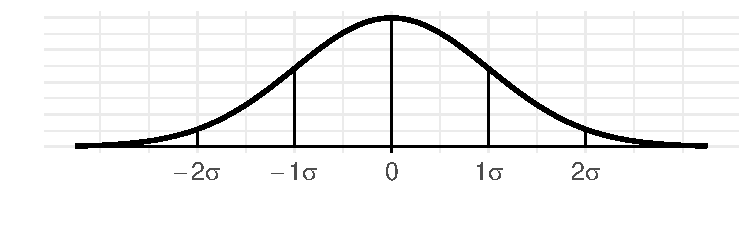
\includegraphics[width=\maxwidth]{img/mc-distribution-02-a-1} 

}







\begin{enumerate}
\item [\textbf{A} \msquare] Die Fläche rechts von $2\sigma$ ist der p-Wert mit $Pr(D|H_0)$ in der obigen Abbildung.
\item [\textbf{B} \msquare] Die Fläche zwischen $-1\sigma$ und $1\sigma$ ist 0.95 und 95\% der Beobachtungen liegen somit zwischen $\bar{y}\pm\sigma$ in der obigen Verteilung.
\item [\textbf{C} \msquare] Die Fläche zwischen $-2\sigma$ und $2\sigma$ ist 0.68 und 68\% der Beobachtungen liegen somit zwischen $\bar{y}\pm\sigma$ in der obigen Verteilung.
\item [\textbf{D} \msquare] Die Fläche unter der Kurve ist 1, wenn die Nullhypothese falsch ist. Wenn die Nullhypothese gilt, dann ist die Fläche $1-\alpha$. Somit ergibt sich auch eine Standardabweichung $\sigma$ mit $\alpha$ gleich 0.05 in beiden Fällen.
\item [\textbf{E} \msquare] Die Fläche zwischen $-2\sigma$ und $2\sigma$ ist 0.95 und 95\% der Beobachtungen liegen somit zwischen $\bar{y}\pm\sigma$ in der obigen Verteilung.
\end{enumerate} 

\section{Aufgabe \hfill (2 Punkte)}



Nachdem Sie eine ANOVA und die paarweisen t-Tests über das \Rlogo Paket \{emmeans\} durchgeführt haben, müssen Sie Ihre Daten nochmal zur Überprüfung visualisieren. Sie entscheiden sich für den Boxplot. Welche statistischen Maßzahlen stellt der Boxplot dar?

 



\begin{enumerate}
\item [\textbf{A} \msquare] Durch die Abbildung des Boxplot erhalten wir die Informationen über den Median und die Quartile.
\item [\textbf{B} \msquare] Den Median und die Standardabweichung.
\item [\textbf{C} \msquare] Der Boxplot stellt die Mittelwerte und die Varianz dar.
\item [\textbf{D} \msquare] Der Boxplot stellt den Median und die Streuung dar.
\item [\textbf{E} \msquare] Der Boxplot stellt die Mittelwerte und die Standardabweichung dar.
\end{enumerate}

\section{Aufgabe \hfill (2 Punkte)}



Der Mittelwert $\bar{y}$ und der Median $\tilde{y}$ unterscheiden sich nicht in Ihren Feldexperiment zu Leistungssteigerung von Brokoli.  Welche Aussage ist richtig?



\begin{enumerate}
\item [\textbf{A} \msquare] Der Mittelwert und der Median sollten gleich sein, wenn keine Outlier in den Daten vorliegen. 
\item [\textbf{B} \msquare] Wenn sich der Mittelwert und der Median nicht unterscheiden, liegen vermutlich keine Outlier in den Daten vor.
\item [\textbf{C} \msquare] Wenn sich der Mittelwert und der Median nicht unterscheiden, liegen vermutlich Outlier in den Daten vor.
\item [\textbf{D} \msquare] Da sich der Mittelwert und der Median unterscheiden, ist der Datensatz nicht zu verwenden. Mittelwert und Median müssen gleich sein.
\item [\textbf{E} \msquare] Wenn sich der Mittelwert und der Median unterscheiden, liegen vermutlich keine Outlier in den Daten vor.
\end{enumerate} 

\section{Aufgabe \hfill (2 Punkte)}



Mit einem Dotplot  können Sie sehr gut die Verteilung von Daten visualisieren. Die empfohlene Mindestanzahl an Beobachtungen ist dabei?



\begin{enumerate}
\item [\textbf{A} \msquare] Wir sollten zwei bis fünf Beobachtungen mindestens pro Gruppe vorliegen haben.
\item [\textbf{B} \msquare] Wir sollten eine Beobachtung mindestens pro Gruppe vorliegen haben.
\item [\textbf{C} \msquare] Wir brauchen fünf oder mehr Beobachtungen.
\item [\textbf{D} \msquare] Die untere Grenze liegt bei einer Beobachtung.
\item [\textbf{E} \msquare]  erhalten, sollten wir mindestens zwanzig Beobachtungen haben.
\end{enumerate}

\section{Aufgabe \hfill (2 Punkte)}




In der Statistik müssen wir häufig überprüfen, ob unser Outcome einer bestimmten Verteilung folgt. Meistens überprüfen wir, ob eine
Normalverteilung vorliegt. Folgende drei Abbildungen eigenen sich im Besonderen für die Überprüfung einer Verteilungsannahme an eine Variable.





\begin{enumerate}
\item [\textbf{A} \msquare] Boxplot, Violinplot, Mosaicplot
\item [\textbf{B} \msquare] Scatterplot, Densityplot, Barplot
\item [\textbf{C} \msquare] Boxplot, Densityplot, Violinplot
\item [\textbf{D} \msquare] Histogramm, Densityplot, Dotplot
\item [\textbf{E} \msquare] Scatterplot, Mosaicplot, Boxplot
\end{enumerate}

\section{Aufgabe \hfill (2 Punkte)}



Ihre Betreuung der Abschlussarbeit fragt überraschend in der letzten Besprechung, ob Ihre Messwerte einer Varianzhomogenität genügen. Sonst könnten Sie ja gar nicht einen t-Test rechnen. Da Ihnen die Zeit wegrennt, entscheiden Sie sich für eine schnelle Visualisierung im Anhang. Welche Visualisierung nutzen Sie und welche Regel kommt zur Abschätzung einer Varianzhomogenität zur Anwendung?



\begin{enumerate}
\item [\textbf{A} \msquare] Einen Dotplot. Die Punkte müssen sich wie an einer Perlenschnurr audreihen. Eine Abweichung führt zur Ablehnung der Annahme einer Varianzhomogenität.
\item [\textbf{B} \msquare] Nach dem Einlesen der Daten nutzen wir einen Boxplot um zu schauen, ob alle Boxen über alle Behandlungen in etwa gleich groß sind. Damit ist dann auch das IQR in allen Behandlungen in etwa gleich.
\item [\textbf{C} \msquare] Nach dem Einlesen der Daten nutzen wir einen Barplot um zu schauen, ob alle Mittelwerte über alle Behandlungen in etwa gleich groß sind. Damit ist dann auch die Varianz in allen Behandlungen in etwa gleich.
\item [\textbf{D} \msquare] In einer explorativen Datanalyse nutzen wir den Violinplot. Dabei sollte der Bauch am Rand liegen. Dann können wir von einer Varianzhomogenität ausgehen.
\item [\textbf{E} \msquare] In einer explorativen Datanalyse nutzen wir den Boxplot. Dabei sollte der Median als dicke Linie in der Mitte der Box liegen. Dann können wir von einer Varianzhomogenität ausgehen.
\end{enumerate}
\section*{Statistische Testtheorie}  

\section{Aufgabe \hfill (2 Punkte)}




Geben ist $Pr(D|H_0)$ als mathematischer Ausdruck, welche Aussage ist richtig?



\begin{enumerate}
\item [\textbf{A} \msquare] $Pr(D|H_0)$ ist die Wahrscheinlichkeit nicht die Daten $D$ zu beobachten sondern die Nullhypothese, wenn diese wahr ist.
\item [\textbf{B} \msquare] $Pr(D|H_0)$ stellt die Wahrscheinlichkeit die Daten $D$ und somit die Teststatistik $T_D$ zu beobachten dar, wenn die Nullhypothese wahr ist.
\item [\textbf{C} \msquare] $Pr(D|H_0)$ stellt die Wahrscheinlichkeit die Teststatistik $T$ zu beobachten dar, wenn die Nullhypothese falsch ist.
\item [\textbf{D} \msquare] Die Wahrscheinlichkeit für die Nullhypothese, wenn die Daten wahr sind.
\item [\textbf{E} \msquare] Die Wahrscheinlichkeit der Daten unter der Nullhypothese in der Grundgesamtheit.
\end{enumerate} 

\section{Aufgabe \hfill (2 Punkte)}



Das statistische Testen basiert auf dem Falsifikationsprinzip. Es besagt,



\begin{enumerate}
\item [\textbf{A} \msquare] ... dass in der Wissenschaft immer etwas falsch sein muss. Sonst gebe es keinen Fortschritt.
\item [\textbf{B} \msquare] ... dass ein schlechtes Modell durch das Falsifikationsprinzip durch ein noch schlechteres Modell ersetzt wird. Die Wissenschaft lehnt ab und verifiziert nicht.
\item [\textbf{C} \msquare] ... dass ein schlechtes Modell durch ein schlechteres Modell ersetzt wird. Die Wissenschaft lehnt ab und verifiziert nicht.
\item [\textbf{D} \msquare] ... dass Fehlerterme in statistischen Modellen nicht verifiziert werden können.
\item [\textbf{E} \msquare] ... dass ein schlechtes Modell durch ein weniger schlechtes Modell ersetzt wird. Die Wissenschaft lehnt ab und verifiziert nicht.
\end{enumerate} 

\section{Aufgabe \hfill (2 Punkte)}



Der Fehler 1. Art oder auch Signifikanzniveau $\alpha$ genannt, liegt bei
5\%. Welcher der folgenden Gründe für diese Festlegeung auf 5\% als Signifikanzschwelle ist richtig?



\begin{enumerate}
\item [\textbf{A} \msquare] In der Wissenschaft gibt es neben der Naturkonstante, die sich aus der Beobachtung der Welt ergibt, noch die Kulturkonstante, die von einer Gruppe Menschen selbstgewählt wird. Dabei ist $\alpha = 5\%$ eine Kulturkonstante und wurde somit eher zufällig gewählt.
\item [\textbf{B} \msquare] Als Kulturkonstante hat $\alpha = 5\%$ den Rang einer Naturkonstante und wurde nach langer Diskussion in der UN im Jahre 1983 festgesetzt. Damals auch schon mit der Zustimmung der UdSSR.
\item [\textbf{C} \msquare] Da Wissenschaftler eine Schwelle für die statistische Testentscheidung benötigen wurde $\alpha$ in einer großen Konferenz 1945 gewählt. Damit ist $\alpha = 5\%$ eine Kulturkonstante mit einem Rank einer Naturkonstante.
\item [\textbf{D} \msquare] Auf einer Statistikkonferenz in Genf im Jahre 1942 wurde dieser Cut-Off nach langen Diskussionen festgelegt. Bis heute ist der Cut Off aber umstritten, da wegen dem 2. Weltkrieg viele Wissenschaftler nicht teilnehmen konnten.
\item [\textbf{E} \msquare] Der Wert ergab sich aus einer Auswertung von 1042 wissenschaftlichen Veröffentlichungen zwischen 1914 und 1948. Der Wert $5\%$ wurde in $28\%$ der Veröffentlichungen genutzt. Daher legte man sich auf diese Zahl fest.
\end{enumerate}

\section{Aufgabe \hfill (2 Punkte)}

Betrachten wir die Teststatistik aus einem abstrakteren Blickwinkel. Beim
statistischen Testen wird das \textit{"`signal"'} mit dem
\textit{"`noise"'} aus den Daten $D$ zu einer Teststatistik $T_D$ verrechnet. Welche der Formel
berechnet korrekt die Teststatistik $T_D$?



\begin{enumerate}
\item [\textbf{A} \msquare] Es gilt $T_D = \cfrac{signal}{noise^2}$
\item [\textbf{B} \msquare] Es gilt $T_D = signal \cdot noise$
\item [\textbf{C} \msquare] Es gilt $T_D = \cfrac{noise}{signal}$
\item [\textbf{D} \msquare] Es gilt $T_D = \cfrac{signal}{noise}$
\item [\textbf{E} \msquare] Es gilt $T_D = (signal \cdot noise)^2$
\end{enumerate}

%% ------------------------------------------------------------

\section{Aufgabe \hfill (2 Punkte)}



Sie haben ein Signifikanzniveau $\alpha$ gleich 5\% vorliegen. Welche Aussage zusammen mit dem $p$-Wert ist richtig?



\begin{enumerate}
\item [\textbf{A} \msquare] Wir vergleichen mit dem $p$-Wert und dem Signifikanzniveau $\alpha$ absolute Werte auf einem Zahlenstrahl und damit den Unterschied der Teststatistiken, wenn die $H_0$ gilt.
\item [\textbf{B} \msquare] Wir machen ein Aussage über die Flächen und zwischen den Kurve der Teststatistiken der Hypothesen $H_0$ und $H_A$, wenn die $H_0$ gilt. Dabei werden Wahrscheinlichkeiten vergleichen, die durch die Flächen unter der Kurve repräsentiert werden.
\item [\textbf{C} \msquare] Wir vergleichen die Effekte des $p$-Wertes mit den Effekten der Signifikanzschwelle unter der Annahme der Nullhypothese. Dabei gilt, dass wir die Nullhypothese nur ablehnen können anhand des Falsifikationsprinzips.
\item [\textbf{D} \msquare] Wir schauen, ob der $p$-Wert kleiner ist als das Signifikanzniveau $\alpha$ und vergleichen somit Wahrscheinlichkeiten. Die Wahrscheinlichkeiten werden als Flächen unter der Kurve der Teststaistik dargestellt, wenn die $H_0$ gilt.
\item [\textbf{E} \msquare] Wir vergleichen mit dem $p$-Wert und dem Signifikanzniveau $\alpha$ Wahrscheinlichkeiten und damit die absoluten Werte auf einem Zahlenstrahl, wenn die $H_0$ gilt.
\end{enumerate}

\section{Aufgabe \hfill (2 Punkte)}



Die Ergebnisse der einer statistischen Analyse können in die Analogie einer Wettervorhersage gebracht werden. Welche Analogie für die Ergebnisse eines statistischen Tests trifft am besten zu?



\begin{enumerate}
\item [\textbf{A} \msquare] In der Analogie der Maximaltemperatur: Was ist der maximale Unterschied zwischen zwei Gruppen. Wir erhalten hier eine Aussage über die Spannweite und den maximalen Effekt.
\item [\textbf{B} \msquare] In der Analogie des Niederschlags oder Regenmenge: ein statistischer Test gibt die Stärke eines Effektes wieder. Zum Beispiel, wie hoch ist der Mittelwertsunterschied.
\item [\textbf{C} \msquare] In der Analogie der Sonnenscheindauer: Wie lange kann mit einem entsprechenden Effekt gerechnet werden? Die Wahrscheinlichkeit für den Effekt gibt der statistische Test wieder.
\item [\textbf{D} \msquare] In der Analogie der Durchschnittstemperatur: Wie oft tritt ein Effekt durchschnittlich ein? Wir erhalten eine Wahrscheinlichkeit für die Effekte. Zum Beispiel, wie hoch ist die Wahrscheinlichkeit für einen Mittelwert als Durchschnitt.
\item [\textbf{E} \msquare] In der Analogie der Wahrscheinlichkeit für Regen: ein statistischer Test erlaubt die Wahrscheinlichkeit für ein Ereignis abzuschätzen. Die Stärke des Effektes können wir nicht bestimmen.
\end{enumerate}

\section{Aufgabe \hfill (2 Punkte)}



In Ihrer Forschungsarbeit wollen Sie eine Aussage über ein untersuchtes Individuum treffen. Dazu nutzen Sie einen statistischen Test. Erhalten Sie eine valide Aussage aus einem statistischen Test?



\begin{enumerate}
\item [\textbf{A} \msquare] Ja, ein untersuchtes Individuum können wir mit einem statistischen Test auswerten. Wir erhalten dann eine Aussage zum Individuum.
\item [\textbf{B} \msquare] Nein, wir erhalten eine Aussage. Müssen aber das Individuum im Kontext der Population adjustieren.
\item [\textbf{C} \msquare] Nein, wir erhalten nur eine Aussage zu zwei Individuen. Ein statistischer Test liefert Informationen zu einem Individuum im Vergleich zu einem anderen Individuum.
\item [\textbf{D} \msquare] Nein, wir können ein untersuchtes Individuum nicht mit einer ANOVA auswerten. Wir erhalten keine Aussage zum Individuum.
\item [\textbf{E} \msquare] Ja, wir können ein untersuchtes Individuum nicht mit einem t-Test auswerten. Wir erhalten keine Aussage zum Individuum. Wir können aber den Effekt als Quelle der Relevanz nutzen.
\end{enumerate}

\section{Aufgabe \hfill (2 Punkte)}



In Ihrer Abschlussarbeit sollen Sie neben den p-Werten auch die Effekte mit angeben. Welche Aussage ist richtig?



\begin{enumerate}
\item [\textbf{A} \msquare] Der Effekt eines statistischen Tests beschreibt die biologisch interpretierbare Ausgabe eines Tests. Moderen Algorithmen liefern keine Effekte mehr sondern nur noch bedingte Wahrscheinlichkeiten. Der Effekt spielt in der modernen Statistik keine Rollen mehr.
\item [\textbf{B} \msquare] Durch den Effekt erfahren wir die statistische interpretierbare Ausgabe eines statistischen Tests. Zum Beispiel das $\eta^2$ aus einer ANOVA. Damit können wir die Signifikanz direkt mit dem Effekt verbinden. Am Ende muss der Forschende aber entscheiden, ob der Effekt entsprechend seinen Erwartungen als bedeutet zu bewerten ist.
\item [\textbf{C} \msquare] Der Effekt eines statistischen Tests beschreibt die biologisch interpretierbare Ausgabe eines Tests. Damit ist der Effekt direkt mit dem Begriff der Signifikanz verbunden. Die Entscheidung über die Signifikanz trifft der Forschende unabhängig von der Relevanz eines statistsichen Tests.
\item [\textbf{D} \msquare] Der Effekt eines statistischen Tests beschreibt den Output oder die Wiedergabe eines Tests in einem Computer.
\item [\textbf{E} \msquare] Der Effekt eines statistischen Tests beschreibt die biologisch interpretierbare Ausgabe eines Tests. Zum Beispiel den mittleren Unterschied zwischen zwei Gruppen aus einem t-Test. Damit ist der Effekt direkt mit dem Begriff der Relevanz verbunden. Die Entscheidung über die Relevanz trifft der Forschende unabhängig von der Signifikanz eines statistischen Tests.
\end{enumerate}

\section{Aufgabe \hfill (2 Punkte)}

Die Randomisierung von Beobachtungen zu den Versuchseinheiten
ist bedeutend in der Versuchsplanung. Welche der folgenden Aussagen ist richtig?



\begin{enumerate}
\item [\textbf{A} \msquare] Randomisierung erlaubt erst die Mittelwerte zu schätzen. Ohne Randomisierung keine Mittelwerte. Ohne Mittelwerte keine Varianz und somit auch kein statistischer Test.
\item [\textbf{B} \msquare] Randomisierung war bis 1952 bedeutend, wurde dann aber in Folge besserer Rechnerleistung nicht mehr verwendet. Aktuelle Statistik nutzt keine Randomisierung mehr.
\item [\textbf{C} \msquare] Durch eine Randomisierung können wir nicht von Strukturgleichheit zwischen der Stichprobe und der Grundgesamtheit ausgehen.
\item [\textbf{D} \msquare] Randomisierung sorgt für Strukturgleichheit und erlaubt erst von der Stichprobe auf die Grundgesamtheit zurückzuschliessen.
\item [\textbf{E} \msquare] Strukturgleichheit ist durch Randomisierung gegeben. Leider hilft die Randomisierung noch nicht um von der Stichprobe auf die Grundgesamtheit zu schließen. Deshalb wurde das Falsifikationsprinzip entwickelt.
\end{enumerate}

\section{Aufgabe \hfill (2 Punkte)}



Ein statistischer Test benötigt für die richtige Durchführung Hypothesen $H$, sonst ist der Test nicht zu interpretieren. Welche Aussage ist richtig?



\begin{enumerate}
\item [\textbf{A} \msquare] Ein statistisches Hypothesenpaare gibt es. Zum einen die Nullhypothese und zum anderen die Alternativehypothese. Es ist aber nur notwendig die Alternative anzugeben, da die Nullhypothese nicht beim Testen benötigt wird.
\item [\textbf{B} \msquare] Es gibt ein Hypothesenset bestehend aus $k$ Hypothesen. Meistens wird die Nullhypothese $H_0$ und die Alternativhypothese $H_A$ verwendet. Wegen des Falsifikationsprinzips ist es wichtig, die bekannte falsche und unbekannte richtige Hypothese mit in das Set zu nehmen.
\item [\textbf{C} \msquare] Es gibt ein statistisches Hypothesenpaar mit der Hypothese für und gegen die wissenschaftliche Fragestellung. Die Hypothesen werden $H_{pro}$ und $H_{contra}$ bezeichnet.
\item [\textbf{D} \msquare] Mit der Nullhypothese $H_0$ und der Alternativehypothese $H_A$ oder $H_1$ gibt es zwei Hypothesen.
\item [\textbf{E} \msquare] Die Hypothesen $H_0$ und $H_A$ sind rein prosarischer Natur und bilden keinen mathematischen Hintergrund ab. In der Statistik wird die wissenschaftliche Fragestellung getestet. Daher stehen auch die verständlichen Hypothesen im Mittelpunkt der biologischen Interpretation.
\end{enumerate}

\section{Aufgabe \hfill (2 Punkte)}



Sie versuchen folgende Aussage richtig in die Analogie der statistischen Testtheorie zu setzen. Welche Analogie ist richtig?

\begin{center}
\textit{$H_0$ ablehnen obwohl die $H_0$ gilt}
\end{center}



\begin{enumerate}
\item [\textbf{A} \msquare] \textit{Fire without alarm}, dem $\beta$-Fehler als Analogie von Rauch im Haus.
\item [\textbf{B} \msquare] In die Analogie eines Feuerwehrautos: \textit{Car without noise}.
\item [\textbf{C} \msquare] In die Analogie eines Rauchmelders: \textit{Alarm without fire police}, dem $\alpha$-Fehler.
\item [\textbf{D} \msquare] \textit{Alarm without fire}, dem $\alpha$-Fehler in der Analogie eines Rauchmelders.
\item [\textbf{E} \msquare] Dem $\beta$-Fehler mit der Analogie eines Rauchmelders: \textit{Fire without alarm}.
\end{enumerate}

\section{Aufgabe \hfill (2 Punkte)}



Welche statistische Maßzahl erlaubt es Relevanz mit Signifikanz zu verbinden? Welche Aussage ist richtig?



\begin{enumerate}
\item [\textbf{A} \msquare] Das OR. Als Chancenverhältnis gibt es das Verhältnis von Relevanz und Signifikanz wieder.
\item [\textbf{B} \msquare] Die Teststatistik. Durch den Vergleich von $T_c$ zu $T_k$ ist es m{"o}glich die $H_0$ abzulehnen. Die Relevanz ergibt sich aus der Fläche rechts vom dem $T_c$-Wert.
\item [\textbf{C} \msquare] Über das Konfidenzintervall. Das Konfidenzinterval inkludiert eine Entscheidung über die Relevanz und zusätzlich kann über die Visualizierung des Konfidenzintervals eine Signifikanzschwelle vom Forschenden definiert werden.
\item [\textbf{D} \msquare] Über das Konfidenzintervall. Das Konfidenzinterval beitet eine Entscheidung über die Signifikanz und zusätzlich kann über die Visualizierung des Konfidenzintervals eine Relevanzschwelle definiert werden.
\item [\textbf{E} \msquare] Der p-Wert. Durch den Vergleich mit $\alpha$ lässt sich über die Signifikanz entscheiden und der $\beta$-Fehler erlaubt über die Power eine Einschätzung der Relevanz.
\end{enumerate}

\section{Aufgabe \hfill (2 Punkte)}



Historisch gesehen ergibt sich ein Problem, wenn Sie mit sehr großen Datensätzen, wie in der Bio Data Sience üblich, rechnen. Warum ist es ein Problem, wenn Ihre Datensätze sehr groß werden hinsichtlich der Bewertung anhand der Signifikanz?




\begin{enumerate}
\item [\textbf{A} \msquare] Eine erhöhte Fallzahl führt automatisch zu mehr signifikanten Ergebnissen auch wenn der Effekt klein ist und damit nicht relevant. Dadurch sind die Informationen zur Signifikanz in riesigen Datensätzen schwer zu verwerten, da fast alle Vergleiche signifikant sind.
\item [\textbf{B} \msquare] Aktuell werden immer größere Datensätze erhoben. Dadurch wird auch die Varianz immer höher was automatisch zu mehr signifikanten Ergebnissen führt.
\item [\textbf{C} \msquare] Riesige Datensätz haben mehr Fallzahl was zur $\alpha$-Inflation führt. Durch eine Adjustoerung kann dem Problem entgegengewirkt werden.
\item [\textbf{D} \msquare] Aktuell werden zu grosse Datensätze für die gänigige Statistik gemessen. Daher wendet man maschinelle Lernverfahren für kausale Modelle an. Hier ist die Relevanz gleich Signifikanz.
\item [\textbf{E} \msquare] Relevanz und Signifikanz haben nichts miteinander zu tun. Daher gibt es auch keinen Zusammenhang zwischen hoher Fahlzahl (n > 10000) und einem signifikanten Test. Ein Effekt ist immer relevant und somit signifikant.
\end{enumerate}

\section{Aufgabe \hfill (2 Punkte)}



In einem Zuchtexperiment messen wir die Ferkel verschiedener Sauen. Die Ferkel einer Muttersau sind daher im statistischen Sinne...



\begin{enumerate}
\item [\textbf{A} \msquare] Die Ferkel stammen vom gleichen Muttertier und haben vermutlich eine ähnlichere Varianzstruktur als die Ferkel von anderen Sauen. Die Ferkel sind untereinander über die Mutter abhängig.
\item [\textbf{B} \msquare] Untereinander stark korreliert. Die Ferkel sind von einer Mutter und sommit miteinander korreliert. Dies wird in der Statistik jedoch meist nicht modelliert.
\item [\textbf{C} \msquare] Abhängig von der Stallanlage und des Experiments können die Ferkel abhängig oder unabhängig sein. Allgmein gilt, dass Ferkel von unterschiedlichen Sauen näher miteinander verwandt sind als Ferkel von gleichen Sauen. Das Fisher-Axiom.
\item [\textbf{D} \msquare] Untereinander unabhängig. Sollten die Mütter verwandt sein, so ist die Varianzstruktur ähnlich und muss modelliert werden.
\item [\textbf{E} \msquare] Die Ferkel stammen von der gleichen Sau und sind somit untereinander unabhängig.
\end{enumerate}

\section{Aufgabe \hfill (2 Punkte)}





Sie rechnen einen statistischen Test und wollen anhand des 95\%-Konfidenzintervalls eine Entscheidung gegen die Nullhypothese treffen. Welche Aussage ist richtig?





\begin{enumerate}
\item [\textbf{A} \msquare] Anhand des 95\%-Konfidenzintervalls lässt sich wie folgt eine Entscheidung treffen. Ist die Null mit enthalten, dann kann die Nullhypothese abgelehnt werden.
\item [\textbf{B} \msquare] Das Signifikanzniveauintervall $\alpha$ ist gleich $5\%$ und damit muss das berechnete Intervall unter dem Signifikanzniveauintervall $\alpha$ liegen, dann kann die Nullhypothese nicht abgelehnt werden.
\item [\textbf{C} \msquare] Ist $Pr(D|H_0)$ kleiner als das Signifikanzniveau $\alpha$ gleich $5\%$ dann wird die Nullhypothese $H_0$ abgelehnt.
\item [\textbf{D} \msquare] Der kritische Wert $T_{\alpha = 5\%}$ ist tabelarisch festgelegt und gegeben. Ist $T_{D}$ größer als der kritische Wert, kann die Nullhypothese abgelehnt werden
\item [\textbf{E} \msquare] Das Signifikanzniveau $\alpha$ ist gleich $5\%$ und das berechnete Intervall muss gleich\textit{er} als das Signifikanzniveau sein.
\end{enumerate}

\section{Aufgabe \hfill (2 Punkte)}



Welche Aussage über die \textit{Power} ist richtig?



\begin{enumerate}
\item [\textbf{A} \msquare] Die Power ist nicht in der aktuellen Testthorie mehr vertreten. Wir rechnen nur noch mit dem Fehler 1. Art.
\item [\textbf{B} \msquare] Alle statistischen Tests sind so konstruiert, dass die $H_A$ mit 20\% \textit{bewiesen wird}. Die Power ist $1-\beta$ mit $\beta$ gleich 80\% gesetzt.
\item [\textbf{C} \msquare] Es gilt $\alpha + \beta = 1$ und somit liegt $\beta$ meist bei 95\%.
\item [\textbf{D} \msquare] Die Power wird nicht berechnet sondern ist eine Eigenschaft des Tests. Die Power wird auf $80\%$ gesetzt und beschreibt mit welcher Wahrscheinlichkeit $H_A$ \textit{bewiesen wird}
\item [\textbf{E} \msquare] Die Power $1-\beta$ wird auf 80\% gesetzt. Damit liegt die Wahrscheinlichkeit für die $H_0$ bei 20\%.
\end{enumerate}
\section*{Statistische Tests für Gruppenvergleiche} 

\section{Aufgabe \hfill (2 Punkte)}



Nach einem Feldexperiment wollen Sie zwei Gruppen mit einem Welch t-Test vergleichen. Welche Aussage ist auch für den Student t-Test richtig?



\begin{enumerate}
\item [\textbf{A} \msquare] Der t-Test vergleicht zwei Gruppen indem die Mittelwerte miteinander verglichen werden.
\item [\textbf{B} \msquare] Der t-Test vergleicht zwei oder mehr Gruppen indem die Mittelwerte miteinander verglichen werden.
\item [\textbf{C} \msquare] Der t-Test vergleicht die Mittelwerte von zwei Gruppen unter der strikten Annahme von Varianzhomogenität. Sollte keine Varianzhomogenität vorliegen, so gibt es keine Möglichkeit den t-Test in einer Variante anzuwenden.
\item [\textbf{D} \msquare] Der t-Test testet generell zu einem erhöhten $\alpha$-Niveau von 20\%.
\item [\textbf{E} \msquare] Der t-Test vergleicht die Varianzen von mindestens zwei oder mehr Gruppen
\end{enumerate}

\section{Aufgabe \hfill (2 Punkte)}



Ein Versuch wurde in 8 Parzellen pro Gruppe durchgeführt. Die folgende Abbildung enthält die Daten aus diesem Versuch zur Bewertung der Wirkung des Mikronährstoff Eisen auf den Ertrag in t/ha von Weizen im Vergleich zu einer Kontrolle.  Welche Aussage ist richtig, wenn Sie einen t-Test rechnen?



{\centering 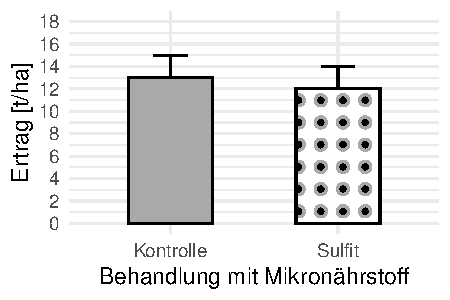
\includegraphics[width=\maxwidth]{img/mc-testing-ttest-02-1} 

}







\begin{enumerate}
\item [\textbf{A} \msquare] Die Barplots deuten auf keinen signifikanten Unterschied. Der Effekt liegt vermutlich bei -7 unter einer groben Abschätzung.
\item [\textbf{B} \msquare] Es liegt ein signifikanter Unterschied vor. Der Effekt liegt bei -0.7.
\item [\textbf{C} \msquare] Die Barplots deuten auf keinen signifikanten Unterschied. Der Effekt liegt vermutlich bei -7 unter einer groben Abschätzung. Wir müssen aber eine ANOVA rechnen um den Effekt wirklich bestimmen zu können.
\item [\textbf{D} \msquare] Der Effekt und die Signifikanz lassen sich nicht aus Barplots abschätzen. Höchtens der Effekt als relativer Unterschied zwischen der Höhe der Barplots. Standard ist der mediane Unterschied aus Boxplots.
\item [\textbf{E} \msquare] Der Test deutet auf ein signifikanten Unterschied hin. Der Effekt liegt vermutlich bei -7.
\end{enumerate}

\section{Aufgabe \hfill (2 Punkte)}




In Ihrer Abschlussarbeit betrachten Sie die Effekte von einer Behandlung vor und nach der Gabe eines Vitamins. Sie müssen einen gepaarten t-Test rechnen. Welche Aussage ist richtig?



\begin{enumerate}
\item [\textbf{A} \msquare] Wenn die Beobachtungen unabhängig voneinander sind, rechnen wir einen gepaarten t-Test. Messen wir wiederholt an dem gleichen Tier oder Pflanze dann bilden wir das Produkt zwischen den zwei Messpunkten.
\item [\textbf{B} \msquare] Beim gepaarten t-Test kombinieren wir die Vorteile des Student t-Test für Varianzhomogenität mit den Vorteilen des Welch t-Test für Varianzheterogenität. Wir bilden dafür die Differenz der Einzelbeobachtungen.
\item [\textbf{C} \msquare] Abhängige Beobachtungen müssen gesondert in einem gepaarten t-Test modelliert werden. Wenn wiederholt an dem gleichen Tier oder Pflanze gemessen wird, dann bilden wir den Quotienten zwischen den beiden Zeitpunkten. Auf den Quotienten rechnen wir den gepaarten t-Test.
\item [\textbf{D} \msquare] Der gepaarte t-Test nutzt die Varianz der Beobachtungen jeweils paarweise und bildet dafür eine verbundene Stichprobe. Dieser Datensatz $d$ dient dann zur Differenzbildung.
\item [\textbf{E} \msquare] Abhängige Beobachtungen müssen gesondert in einem gepaarten t-Test modelliert werden. Wenn wiederholt an dem gleichen Tier oder Pflanze gemessen wird, dann bilden wir die Differenz zwischen den beiden Zeitpunkten. Auf den Differenzen rechnen wir den gepaarten t-Test.
\end{enumerate}

\section{Aufgabe \hfill (2 Punkte)}



Nach einem Experiment mit drei Weizensorten ergibt eine ANOVA ($p = 0.049$) einen signifikanten Unterschied für den Ertrag. Sie führen anschließend die paarweisen t-Tests für alle Vergleiche der verschiedenen Weizensorten durch. Nach der Adjustierung für multiples Testen ist kein p-Wert unter der $\alpha$-Schwelle. Sie schauen sich auch die rohen, unadjustierten p-Werte an und finden hier als niedrigsten p-Wert $p_{3-2} = 0.053$. Welche Aussage ist richtig?




\begin{enumerate}
\item [\textbf{A} \msquare] Die adjustierten p-Werte deuten in die richtige Richtung. Zusammen mit den nicht signifikanten rohen p-Werten ist von einem Fehler in der ANOVA auszugehen.
\item [\textbf{B} \msquare] Es gibt einen Fehler in der Varianzstruktur. Daher kann die ANOVA nicht richtig sein und paarweise t-Tests liefern das richtige Ergebnis.
\item [\textbf{C} \msquare] Hier kommt der Effekt der stiegenden Fallzahl auf die Anzahl an signifikante Ergebnisse zu tragen. Da die ANOVA auf weniger Fallzahl testet als die paarweisen t-Tests, kann die ANOVA schwerer einen signifikanten Unterscheid nachweisen.
\item [\textbf{D} \msquare] Das ist kein Wunder. Die ANOVA testet nicht auf der gesamten Fallzahl und die paarweisen t-Tests gewinnen immer eine oder mehr Gruppen als Fallzahl dazu. Mit steigender Fallzahl sind mehr signifikante Unterschiede zu erwarten. Die p-Werte unterscheiden sich numerisch auch kaum.
\item [\textbf{E} \msquare] Das ist kein Wunder. Die ANOVA testet auf der gesamten Fallzahl und die paarweisen t-Tests verlieren immer eine oder mehr Gruppen als Fallzahl. Mit steigender Fallzahl sind mehr signifikante Unterschiede zu erwarten. Die p-Werte unterscheiden sich numerisch auch kaum.
\end{enumerate}
\section*{ANOVA}

\section{Aufgabe \hfill (2 Punkte)}





Sie führen einen Versuch mit einer Behandlung und drei Faktorleveln durch. Danach rechnen Sie eine einfaktorielle ANOVA und es ergibt sich ein $\eta^2 = 0.52$. Welche Aussage ist richtig?



\begin{enumerate}
\item [\textbf{A} \msquare] Das $\eta^2$ ist ein Wert f{"u}r die G{"u}te der ANOVA. Je kleiner desto besser. Ein $\eta^2$ von 0 bedeutet ein perfektes Modell mit keiner Abweichung. Die Varianz ist null.
\item [\textbf{B} \msquare] Das $\eta^2$ ist die Korrelation der ANOVA. Mit der Ausnahme, dass 0 der beste Wert ist.
\item [\textbf{C} \msquare] Das $\eta^2$ beschreibt den Anteil der Varianz, der von den Behandlungsbedingungen erkl{"a}rt wird. Das $\eta^2$ ist damit mit dem $R^2$ aus der linearen Regression zu vergleichen.
\item [\textbf{D} \msquare] Die Berechnung von $\eta^2$ ist ein Wert f{"u}r die Interaktion.
\item [\textbf{E} \msquare] Das $\eta^2$ beschreibt den Anteil der Varianz, der von den Behandlungsbedingungen nicht erkl{"a}rt wird. Somit der Rest an nicht erkl{"a}rbarer Varianz.
\end{enumerate}

\section{Aufgabe \hfill (2 Punkte)}



Sie führen ein Feldexperiment durch um das Gewicht von Kartoffel zu
steigern. Die Pflanzen wachsen unter einer Kontrolle und zwei verschiedenen
Behandlungsbedingungen. Nach der Berechnung einer einfaktoriellen ANOVA
ergibt sich ein $\eta^2 = 0.24$. Welche Aussage ist richtig?



\begin{enumerate}
\item [\textbf{A} \msquare] Mit dem $\eta^2$ lässt sich auf die Qualität der Randomisierung und damit der Strukturgleichheit zwischen der Grundgesamtheit und der Stichprobe schließen. Es gilt dabei die Regel, dass ein $\eta^2$-Wert von 1 zu bevorzugen ist.
\item [\textbf{B} \msquare] Das $\eta^2$ beschreibt den Anteil der Varianz, der durch den Forschenden entsteht. Es gilt die Regel, dass ca. 70\% der Varianz eines Versuches durch die Versuchsdurchführung entstehen sollen.
\item [\textbf{C} \msquare] Das $\eta^2$ beschreibt den Anteil der Varianz, der von den Behandlungsbedingungen erklärt wird. Daher werden 24\% der Varianz erklärt.
\item [\textbf{D} \msquare] Es werden 76\% der Varianz durch die Behandlung erklärt. Das $\eta^2$ beschreibt den Anteil der Varianz, der von den unterschiedlichen Behandlungsbedingungen nicht erklärt wird.
\item [\textbf{E} \msquare] Es werden 24\% der Varianz durch den Versuch erklärt. Das $\eta^2$ beschreibt den Anteil der Varianz, der durch Fehler in der Versuchsdurchführung entsteht.
\end{enumerate}

\section{Aufgabe \hfill (2 Punkte)}



Eine einfaktorielle ANOVA berechnet eine Teststatistik um zu die Nullhypothese abzulehnen. Welche Aussage über die Teststatistik der ANOVA ist richtig?



\begin{enumerate}
\item [\textbf{A} \msquare] Die ANOVA berechnet die T-Statistik aus der Multiplikation der MS Behandlung mit der MS der Fehler. Wenn die F-Statistik genau 0 ist, kann die Nullhypothese nicht abgelehnt werden.
\item [\textbf{B} \msquare] Die ANOVA berechnt die F-Statistik aus den SS Behandlung geteilt durch die SS Fehler.
\item [\textbf{C} \msquare] Die F-Statistik wird berechnet indem die MS der Behandlung durch die MS des Fehlers geteilt werden. Wenn die F-Statistik sich kaum von der Null unterscheidet kann die Nullhypothese nicht abgelehnt werden.
\item [\textbf{D} \msquare] Wenn die F-Statistik höher ist als der kritische Wert kann die Nullhypothese nicht abgelehnt werden. Die F-Statistik ist die Differenz der MS der Behandlung durch die MS des Fehlers.
\item [\textbf{E} \msquare] Die ANOVA berechnet die F-Statistik indem die MS des Fehlers durch die MS der Behandlung geteilt werden. Wenn die F-Statistik sich der 0 ann{"a}hert kann die Nullhypothese abgelehnt werden.
\end{enumerate}

\section{Aufgabe \hfill (2 Punkte)}




Wenn Sie mehr als zwei Gruppen als Behandlungen vorliegen haben, dann kann ein einfacher t-Test nicht für den globalen Vergleich genutzt werden. Sie entscheiden sich für eine ANOVA in \Rlogo. Die ANOVA analysiert dabei...



\begin{enumerate}
\item [\textbf{A} \msquare] ... den Unterschied zwischen der globalen Varianz und der Varianz aus verschiedenen Behandlungsguppen. Wenn die ANOVA signifikant ist, ist nicht bekannt welcher Vergleich konkret unterschiedlich ist.
\item [\textbf{B} \msquare] ... den Unterschied zwischen der Mittelwerte und der Varianz aus verschiedenen Behandlungsguppen. Wenn die ANOVA signifikant ist, ist bekannt welcher Vergleich konkret unterschiedlich ist.
\item [\textbf{C} \msquare] ... den Unterschied zwischen der Varianz durch verschiedene Behandlungsguppen unter der Varianz über alle Behandlungsgruppen. Wenn die ANOVA signifikant ist, kann kein Effekt $\eta^2$ bestimmt werden.
\item [\textbf{D} \msquare] ... den Unterschied zwischen der F-Statistik anhand der Varianz der Gruppen. Wenn die F-Statistik exakt 0 ist, kann die Nullhypothese abgelehnt werden.
\item [\textbf{E} \msquare] ... den Unterschied zwischen der Varianz ausgelöst durch alle Behandlungsgruppen und der Varianz aus globalen Behandlungsguppen der Kontrollen. Wenn die ANOVA nicht signifikant ist, muss ein Posthoc-Test ausgeschlossen werden.
\end{enumerate}

\section{Aufgabe \hfill (2 Punkte)}



In einer Studie zur Bewertung der Wirkung von Vitamin E auf das Zahnwachstum bei Hasen entstand folgende Abbildung. Der Versuch wurde an 60 Tieren durchgeführt, wobei jedes Tier eine von  drei Vitamin-C-Dosen (0.5, 1 und 1.5 mg/Tag) über eine von zwei Verabreichungsmethoden erhielt. Welche Aussage ist im Bezug auf eine zweifaktorielle ANOVA richtig?



{\centering 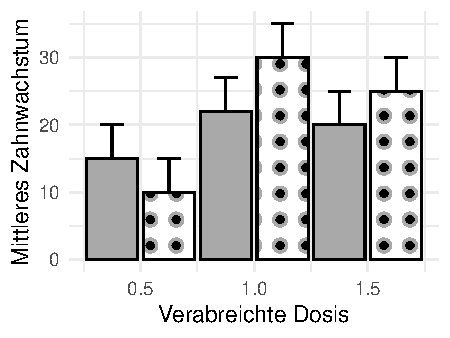
\includegraphics[width=\maxwidth]{img/mc-anova-02-a-1} 

}







\begin{enumerate}
\item [\textbf{A} \msquare] Das Bestimmtheitsmaß $R^2$ ist groß.
\item [\textbf{B} \msquare] Eine negative Interaktion liegt vor $(\rho \geq 0.5)$.
\item [\textbf{C} \msquare] Eine mittlere bis starke Interaktion liegt vor $(p \leq 0.05)$
\item [\textbf{D} \msquare] Keine Interaktion liegt vor $(p \leq 0.05)$.
\item [\textbf{E} \msquare] Die Koeffizienten sind negativ $(\beta_0 < 0; \beta_1 < 0)$.
\end{enumerate}
\section*{Multiple Gruppenvergleiche} 

\section{Aufgabe \hfill (2 Punkte)}



Sie haben folgende unadjustierten p-Werte gegeben: 0.34, 0.03, 0.01 und 0.02. Sie adjustieren die p-Werte nach
Bonferroni. Welche Aussage ist richtig?



\begin{enumerate}
\item [\textbf{A} \msquare] Nach der Bonferroni-Adjustierung ergeben sich die adjustierten p-Werte von 1, 0.12, 0.04 und 0.08. Die adjustierten p-Werte werden zu einem $\alpha$-Niveau von 5\% verglichen.
\item [\textbf{B} \msquare] Nach der Bonferroni-Adjustierung ergeben sich die adjustierten p-Werte von 1, 0.12, 0.04 und 0.08. Die adjustierten p-Werte werden zu einem $\alpha$-Niveau von 1.25\% verglichen.
\item [\textbf{C} \msquare] Nach der Bonferroni-Adjustierung ergeben sich die adjustierten p-Werte von 0.085, 0.0075, 0.0025 und 0.005. Die adjustierten p-Werte werden zu einem $\alpha$-Niveau von 1.25\% verglichen.
\item [\textbf{D} \msquare] Nach der Bonferroni-Adjustierung ergeben sich die adjustierten p-Werte von 0.085, 0.0075, 0.0025 und 0.005. Die adjustierten p-Werte werden zu einem $\alpha$-Niveau von 5\% verglichen.
\item [\textbf{E} \msquare] Nach der Bonferroni-Adjustierung ergeben sich die adjustierten p-Werte von 1.36, 0.12, 0.04 und 0.08. Die adjustierten p-Werte werden zu einem $\alpha$-Niveau von 5\% verglichen.
\end{enumerate}

\section{Aufgabe \hfill (2 Punkte)}



Auf wissenschaftlichen Postern finden Sie unter Abbildungen häufig die Abbkürzung \textit{CLD}. Für welchen statistischen Fachbegriff steht die Abbkürzung und wie interpretieren Sie ein \textit{CLD}?



\begin{enumerate}
\item [\textbf{A} \msquare] Compact line display. Gleichheit in den Behandlungen wird durch den gleichen Buchstaben oder Symbol dargestellt. Früher wurden keine Buchstaben sondern eine durchgezogene Linie verwendet. Bei mehr als drei Gruppen funktioniert die Linie aber graphisch nicht mehr.
\item [\textbf{B} \msquare] Compact letter display. Gleiche Buchstaben zeigen Gleichheit in den Behandlungen. Die Interpretation ist deshalb sehr intuitiv und einfach. Darüber hinaus ist damit das CLD auch auf einer Linie mit der Testtheorie, da wir ja auch dort die Gültigkeit der Nullhypothese nachweisen. Wir suchen ja Gleichheit.
\item [\textbf{C} \msquare] Contrast letter display. Unterschiede in den Behandlungen werden durch den gleichen Buchstaben oder Symbol dargestellt. Die Interpretation des CLD führt häufig in die Irre.
\item [\textbf{D} \msquare] Compact letter display. Das CLD ist umstritten, da es die Gleichheit der Behandlungen durch gleiche Buchstaben darstellt. Dadurch ist das CLD nicht mehr sauber auf einer Linie mit dem statistischen Testen. Wir lehnen die Nullhypothese ab und zeigen keine Gleichheit im statistischen Testen.
\item [\textbf{E} \msquare] Compound letter display. Gleichheit in dem Outcomes wird durch den gleichen Buchstaben oder Symbol dargestellt. Teilweise ist die Interpretation des Verbunds (eng. compound) herausfordernd, da wir ja nach dem Unterschied suchen.
\end{enumerate}

\section{Aufgabe \hfill (2 Punkte)}




Sie haben eine zweifaktorielle ANOVA gerechnet und wollen nach einem signifikanten Ergebnis in dem Gruppenfaktor einen Posthoc-Test rechnen. Welches R Paket nutzen Sie dafür und welche Eigenschaften des Paktes sind korrekt?



\begin{enumerate}
\item [\textbf{A} \msquare] Das R Paket \{emmeans\} erlaubt die Durchführung eines multiplen Gruppenvergleichs. Aus einem \{emmeans\} Objekt lässt sich recht einfach das CLD erstellen und so über Barplots eine schnelle Interpration der statistischen Auswertung durchführen.
\item [\textbf{B} \msquare] Das R Paket \{hmisc\} erlaubt die Durchführung eines multiplen Gruppenvergleichs aus verschiedenen Modellen heraus. Aus einem hmisc Objekt lässt sich recht einfach das CLD erstellen und so über Barplots eine schnelle Interpration der statistischen Auswertung durchführen.
\item [\textbf{C} \msquare] Das R Paket \{ggplot\}. Wir erhalten hier sofort eine Visualisierung der Daten. Anhand der Visualisierung lässt sich eine explorative Datenanalyse durchführen, die gleichwertig zu einem Posthoc-Test ist.
\item [\textbf{D} \msquare] Das R Paket \{emmeans\} erlaubt die Durchführung eines multiplen Gruppenvergleichs. Aus einem emmeans Objekt lässt sich leider kein CLD erstellen. Dennoch ist das Paket einfach zu bedienen und wird deshalb genutzt. Die Interpretation der statistischen Auswertung wird über einen Barplot abgebildet.
\item [\textbf{E} \msquare] Das R Paket \{lm\}. Das Paket \{lm\} erstellt selbstständig Konfidenzintervalle und entsprechende p-Werte. Da wir in dem Paket nicht adjustieren müssen, ist es bei Anwendern sehr beliebt.
\end{enumerate}

\section{Aufgabe \hfill (2 Punkte)}



In den Humanwissenschaften werden multiple Vergleiche häufig anders behandelt als in den Agrarwissenschaften. In beiden Bereichen tritt jedoch das gleiche Phänomen bei multiplen Testen auf. Wie muss mit dem Phänomen umgegangen werden und wie ist es benannt?



\begin{enumerate}
\item [\textbf{A} \msquare] Das globale Signifikanzniveau liegt nicht mehr bei $5\%$ sondern sehr viel höher. Es kommt zu einer $\alpha$-Inflation. Dagegen kann mit der Adjustierung der p-Werte nach Bonferroni vorgegangen werden.
\item [\textbf{B} \msquare] Beim multiplen Testen kann es zu einer $\alpha$-Deflation kommen. Das globale Signifikanzniveau liegt nicht mehr bei $5\%$ sondern weit darunter. Daher müssen die p-Werte entsprechend adjustiert werden. Hierfür gibt es verschiedene Verfahren, wobei das Verfahren zur Adjustierung der p-Werte nach Bonferroni das bekanneste Verfahren ist. Die p-Werte werden durch die Anzahl an Vergleichen geteilt
\item [\textbf{C} \msquare] Beim multiplen Testen kann es zu einer $\alpha$-Inflation kommen. Das globale Signifikanzniveau liegt nicht mehr bei $5\%$ sondern weit darunter. Daher müssen die p-Werte entsprechend adjustiert werden. Hierfür gibt es verschiedene Verfahren, wobei das Verfahren zur Adjustierung der p-Werte nach Welch das bekanneste Verfahren ist.
\item [\textbf{D} \msquare] Beim multiplen Testen kann es zu Varianzheterogenität kommen. Das globale Signifikanzniveau liegt nicht mehr bei $5\%$. Daher müssen die p-Werte entsprechend adjustiert werden. Das Verfahren nach Welch, bekannt aus dem t-Test, ist hier häufig anzuwenden.
\item [\textbf{E} \msquare] Das globale Signifikanzniveau explodiert und erreicht Werte größer als Eins. Es kommt zu einer $\alpha$-Inflation. Dagegen kann mit der Adjustierung der $\alpha$-Werte nach Bonferroni vorgegangen werden.
\end{enumerate}

\section{Aufgabe \hfill (2 Punkte)}




In Ihrer Bachelorarbeit werten Sie einen einfaktoriellen Versuch aus. Dafür rechnen Sie in \Rlogo zunächst eine ANOVA und schließen dann dann einen multiplen vergleich mit t-Tests an. Welche Aussage über die Effekte in Ihrem versuch ist richtig?



\begin{enumerate}
\item [\textbf{A} \msquare] Wenn ein multipler Test gerechnet wird, dann muss der Effekt $\Delta$ nicht adjustiert werden. Bei einem Effekt im multiplen Testen handelt es sich um eine Wahrscheinlichkeit für das Auftreten der Nullhypothese.
\item [\textbf{B} \msquare] Wenn ein multipler Test gerechnet wird, dann muss der Effekt $\Delta$ nach Bonferroni adjustiert werden. Dafür wird der Effekt mit der Anzahl an Vergleichen $k$ multipliziert. Dies geschiet analog zu den p-Werten.
\item [\textbf{C} \msquare] Beim multiplen Testen kann es zu einer Effektüberschätzung ($\Delta$-Inflation) kommen. Daher müssen die Effekte angepasst werden. Dies geschieht nicht händisch sondern intern in den angewendeten Algorithmen.
\item [\textbf{D} \msquare] Beim multiplen Testen kann es zu einer $\Delta$-Deflation kommen. Das globale Relevanzniveau liegt nicht mehr bei $5\%$ sondern weit darunter. Daher müssen die $\Delta$-Werte entsprechend adjustiert werden. Hierfür gibt es verschiedene Verfahren, wobei das Verfahren zur Adjustierung der $\Delta$-Werte nach Bonferroni das bekanneste Verfahren ist. Die $\Delta$-Werte werden durch die Anzahl an Vergleichen geteilt.
\item [\textbf{E} \msquare] Wenn ein multipler Test gerechnet wird, dann muss der Effekt $\Delta$ nicht adjustiert werden im Gegensatz zu den p-Werten.
\end{enumerate}
\section*{Lineare Regression \& Korrelation}

\section{Aufgabe \hfill (2 Punkte)}



Nach der Modellierung einer Regression stellt sich die Frage, ob die Residuen approximativ einer Normalverteilung folgen. Sie können einen QQ-Plot für die visuelle Überprüfung der Annahme an die Residuen nutzen. Welche Aussage ist richtig?



{\centering 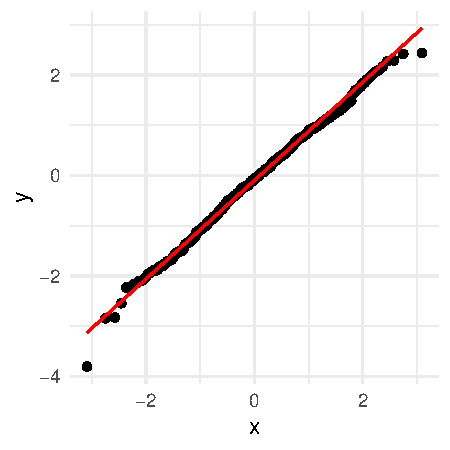
\includegraphics[width=\maxwidth]{img/mc-regression-05-a-1} 

}







\begin{enumerate}
\item [\textbf{A} \msquare] Die Annahme der normalverteilten Residuen ist nicht erfüllt. Die Punkte liegen zum überwiegenden Teil nicht auf der Geraden.
\item [\textbf{B} \msquare] Wir betrachten die Gerade, die durch die einzelnen Punkte laufen sollte. Wenn die 95\% der Punkte von der Geraden getroffen werden, dann gehen wir von normalverteilten Residuen aus.
\item [\textbf{C} \msquare] Die Annahme der normalverteilten Residuen ist erfüllt. Die Punkte liegen zum überwiegenden Teil nicht auf der Geraden und Korrelation ist negativ.
\item [\textbf{D} \msquare] Die Annahme der normalverteilten Residuen ist erfüllt. Die Punkte liegen zum überwiegenden Teil nicht auf der Geraden.
\item [\textbf{E} \msquare] Wir betrachten die Gerade und dabei insbesondere die beiden Enden der Gerade. Hier sollten die Punkte auf der Geraden liegen, dann ist die Annahme an die Normalverteilung der Residuen erfüllt. Diese Annahme ist nicht erfüllt.
\end{enumerate}

\section{Aufgabe \hfill (2 Punkte)}



Im Allgemeinen gibt es zwei mögliche Ziele für ein Regressionsmodell. Wir können eine Vorhersagemodell oder ein kausales Modell rechnen. Welche Aussage ist für ein prädiktives Modell richtig?



\begin{enumerate}
\item [\textbf{A} \msquare] Ein prädiktives Modell möchte die Zusammenhänge von X auf Y modellieren. Hierbei geht es um die Effekte von $X$ auf $Y$. Man sagt, wenn $x_1$ um 1 ansteigt ändert sich $Y$ um einen Betrag $\beta_1$.
\item [\textbf{B} \msquare] Wir modellieren den Zusammenhang zwischen $X$ und $Y$ wenn ein prädiktives Modell rerechnet wird. Dabei kann nicht der gesamte Datensatz genutzt werden. Es wird ein Trainingsdatensatz zum Trainieren des Modells benötigt.
\item [\textbf{C} \msquare] Ein prädiktives Modell wird auf einem Trainingsdatensatz trainiert und anschliessend über eine explorative Datenanalyse validiert. Signifikanzen über $\beta_i$ können hier nicht festgestellt werden.
\item [\textbf{D} \msquare] Ein prädiktives Modell basiert auf einem Traingsdatensatz und einem Testdatensatz. Auf dem Trainingsdatensatz wird das Modell trainiert und auf dem Testdatensatz validiert.
\item [\textbf{E} \msquare] Es wird ein Trainingsdatensatz zum Modellieren des Trainingsmodells benötigt. Der Testdatensatz dient rein zur Visualisierung. Dies gilt vor allem für ein prädiktives Modell.
\end{enumerate}

\section{Aufgabe \hfill (2 Punkte)}



Sie rechnen eine linearen Regression und erhalten folgende Abbildung der Residuen (\texttt{.resid}). Welche Aussage ist richtig?



{\centering 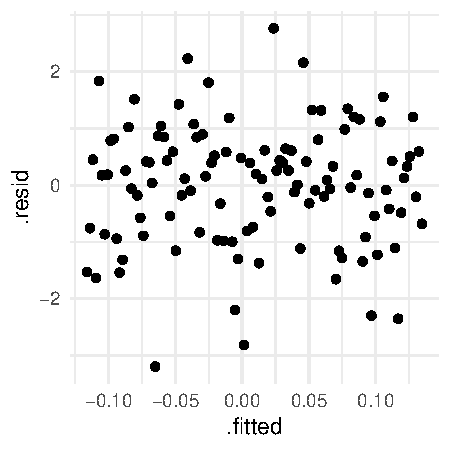
\includegraphics[width=\maxwidth]{img/mc-regression-06-a-1} 

}







\begin{enumerate}
\item [\textbf{A} \msquare] Die Annahme der normalverteilten Residuen ist erfüllt. Die Punkte liegen zum überwiegenden Teil auf der Diagonalen. Damit ist das Modell erfolgreich geschätzt worden.
\item [\textbf{B} \msquare] Wenn wir die Nulllinie betrachten so liegen die Punkte nicht gleichmäßig über und unter der Nulllinie. Unser Modell erfüllt nicht die Annahme von normalverteilten Residuen mit einem Mittelwert von 0 und einer Streuung von $s^2$.
\item [\textbf{C} \msquare] Die Annahme der normalverteilten Residuen ist erfüllt. Es ist ein Muster zu erkennen und wir können damit auf die Signifkanz von $x_1, ..., x_p$ schließen.
\item [\textbf{D} \msquare] Die Annahme der normalverteilten Residuen ist erfüllt. Kein Muster ist zu erkennen und keine Outlier zu beobachten.
\item [\textbf{E} \msquare] Wenn wir die Nulllinie betrachten so müssen die Punkte gleichmäßig über der Nulllinie liegen. Unser Modell erfüllt somit nicht die Annahme von normalverteilten Residuen mit einem Mittelwert von $>0$ und einer Streuung von $s$.
\end{enumerate}

\section{Aufgabe \hfill (2 Punkte)}




In den Humanwissenschaften wird der Korrelationskoeffizienten $\rho$ sehr häufig verwendet. Daher ist es auch wichtig für andere Forschende den Korrelationskoeffizienten $\rho$ zu verstehen. Welche Aussazu zu dem Korrelationskoeffizienten $\rho$ ist richtig?




\begin{enumerate}
\item [\textbf{A} \msquare] Korrelationskoeffizienten $\rho$ liegt zwischen 0 und 1. Darüber hinaus ist der Korrelationskoeffizienten $\rho$ einheitslos und kann als Standardisierung verstanden werden.
\item [\textbf{B} \msquare] Der Korrelationskoeffizienten $\rho$ ist eine standardisierte, statistische Maßzahl, die zwischen -1 und 1 liegt. Dabei ist Korrelationskoeffizienten $\rho$ einheitslos.
\item [\textbf{C} \msquare] Der Korrelationskoeffizienten $\rho$ wird wie das $\eta^2$ aus der ANOVA interpretiert. Der Korrelationskoeffizienten $\rho$ beschreibt den Anteil an erklärter Varianz durch die Regression. Dabei gibt er jedoch eine Richtung an und kann auch negativ werden.
\item [\textbf{D} \msquare] Der Korrelationskoeffizienten $\rho$ ist eine standardisierte, statistische Maßzahl, die zwischen 0 und 1 liegt. Dabei ist Korrelationskoeffizienten $\rho$ einheitslos. Eine Signifikanz kann nicht nachgewiesen werden.
\item [\textbf{E} \msquare] Der Korrelationskoeffizienten $\rho$ ist eine veraltete Darstellungsform von Effekten in der linearen Regression und wird wie das $\eta^2$ aus der ANOVA interpretiert. Der Korrelationskoeffizienten $\rho$ beschreibt den Anteil an erklärter Varianz durch die Regression.
\end{enumerate}

\section{Aufgabe \hfill (2 Punkte)}



Nach einer simplen linearen Regression zur Untersuchung vom Einfluss der $Fe_3O_4$-Konzentration in [$\mu g$] im Wasser auf das Trockengewicht von Wasserlinsen in [$kg$] erhalten Sie einen $\beta_{Fe_3O_4}$ Koeffizienten von $7.4\times 10^{-6}$ und einen hoch signifikanten $p$-Wert mit $0.00032$. Warum sehen Sie so einen kleinen Effekt bei einer so deutlichen Signifikanz?




\begin{enumerate}
\item [\textbf{A} \msquare] Das Gewicht und die $Fe_3O_4$-Konzentration korrelieren sehr stark, deshalb wird der $\beta_{Fe_3O_4}$ Koeffizient sehr klein. Mit einer ANOVA kann für die Korrelation korrigiert werden und der Effektschätzer passt dann zum p-Wert.
\item [\textbf{B} \msquare] Die Einheit der $Fe_3O_4$-Konzentration ist zu klein gewählt. Dadurch sehen wir den sehr kleinen $p$-Wert. Der $p$-Wert und die Einheit von der $Fe_3O_4$-Konzentration hängen antiproportional zusammen.
\item [\textbf{C} \msquare] Die Fallzahl ist zu klein angesetzt. Je kleiner die Fallzahl ist, desto höher ist die Teststatsitik und damit auch der $p$-Wert kleiner. Wir brauchen also mehr Fallzahl um den geringen Effekt noch signifikant zu krigen.
\item [\textbf{D} \msquare] Wenn der Effekt $\beta_{Fe_3O_4}$ winzig ist, dann kann es an einer falsch gewählten Einheit liegen. Der Anstieg von einer Einheit in $X$ führt ja zu einer Änderung von $\beta_{Fe_3O_4}$ in $x$. Wir müssen daher die Einheit von $y$ entsprechend anpassen.
\item [\textbf{E} \msquare] Manchmal ist die Einheit der Einflussvariable $X$ zu klein gewählt, so dass der Ansteig von 1 Einheit in $X$ zu einer zu kleinen Änderung in $y$ führt. Daher kann der Effekt $\beta_{Fe_3O_4}$ sehr klein wirken, aber auf einer anderen Einheit sehr viel größer sein. Der p-Wert wird auf einer einheitslosen Teststatistik bestimmt.
\end{enumerate}

\section{Aufgabe \hfill (2 Punkte)}



Neben der klassischen Regression kann die Funktion \texttt{lm()} in \Rlogo auch für welche andere Art von Anwendung genutzt werden?





\begin{enumerate}
\item [\textbf{A} \msquare] Die Funktion \texttt{lm()} berechnet die Varianzstruktur für eine ANOVA. Dannach kann dann über eine explorative Datenalayse nochmal eine Signifikanz berechnet werden. Sollte vor der Verwendung der Funktion \texttt{lm()} schon eine EDA gerechnet worden sein, so ist die Analyse wertlos.
\item [\textbf{B} \msquare] Die Funktion \texttt{lm()} in \Rlogo ist der letzte Schritt für einen Gruppenvergleich. Vorher kann eine ANOVA oder aber ein multipler Vergleich in \{emmeans\} gerechnet werden. In der Funktion  \texttt{lm()} werden die Gruppenvarianzen bestimmt.
\item [\textbf{C} \msquare] Ist die Einflussvariable $X$ numerisch so werden die Gruppenmittelwerte geschätzt und eine anschließende ANOVA sowie multipler Gruppenvergleich mit \{emmeans\} ist möglich.
\item [\textbf{D} \msquare] Neben der klassichen Verwendung der Funktion \texttt{lm()} in der linearen Regression kann auch ein Gruppenvergleich gerechnet werden. Dafür müssen aber alle Faktoren aus den Daten entfernt und numerishc umgewandelt werden. Dann kann das R Paket \{emmeans\} genutzt werden um die Korrelation zu berechnen. Eine Adjustierung ist dann nicht mehr notwendig.
\item [\textbf{E} \msquare] Die Funktion \texttt{lm()} in \Rlogo wird klassischerweise für die lineare Regression genutzt. Ist die Einflussvariable $X$ ein Faktor so werden die Gruppenmittelwerte geschätzt und eine anschließende ANOVA sowie multipler Gruppenvergleich mit \{emmeans\} ist möglich.
\end{enumerate}

\section{Aufgabe \hfill (2 Punkte)}



Wenn Ihr gemessener Endpunkt nicht einer Normalverteilung folgt, so können Sie dennoch Ihre Daten modellieren. Hierzu nutzen Sie dann das \textit{generalisierte lineare Modell (GLM)}. Welche Aussage ist richtig?




\begin{enumerate}
\item [\textbf{A} \msquare] Dank dem \textit{generalisierten linearen Modell (GLM)} können auch andere Verteilungsfamilien als die Normalverteilung mit einer linearen Regression modelliert werden.
\item [\textbf{B} \msquare] In \Rlogo ist mit dem \textit{generalisierten linearen Modell (GLM)} eine Modellierung implementiert, die die Poissonverteilung für Zähldaten oder die Binomialverteilung für 0/1-Daten modellieren kann. Weitere Modellierungen sind in \Rlogo auch mit zusätzlich geladenen Paketen nicht möglich.
\item [\textbf{C} \msquare] Das GLM ist ein faktisch maschineller Lernalgorithmus, der selstständig die Verteilungsfamilie für Y wählt.
\item [\textbf{D} \msquare] Das \textit{generalisierte lineare Modell (GLM)} erlaubt auch weitere Verteilungsgruppen für das $X$ bzw. die Einflussvariablen in einer linearen Regression zu wählen.
\item [\textbf{E} \msquare] Das GLM ist eine Vereinfachung des LM in R. Mit dem GLM lassen sich polygonale Regressionen rechnen. Somit stehen neben der Normalverteilung noch weitere Verteilungen zu Verfügung.
\end{enumerate}

\section{Aufgabe \hfill (2 Punkte)}



Sie führen ein Experiment zur Behandlung von Klaueninfektionen bei Schafe durch. Bei 3 Tieren finden Sie eine Erkrankung der Klauen vor und 8 Tiere sind gesund. Welche Aussage über den Effektschätzer Odds ratio ist richtig?



\begin{enumerate}
\item [\textbf{A} \msquare] Das Verhältnis von Chancen Odds ratio ergibt ein Chancenverhältnis von 0.38.
\item [\textbf{B} \msquare] Da es sich um ein Chancenverhältnis handelt ergibt sich ein Odds ratio von 3.67.
\item [\textbf{C} \msquare] Es ergibt sich ein Odds ratio von 0.27, da es sich um eine Chancenverhältnis handelt.
\item [\textbf{D} \msquare] Das Verhältnis der Chancen Odds ratio ergibt ein Chancenverhältnis von 0.27. Wir sind an der Chance krank zu sein interessiert.
\item [\textbf{E} \msquare] Der Anteil der Kranken wird berechnet. Da es sich um ein Anteil handelt ergibt sich ein Odds ratio von 0.27.
\end{enumerate}
    
% -----------------------------------------------------------------------
\clearpage
% -----------------------------------------------------------------------
\part{Programmieren in R}
% -----------------------------------------------------------------------

\section{Aufgabe \hfill (9 Punkte)}



 
%% --------------------------------------------------------------------
\begin{minipage}[t]{0.5\textwidth}

\includegraphics[width = 1.3cm]{/Users/kruppajo/work/GitHub/exam/avatare/Mark.png}
\end{minipage}
\begin{minipage}[t]{0.5\textwidth}
\hfill
\href{https://www.youtube.com/playlist?list=PLe51bCp9JvEFUnFqaJG5aRmON9i1ZbOYC}{
\includegraphics[width = 2cm]{img/youtube}}
\end{minipage}
\vspace{-3ex}
%% --------------------------------------------------------------------



\paragraph{Grundlegende Kenntnisse der Programierung in \Rlogo}

'Unter den Blinden ist der Einäuge König!', ruft Ihnen Mark entgegen. Leider kennt sich Mark überhaupt nicht mit den Grundlagen in \Rlogo aus aber sein Betreuer möchte gerne, dass die Auswertung in \Rlogo gemacht wird. Da müssen Sie dann wohl mal ran und helfen.\\[1Ex]

Mark: \textit{Was ist der Unterschied zwischen \texttt{library()} und \texttt{Packages} und warum brauche ich sowas in \Rlogo?} \textbf{(1 Punkt)}\\[1ex]
Sie antworten:\\[2Ex]

Mark: \textit{Jetzt lese ich hier von einem Faktor. Was ist ein Faktor in \Rlogo?} \textbf{(1 Punkt)}\\[1ex]
Sie antworten:\\[2Ex]

Mark: \textit{In R hat sich doch mein Datensatz geändert. Warum ist er jetzt wieder so wie vorher, wenn ich den Datensatz wieder aufrufe? Was mache ich falsch?} \textbf{(1 Punkt)}\\[1ex]
Sie antworten:\\[2Ex]

Mark: \textit{Warum brauche ich eigentlich das RStudio und R? Wo ist denn da der Unterschied?} \textbf{(1 Punkt)}\\[1ex]
Sie antworten:\\[2Ex]

Mark: \textit{Jetzt sehe ich wieder diese Tilde ($\sim$) in R. Wo brauchen wir diese denn nochmal?} \textbf{(1 Punkt)}\\[1ex]
Sie antworten:\\[2Ex]

Mark: \textit{In R gibt es Objekte, Wörter und Funktionen. Wie unterscheiden sich diese voneinander?} \textbf{(1 Punkt)}\\[1ex]
Sie antworten:\\[2Ex]

Mark: \textit{Wie sieht der Zuweisungs-Operator aus und was ist seine Funktion? Gerne mit Beispiel!} \textbf{(1 Punkt)}\\[1ex]
Sie antworten:\\[2Ex]

Mark: \textit{Wie speichern wir in R intern Daten ab? Ich brauche nochmal den Namen der Funktion. Was sind den die Vorteile von dieser Art der Speicherung?} \textbf{(1 Punkt)}\\[1ex]
Sie antworten:\\[2Ex]

Mark: \textit{Wie heißen nochmal die beiden \Rlogo Pakete, die wir fast immer laden, wenn wir \Rlogo nutzen wollen?} \textbf{(1 Punkt)}\\[1ex]
Sie antworten:\\[2Ex] 
\clearpage
% -----------------------------------------------------------------------

\section{Aufgabe \hfill (9 Punkte)}



 
%% --------------------------------------------------------------------
\begin{minipage}[t]{0.5\textwidth}

\includegraphics[width = 1.3cm]{/Users/kruppajo/work/GitHub/exam/avatare/Steffen.png}
\end{minipage}
\begin{minipage}[t]{0.5\textwidth}
\hfill
\href{https://www.youtube.com/playlist?list=PLe51bCp9JvEFUnFqaJG5aRmON9i1ZbOYC}{
\includegraphics[width = 2cm]{img/youtube}}
\end{minipage}
\vspace{1ex}
%% --------------------------------------------------------------------



\paragraph{Fortgeschrittene Kenntnisse der Programierung in \Rlogo}

'Hm...am Ende ist dann \Rlogo eigentlich gar nicht so schwer, wenn ich Hilfe habe.', meint  Steffen stolz und lacht Sie an. Nur leider kennt er sich überhaupt nicht mit \Rlogo aus! Das heißt, Sie müssen hier einmal Rede und Antwort stehen und helfen. Sonst wird es für Steffen dann in seinem Projektbericht nichts mit der Auswertung und Abgabe. Das kann auch keine Lösung für Steffen und Sie sein. Immerhin haben Sie schon so viel gelernt.\\[1Ex]

Steffen fragt: \textit{Wie nennt sich das Datenformat in R? Bitte mit kurzem Beispiel! \textbf{(1 Punkt)}}\\[1ex]
Sie antworten:\\[2Ex]

Steffen fragt: \textit{Warum wurden jeweils die R Pakete \texttt{\{emmeans\}}, \texttt{\{ggplot\}} und \texttt{\{readxl\}} geladen? \textbf{(2 Punkte)}}\\[1ex]
Sie antworten:\\[2Ex]

Steffen fragt: \textit{Man kann doch die Funktion \texttt{emmeans()} von Varianzhomogenität auf Varianzheterogenität umstellen. Wie ging das noch gleich? \textbf{(1 Punkt)}}\\[1ex]
Sie antworten:\\[2Ex]

Steffen fragt: \textit{Die Funktion \texttt{emmeans()} erlaubt es den Faktor $f_1$ getrennt in jedem Level des Faktors $f_2$ auszuwerten. Wie mache ich das? \textbf{(1 Punkt)}}\\[1ex]
Sie antworten:\\[2Ex]

Steffen fragt: \textit{Ich habe hier einen Gruppenvergleich als Expriment durchgeführt. Wenn ich jetzt die Daten in R reingeladen habe, was muss ich dann als erstes machen und warum nochmal? \textbf{(2 Punkte)}}\\[1ex]
Sie antworten:\\[2Ex]

Steffen fragt: \textit{Datumsangaben sind schwierig, da es nur ein gültiges Format gibt, was zwischen Programmen funktioniert. Wie lautet das Format? \textbf{(1 Punkt)}}\\[1ex]
Sie antworten:\\[2Ex]

Steffen fragt: \textit{Wie spezifizieren wir nochmal eine Interaktion in einem Modell mit zwei Faktoren $f_1$ und $f_2$? \textbf{(1 Punkt)}}\\[1ex]
Sie antworten:\\[2Ex]



 
\clearpage
% -----------------------------------------------------------------------
\part{Deskriptive Statistik \& Explorative Datenanalyse}
% -----------------------------------------------------------------------

%% --------------------------------------------------------------------
\begin{flushright}
\tiny
bla
blub
\end{flushright}
%% --------------------------------------------------------------------

\section{Aufgabe \hfill (8 Punkte)}

\textit{Geben Sie grundsätzlich Formeln und Rechenweg zur Lösung der Teilaufgaben mit an!} \\[1Ex]
 

 
%% --------------------------------------------------------------------
\begin{minipage}[t]{0.5\textwidth}

\includegraphics[width = 1.3cm]{/Users/kruppajo/work/GitHub/exam/avatare/Yuki.png}
\end{minipage}
\begin{minipage}[t]{0.5\textwidth}
\hfill
\href{https://youtu.be/t0WYa_LVc5o}{
\includegraphics[width = 2cm]{img/youtube}}
\end{minipage}
\vspace{-3ex}
%% --------------------------------------------------------------------



\paragraph{Zerforschen des Barplots}

Yuki steht vor einem ersten Problem, denn wenn es nach seiner Betreuer geht, soll er in einem einem Gewächshausexperiment Lauch auswertet. Soweit eigentlich alles passend. Besser wäre was anderes gewesen. Orchideen. Ein wunderbares Hobby um sich drin zu verlieren und Abstand zu bekommen. Yuki denkt gerne über Orchideen nach. Das heißt erstmal überlegen für Yuki. 'Hm...', Reese's Peanut Butter Cups und London Grammar. Das ist und bleibt die beste Kombination zum Nachdenken für Yuki. Die Behandlung werden verschiedene Lüftungssysteme und Folientunnel ($ctrl$, $storm$ und $tornado$) sein. In seiner Exceldatei wird er den Messwert ($Y$) \textit{Frischegewicht} als \textit{freshmatter} aufnehmen. Vorab soll Yuki aber eimal die folgenden Barplots seiner Betreuer nachbauen, damit er den \Rlogo Code schonmal für später vorliegen hat. Damit geht das Problem schon los. Yuki und die Faulheit, eine unendliche Geschichte mit kniffeligen Wendungen.



{\centering 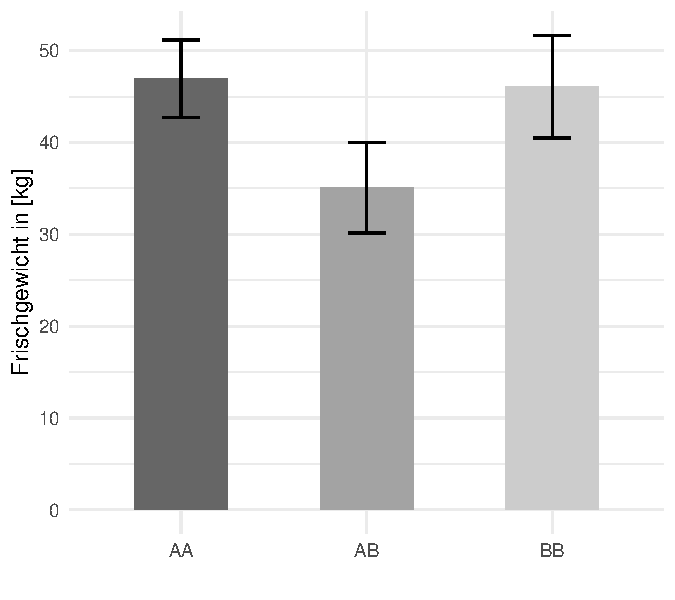
\includegraphics[width=\maxwidth]{img/barplot-02-1} 

}




Leider kennt sich Yuki mit der Erstellung von Barplots in \Rlogo nicht aus. Deshalb braucht er bei der Visualisierung Ihre Hilfe!

\begin{enumerate}
\item Formulieren Sie die wissenschaftliche Fragestellung! \textbf{(1 Punkt)}
\item Erstellen Sie eine Tabelle mit den statistischen Maßzahlen der drei Barplots! \textit{Beachten Sie die korrekte Darstellungsform der statistischen Maßzahlen!} \textbf{(3 Punkte)}
\item Erstellen Sie einen beispielhaften Datensatz im \Rlogo üblichen Format, aus dem die drei Barplots \textit{möglicherweise} erstellt wurden! \textbf{(2 Punkte)}
\item Kann Yuki einen Unterschied zwischen den Behandlungen erwarten? Begründen Sie Ihre Antwort! \textbf{(2 Punkte)}
\end{enumerate} 
\clearpage
% -----------------------------------------------------------------------

\section{Aufgabe \hfill (8 Punkte)}

\textit{Geben Sie grundsätzlich Formeln und Rechenweg zur Lösung der Teilaufgaben mit an!} \\[1Ex]
 

 
%% --------------------------------------------------------------------
\begin{minipage}[t]{0.5\textwidth}

\includegraphics[width = 1.3cm]{/Users/kruppajo/work/GitHub/exam/avatare/Paula.png}
\end{minipage}
\begin{minipage}[t]{0.5\textwidth}
\hfill
\href{https://youtu.be/vXnLttRL_VI}{
\includegraphics[width = 2cm]{img/youtube}}
\end{minipage}
\vspace{-3ex}
%% --------------------------------------------------------------------



\paragraph{Visualisierung des Barplots}


Paula steht vor einem ersten Problem, denn wenn es nach ihrer Betreuerin geht, soll sie in einem einem Gewächshausexperiment Kartoffeln auswertet. Soweit eigentlich alles passend. Besser wäre was anderes gewesen. Harry Potter. Ein wunderbares Hobby um sich drin zu verlieren und Abstand zu bekommen. Paula denkt gerne über Harry Potter nach. Die Behandlung waren verschiedene Lichtstufen ($none$, $200lm$ und $600lm$). In ihrer Exceldatei hat sie den Endpunkt ($Y$) \textit{Ertrag} als \textit{yield} aufgenommen. Nun soll Paula die Daten eimal als Barplots in einer Präsentation visualisieren, damit ihrer Betreuerin wieder klar wird, was sie eigentlich nochmal gemacht hat und was für ein Ergbnis in einem statistischen Test zu erwarten wäre. Wäre da nicht noch etwas. Paula und der Perfektionismus, eine unendliche Geschichte mit kniffeligen Wendungen. Aber egal. Einfach mal raus um zu Fechten. Ohne Ziel und Uhr. Das ist was für Paula.

\begin{table}[!h]
\centering
\begin{tabular}{cc}
\toprule
treatment & yield\\
\midrule
200lm & 30.8\\
600lm & 50.6\\
600lm & 35.5\\
none & 53.9\\
600lm & 52.5\\
\addlinespace
200lm & 19.3\\
600lm & 53.0\\
none & 49.5\\
none & 29.6\\
200lm & 44.5\\
\addlinespace
600lm & 36.5\\
200lm & 35.2\\
none & 39.7\\
none & 40.1\\
\bottomrule
\end{tabular}
\end{table}



Leider kennt sich Paula mit der Erstellung von Barplots nicht aus. Deshalb braucht sie bei der Visualisierung Ihre Hilfe!

\begin{enumerate}
\item Formulieren Sie die wissenschaftliche Fragestellung! \textbf{(1 Punkt)}
\item Zeichnen Sie in \textit{einer} Abbildung die Barplots für die Behandlung von Kartoffeln! Beschriften Sie die Achsen entsprechend!\textbf{(4 Punkte)}
\item Beschriften Sie \textit{einen} Barplot mit den gängigen statistischen Maßzahlen! \textbf{(2 Punkte)}
\item Wenn Paula \textit{keinen Effekt} zwischen den Behandlungen von Kartoffeln erwarten würde, wie sehen dann die Barplots aus? \textit{Antworten Sie mit einer Skizze der Barplots!}
  \textbf{(1 Punkt)}
\end{enumerate} 
\clearpage
% -----------------------------------------------------------------------

\section{Aufgabe \hfill (9 Punkte)}

\textit{Geben Sie grundsätzlich Formeln und Rechenweg zur Lösung der Teilaufgaben mit an!} \\[1Ex]
 

 
%% --------------------------------------------------------------------
\begin{minipage}[t]{0.5\textwidth}

\includegraphics[width = 1.3cm]{/Users/kruppajo/work/GitHub/exam/avatare/Jonas.png}
\end{minipage}
\begin{minipage}[t]{0.5\textwidth}
\hfill
\href{https://youtu.be/Xf0yE-o7bEU}{
\includegraphics[width = 2cm]{img/youtube}}
\end{minipage}
\vspace{-3ex}
%% --------------------------------------------------------------------



\paragraph{Zerforschen des Boxplots}

Jonas und die Erschöpfung, eine unendliche Geschichte mit kniffeligen Wendungen. Deshalb gilt anschauen, was andere vor einem gemacht haben. Für Jonas ist es eine Möglichkeit schneller ans Ziel zu gelangen. Jonas soll in seiner Hausarbeit Lauch untersuchen. Die Behandlung in seiner Hausarbeit werden verschiedene Düngestufen ($ctrl$, $low$ und $high$) sein. Erheben wird Jonas als Endpunkt ($Y$) \textit{Ertrag} benannt als \textit{yield} in seiner Exceldatei. Von seiner Betreuerin erhält er nun folgende Abbildung von Boxplots, die er erstmal zur Übung nachbauen soll, bevor er mit dem eigentlichen Versuch beginnt. Aber nur in passender Atmospäre! Schon dutzende Male gesehen: Mission Impossible. Aber immer noch großartig zusammen mit Snickers.



{\centering 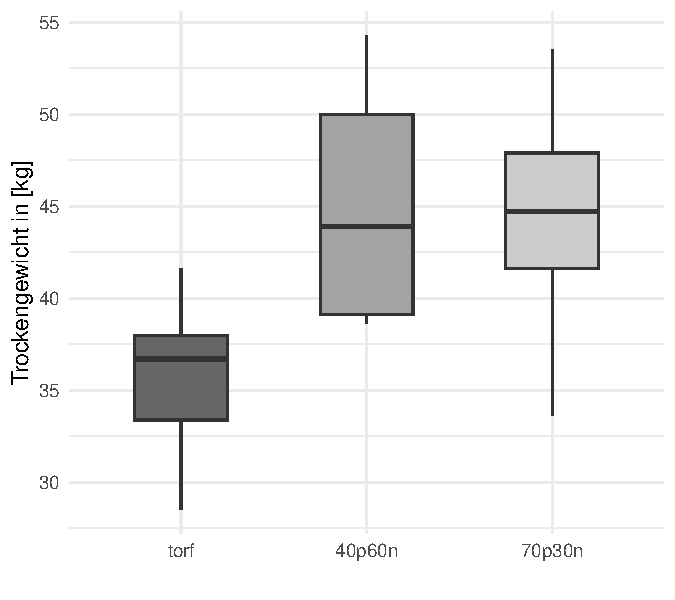
\includegraphics[width=\maxwidth]{img/boxplot-02-zer-1} 

}




Leider kennt sich Jonas mit der Erstellung von Boxplots in \Rlogo nicht aus. Deshalb braucht er bei der Visualisierung Ihre Hilfe!

\begin{enumerate}
\item Erstellen Sie eine Tabelle mit den statistischen Maßzahlen aus der obigen Abbildung der drei Boxplots! \textit{Beachten Sie die korrekte Darstellungsform der statistischen Maßzahlen!} \textbf{(3 Punkte)}
\item Beschriften Sie \textit{einen} der Boxplots mit den gängigen statistischen Maßzahlen! \textbf{(2 Punkte)}
\item Erstellen Sie einen beispielhaften Datensatz, aus dem die drei Boxplots \textit{möglicherweise} erstellt wurden, im \Rlogo üblichen Format! \textbf{(2 Punkte)}
\item Kann Jonas einen Unterschied zwischen den Behandlungen erwarten? Begründen Sie Ihre Antwort! \textbf{(2 Punkte)}
\end{enumerate} 
\clearpage
% -----------------------------------------------------------------------

\section{Aufgabe \hfill (9 Punkte)}

\textit{Geben Sie grundsätzlich Formeln und Rechenweg zur Lösung der Teilaufgaben mit an!} \\[1Ex]
 

 
%% --------------------------------------------------------------------
\begin{minipage}[t]{0.5\textwidth}

\includegraphics[width = 1.3cm]{/Users/kruppajo/work/GitHub/exam/avatare/Yuki.png}
\end{minipage}
\begin{minipage}[t]{0.5\textwidth}
\hfill
\href{https://youtu.be/0xc0jIPeiyw}{
\includegraphics[width = 2cm]{img/youtube}}
\end{minipage}
\vspace{-3ex}
%% --------------------------------------------------------------------



\paragraph{Visualisierung des Boxplots}

Boxplots sind bedeutend in der Darstellung von wissenschaftlichen Ergebnissen. Leider hat sich Yuki nicht gemerkt, welche statistischen Maßzahlen für einen Boxplot erhoben werden müssen. Besser wäre was anderes gewesen. Yuki liebt Orchideen. Darin kann er sich wirklich verlieren und immer wieder neu begeistern. Das ist in soweit doof, da nach seiner Betreuerin nun Boxplots aus seinen Daten gebaut werden sollen, bevor es mit dem statistischen Testen weitergeht. Anhand von Boxplots lässt sich eine Aussage über die Varianzhomogenität über die Behandlungsgruppen treffen. Die Behandlung für Brokoli waren verschiedene Lüftungssystemen und Folientunneln ($ctrl$ und $tornado$). Erfasst wurde von Yuki als Outcome ($Y$) \textit{Frischegewicht}. Yuki hat dann \textit{freshmatter} in seiner Exceldatei eintragen. Aber nur in passender Atmospäre! Hm, lecker Reese's Peanut Butter Cups und dazu dann im Hintergrund Matrix laufen lassen.

\begin{table}[!h]
\centering
\begin{tabular}{cc}
\toprule
treatment & drymatter\\
\midrule
ctrl & 57.9\\
tornado & 22.7\\
tornado & 23.6\\
ctrl & 38.0\\
ctrl & 48.2\\
\addlinespace
tornado & 33.8\\
tornado & 23.5\\
ctrl & 53.8\\
tornado & 22.3\\
tornado & 24.7\\
\addlinespace
ctrl & 47.2\\
ctrl & 39.6\\
tornado & 28.4\\
tornado & 29.1\\
ctrl & 55.1\\
\bottomrule
\end{tabular}
\end{table}



Leider kennt sich Yuki mit der Erstellung von Boxplots nicht aus. Deshalb braucht er bei der Visualisierung Ihre Hilfe!

\begin{enumerate}
\item Zeichnen Sie in \textit{einer} Abbildung die beiden Boxplots für die zwei Behandlungen von Brokoli! Beschriften Sie die Achsen entsprechend! \textbf{(5 Punkte)} 
\item Wie ist Ihr Vorgehen, wenn Sie eine \textit{gerade} Anzahl an
  Beobachtungen pro Gruppe haben? \textbf{(1 Punkt)}
\item Beschriften Sie \textit{einen} der beiden Boxplots mit den gängigen
  statistischen Maßzahlen! \textbf{(2 Punkte)}
\item Wenn Sie \textit{keinen Effekt} zwischen den Behandlungen von
  Brokoli erwarten würden, wie sehen dann die beiden Boxplots aus?
  \textit{Antworten Sie mit einer Skizze der Boxplots!}
  \textbf{(1 Punkt)}
\end{enumerate} 
\clearpage
% -----------------------------------------------------------------------

\section{Aufgabe \hfill (8 Punkte)}

\textit{Geben Sie grundsätzlich Formeln und Rechenweg zur Lösung der Teilaufgaben mit an!} \\[1Ex]
 

 
%% --------------------------------------------------------------------
\begin{minipage}[t]{0.5\textwidth}

\includegraphics[width = 1.3cm]{/Users/kruppajo/work/GitHub/exam/avatare/Mark.png}
\end{minipage}
\begin{minipage}[t]{0.5\textwidth}
\hfill
\href{https://youtu.be/aXvxGC4YLqk}{
\includegraphics[width = 2cm]{img/youtube}}
\end{minipage}
\vspace{-3ex}
%% --------------------------------------------------------------------



\paragraph{Visualisierung des Histogramm für kategoriale Daten}

Mark schmeißt noch eine Handvoll Marzipankugeln in seinen Rachen. Im Hintergrund klirrt leise der Spiegel zum Sound von Andrea Berg. Mark betrachtet die folgenden Daten nach einem Stallexperiment mit Zandern. In dem Experiment wurden die Anzahl an weißen Blutkörperchen gezählt. Nach der Meinung seiner Betreuerin muss als erstes geschaut werden, wie diese verteilt sind. Also welcher statistischen Verteilung die Anzahl an weißen Blutkörperchen folgen. Dazu soll Mark ein Histogramm verwenden. Dann hätte man auch einen guten Überblick über das Outcome ($Y$). Es wäre einfacher, wenn da nicht noch was wäre. Mark und die Unsicherheit, eine unendliche Geschichte mit kniffeligen Wendungen. Mark streichelt liebevoll der Hamster. Der Kopf ist in seinem Schloß vergraben um den Klang von Andrea Berg zu dämpfen.

\begin{center}
Die Anzahl an weißen Blutkörperchen: 3, 6, 4, 2, 8, 1, 8, 4, 2, 5, 5, 2, 0, 4, 5, 3, 3, 8, 3, 4, 5, 1, 5, 2, 5, 6, 4, 4, 4, 6
\end{center}

Leider kennt sich Mark mit der Erstellung von Histogrammen überhaupt nicht aus. Deshalb braucht er bei der Erstellung Ihre Hilfe!

\begin{enumerate}
\item Zeichen Sie ein Histogramm um die Verteilung der Daten zu visualisieren! (\textbf{3 Punkte})
\item Beschriften Sie die Achsen der Abbildung! (\textbf{2 Punkte})
\item Ergänzen Sie die absoluten und relativen Häufigkeiten in der
  Abbildung! \textbf{(1 Punkt)}
\item Berechnen Sie aus den Daten die \textit{Wahrscheinlichkeit}
  gleich oder mehr als die Anzahl 5 zu beobachten! \textbf{(1
    Punkt)}
\item Berechnen Sie aus den Daten die \textit{Chance} gleich oder mehr
  als die Anzahl 5 zu beobachten! \textbf{(1 Punkt)}
\end{enumerate}

 
\clearpage
% -----------------------------------------------------------------------

\section{Aufgabe \hfill (8 Punkte)}

\textit{Geben Sie grundsätzlich Formeln und Rechenweg zur Lösung der Teilaufgaben mit an!} \\[1Ex]
 

 
%% --------------------------------------------------------------------
\begin{minipage}[t]{0.5\textwidth}

\includegraphics[width = 1.3cm]{/Users/kruppajo/work/GitHub/exam/avatare/Jonas.png}
\end{minipage}
\begin{minipage}[t]{0.5\textwidth}
\hfill
\href{https://youtu.be/ORHSPTCdfeY}{
\includegraphics[width = 2cm]{img/youtube}}
\end{minipage}
\vspace{-3ex}
%% --------------------------------------------------------------------



\paragraph{Visualisierung des Histogramm für kontinuierliche Daten}

In einem Gespräch mit seiner Betreuerin wird Jonas gebeten seine Daten aus einem Feldexperiment mit Maiss in einem Histogramm darzustellen. Aus den Boxen wummert Iron Maiden und sein Mund ist verklebt von Snickers. 'Herrlich', denkt Jonas. In seinem Experiment hat er die mittleren Läsionen auf den Blättern erst fotographiert und dann ausgezählt. Laut seiner Betreuerin soll das Histogramm helfen, die Verteilung der die mittleren Läsionen auf den Blättern zu bestimmen.  Es wäre einfacher, wenn da nicht noch was wäre. Jonas und die Erschöpfung, eine unendliche Geschichte mit kniffeligen Wendungen. Jonas streichelt liebevoll das Meerschweinchen. Der Kopf ist in seinem Schloß vergraben um den Klang von Iron Maiden zu dämpfen.

\begin{center}
Die mittleren Läsionen auf den Blättern: 8.8, 9.8, 7.3, 10.6, 12.5, 13.4, 9.2, 11.1, 8.8, 9.2, 13.2, 8.6, 13.6, 9.3, 9.3, 12.5, 11, 7.1, 7, 7.7, 9.9, 10.5
\end{center}

Leider kennt sich Jonas mit der Erstellung von Histogrammen überhaupt nicht aus. Deshalb braucht er bei der Erstellung Ihre Hilfe!

\begin{enumerate}
\item Zeichen Sie ein Histogramm um die Verteilung der Daten zu visualisieren! (\textbf{3 Punkte})
 \item Erläutern Sie Ihr Vorgehen um ein Histogramm für kontinuierliche Daten zu zeichnen!  (\textbf{2 Punkte})
\item Beschriften Sie die Achsen der Abbildung! (\textbf{2 Punkte})
\item Ergänzen Sie die relativen Häufigkeiten in der Abbildung! \textbf{(1 Punkt)}  
\end{enumerate}

 
\clearpage
% -----------------------------------------------------------------------

\section{Aufgabe \hfill (10 Punkte)}

\textit{Geben Sie grundsätzlich Formeln und Rechenweg zur Lösung der Teilaufgaben mit an!} \\[1Ex]
 

 
%% --------------------------------------------------------------------
\begin{minipage}[t]{0.5\textwidth}

\includegraphics[width = 1.3cm]{/Users/kruppajo/work/GitHub/exam/avatare/Paula.png}
\end{minipage}
\begin{minipage}[t]{0.5\textwidth}
\hfill
\href{https://youtu.be/VAqiUdV4WQ0}{
\includegraphics[width = 2cm]{img/youtube}}
\end{minipage}
\vspace{-3ex}
%% --------------------------------------------------------------------




\paragraph{Visualisierung des Scatterplots}

Paula liest laut: 'Wenn zwei kontinuierliche Variablen vorliegen, können diese in einer exploartiven Datenanalyse...'. Paula stoppt. 'Hm...', Smarties und White Lies. Das ist und bleibt die beste Kombination zum Nachdenken für Paula. Was waren noch gleich kontinuierliche Variablen? In ihrer Abschlussarbeit hatte sie einen Leistungssteigerungsversuch in der Uckermark durchgeführt. Dabei ging es um den Zusammenhang zwischen Protein/Fettrate [\%/kg] und mittlerer Eisenkonzentration [Fe/ml] im groben Kontext von Puten. Nun stellt sich die Frage für sie, ob es überhaupt einen Zusammenhang zwischen den gemessenen Variablen gibt. Dafür war eine explorative Datenanalyse gut! Paula und der Perfektionismus, eine unendliche Geschichte mit kniffeligen Wendungen. Dann was anderes. Das Verrückte ist, dass die Ratte Jagd auf roter Oktober wirklich liebt. Das ist Paula sehr recht, denn sie braucht Entspannung.

\begin{table}[!h]
\centering
\begin{tabular}{cc}
\toprule
Protein/Fettrate [\%/kg] & Mittlerer Eisenkonzentration [Fe/ml]\\
\midrule
24.7 & 28.6\\
19.3 & 24.7\\
21.0 & 27.3\\
32.2 & 40.2\\
25.4 & 31.2\\
\addlinespace
27.5 & 32.3\\
25.5 & 31.5\\
25.2 & 29.4\\
20.6 & 23.6\\
32.8 & 41.1\\
\addlinespace
25.0 & 33.4\\
27.7 & 36.3\\
\bottomrule
\end{tabular}
\end{table}



Leider kennt sich Paula mit der Erstellung einer explorativen Datenanalyse für kontinuierliche Daten überhaupt nicht aus. Deshalb braucht sie bei der Erstellung Ihre Hilfe!

\begin{enumerate}
\item Erstellen Sie eine Visualisierung für die Datentabelle. Beschriften Sie
  die Achsen entsprechend! \textbf{(4 Punkte)}
\item Schätzen Sie eine Gerade durch die Punkte! \textbf{(1 Punkt)}
\item Beschriften Sie die Gerade mit den gängigen statistischen Maßzahlen! Geben Sie die numerischen Zahlenwerte mit an! \textbf{(3 Punkte)}
\item Wenn \textit{kein} Effekt von $x$ auf $y$ vorhanden wäre, wie würde die Gerade verlaufen und welche Werte würden die statistischen Maßzahlen annehmen? \textbf{(2 Punkt)}
\end{enumerate} 
\clearpage
% -----------------------------------------------------------------------

\section{Aufgabe \hfill (10 Punkte)}

\textit{Geben Sie grundsätzlich Formeln und Rechenweg zur Lösung der Teilaufgaben mit an!} \\[1Ex]
 

 
%% --------------------------------------------------------------------
\begin{minipage}[t]{0.5\textwidth}

\includegraphics[width = 1.3cm]{/Users/kruppajo/work/GitHub/exam/avatare/Nilufar.png}
\end{minipage}
\begin{minipage}[t]{0.5\textwidth}
\hfill
\href{https://youtu.be/t_1KL77mfmg}{
\includegraphics[width = 2cm]{img/youtube}}
\end{minipage}
\vspace{-3ex}
%% --------------------------------------------------------------------



\paragraph{Visualisierung des Mosaicplots}

Zwei kategoriale Variablen darzustellen ist nicht so einfach. Nilufar hatte erst über einen Mittelwert nachgedacht, dann aber die Idee verworfen. Wäre da nicht noch was anderes. Wenn die Erwartung nicht wäre, ja dann wäre wohl vieles möglich für Nilufar! Aber so.. Dabei hatte sie sich in ein Kreuzungsexperiment im Teuteburgerwald zum einen die Behandlung Ökologisch [ja/nein] und zum anderen die Messung Protein/Fettrate im Zielbereich [ja/nein] im Kontext von Schweinen angeschaut. Jetzt möchte ihr Betreuer erstmal die langen Tabellen mit ja/nein in einer explorativen Datenanalyse zusammengefasst bekommen. Sonst geht es bei ihrem Projektbericht nicht weiter. Was super nervig ist. Nilufar will später nochmal raus um zu Kicken. Druck ablassen, dass muss sie auch.



\vspace{1Ex}

\begin{center}
\begin{minipage}[t]{0.45\textwidth}
%\small
\begin{center}

\begin{tabular}{p{2.5cm}p{2.5cm}p{2.5cm}p{2.5cm}}
\toprule
Ökologisch & Protein/Fettrate im Zielbereich\\
\midrule
ja & nein\\
ja & nein\\
nein & ja\\
ja & ja\\
nein & nein\\
\addlinespace
ja & nein\\
ja & nein\\
ja & ja\\
nein & nein\\
ja & ja\\
\addlinespace
ja & nein\\
nein & nein\\
nein & nein\\
nein & nein\\
\bottomrule
\end{tabular}


\end{center}
\end{minipage}
\begin{minipage}[t]{0.45\textwidth}
%\small
\begin{center}

\begin{tabular}{p{2.5cm}p{2.5cm}p{2.5cm}p{2.5cm}}
\toprule
Ökologisch & Protein/Fettrate im Zielbereich\\
\midrule
ja & ja\\
nein & ja\\
nein & ja\\
nein & nein\\
nein & ja\\
\addlinespace
nein & nein\\
nein & nein\\
ja & nein\\
nein & nein\\
ja & ja\\
\addlinespace
ja & nein\\
ja & nein\\
nein & ja\\
ja & nein\\
\bottomrule
\end{tabular}


\end{center}
\end{minipage}
\end{center}

\vspace{2Ex}

Leider kennt sich Nilufar mit der Erstellung einer explorativen Datenanalyse für kategoriale Daten überhaupt nicht aus. Deshalb braucht sie bei der Erstellung Ihre Hilfe!

\begin{enumerate}
\item Stellen Sie den Zusammenhang zwischen den beiden kategorialen Variablen in einer zusammenfassenden Tabelle dar! \textbf{(3 Punkte)}
\item Visualisieren Sie den Zusammenhang zwischen den beiden kategorialen Variablen! \textbf{(3 Punkte)}
\item Berechnen Sie die Verhältnisse in der Visualisierung! Welche Annahme haben Sie getroffen? \textbf{(2 Punkte)}
\item Wenn \textit{ein} Effekt von der Behandlung vorliegen würde, wie würde die Tabelle und die Visualisierung aussehen? \textbf{(2 Punkt)}
\end{enumerate} 
\clearpage
% -----------------------------------------------------------------------

\section{Aufgabe \hfill (10 Punkte)}

\textit{Geben Sie grundsätzlich Formeln und Rechenweg zur Lösung der Teilaufgaben mit an!} \\[1Ex]
 

 
%% --------------------------------------------------------------------
\begin{minipage}[t]{0.5\textwidth}

\includegraphics[width = 1.3cm]{/Users/kruppajo/work/GitHub/exam/avatare/Jessica.png}\hspace{-4mm}
\includegraphics[width = 1.3cm]{/Users/kruppajo/work/GitHub/exam/avatare/Tina.png}
\end{minipage}
\begin{minipage}[t]{0.5\textwidth}
\hfill
\href{https://youtu.be/Op-gjzASH9I}{
\includegraphics[width = 2cm]{img/youtube}}
\end{minipage}
%% --------------------------------------------------------------------



\paragraph{Visualisierung von Verteilungen}

'Was soll das denn jetzt schon wieder sein? Drei Boxplot, die auf der Seite liegen?', entfährt es Tina und schaut dabei Jessica an. 'Keine Ahnung. Es ist bestimmt wieder so ein Lernziel mit der Verteilung und so.', meint Jessica sichtlich genervt und mampft noch ein paar Schokobons. 'Du weißt doch wie es heißt, \textit{Frei ist, wer missfallen kann.}\footnote{Oschmann, A. (2024) Mädchen stärken: Stärken fördern, Selbstwert erhöhen und liebevoll durch Krisen begleiten. Goldegg Verlag}', merkt Tina nickend an. Die beiden schauen angestrengt auf die drei Boxplots. Das Ziel ist es zu verstehen, wie eine Verteilung anhand eines Boxplots bewertet werden kann. Jessica und der Mangel machen die Sache nicht einfacher.



{\centering 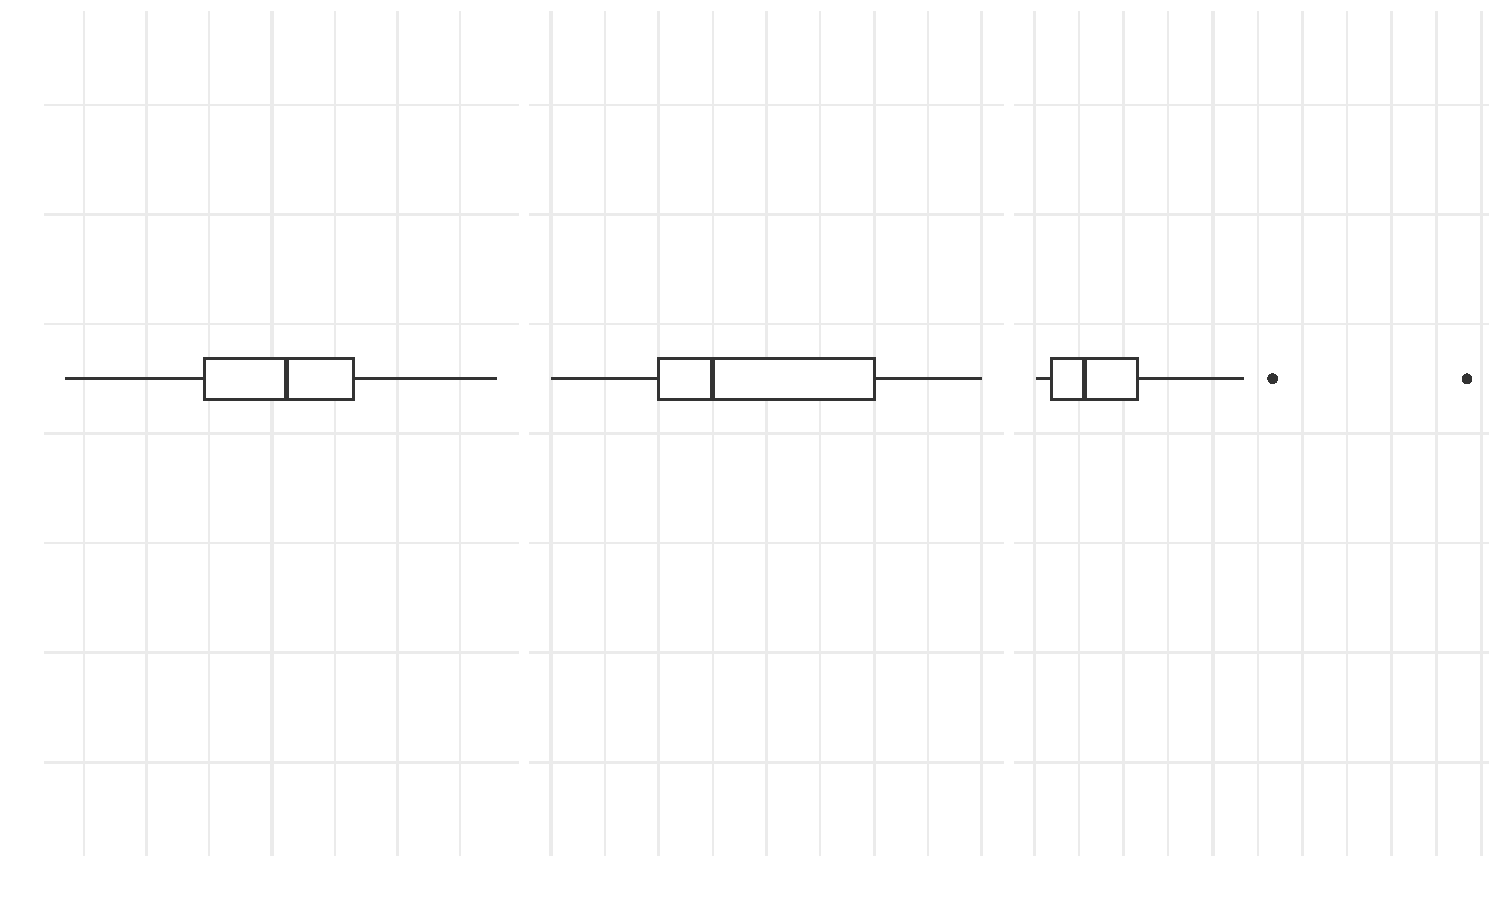
\includegraphics[width=\maxwidth]{img/desc-stat-11-1} 

}




Jetzt brauchen Tina und Jessica Ihre Hilfe bei der Abschätzung einer Verteilung anhand von Boxplots um ihre Arbeit dann in diesem Semester noch abschließen zu können.

\begin{enumerate}
\item Zeichnen Sie über die Boxplots die entsprechende zugehörige Verteilung! \textbf{(3 Punkte)} 
\item Zeichnen Sie unter die Boxplots die entsprechende zugehörige Beobachtungen als Stiche! \textbf{(3 Punkte)}
\item Wie viel Prozent der Beobachtungen fallen in das IQR? Ergänzen Sie die Abbildung entsprechend um den Bereich! \textbf{(2 Punkte)}
\item Wie viel Prozent der Beobachtungen fallen in $\bar{y} \pm 1s$ und $\bar{y} \pm 2s$  unter der Annahme einer Normalverteilung? \textbf{(2 Punkte)}
\end{enumerate} 
\clearpage
% -----------------------------------------------------------------------
\part{Statistisches Testen \& statistische Testtheorie}
% -----------------------------------------------------------------------  

\section{Aufgabe \hfill (9 Punkte)}


 
%% --------------------------------------------------------------------
\begin{minipage}[t]{0.5\textwidth}
\includegraphics[width = 1.3cm]{/Users/kruppajo/work/GitHub/exam/avatare/Jessica.png}\hspace{-4mm}\includegraphics[width = 1.3cm]{/Users/kruppajo/work/GitHub/exam/avatare/Yuki.png}
\end{minipage}
\begin{minipage}[t]{0.5\textwidth}
\hfill
\href{https://youtu.be/aHVYuFKTqZs}{\includegraphics[width = 2cm]{img/youtube}}
\end{minipage}
%% --------------------------------------------------------------------



\paragraph{Grundgesamtheit und experimentelle Stichprobe}

'Grundlage des statistischen Testen ist das Verständnis von der Grundgesamtheit (eng. \textit{population} oder \textit{ground truth}) und der experimentellen Stichprobe (eng. \textit{sample}). ', liest Yuki laut aus dem Skript vor. Jessica war kurz eingenickt und wird mit einem Stoß geweckt. 'Reiz dich zusammen und iss noch ein paar Reese's Peanut Butter Cups das hilft mir immer. Alleine komme ich hier nicht weiter.', tadelt Yuki Jessica etwas zu forsch. 'War ne lange Nacht', mault Jessica. Beide sollen in ihrer Abschlussarbeit einen statistischen Test interpretieren und versuchen die Grundlagen zu wiederholen. Jessica war auf einem Konzert von David Bowie.

\vspace{1ex}

Leider kennen sich Yuki und Jessica mit der Grundgesamtheit und der Stuchprobe überhaupt nicht aus. Daher sind Sie gefragt!

\begin{enumerate}
\item Nennen Sie das statistische Verfahren und zwei konkrete Beispiele zur Durchführung um von einer Grundgesamtheit auf eine Stichprobe zu gelangen! \textbf{(3 Punkte)}
\item Erklären Sie den Zusammenhang zwischen Stichprobe und Grundgesamtheit an einem Schaubild! Beschriften Sie das Schaubild entsprechend!
  \textit{Nutzen Sie hierfür als Veranschaulichung ein aussagekräftiges Beispiel!}  \textbf{(3 Punkte)}
\item Erweitern Sie das Schaubild um die Entstehung von $Pr(D|H_0)$! \textit{Nutzen Sie hierfür als Veranschaulichung ein aussagekräftiges Beispiel!}  \textbf{(3 Punkte)}
\end{enumerate} 
\clearpage
% -----------------------------------------------------------------------

\section{Aufgabe \hfill (9 Punkte)}


 
%% --------------------------------------------------------------------
\begin{minipage}[t]{0.5\textwidth}
\includegraphics[width = 1.3cm]{/Users/kruppajo/work/GitHub/exam/avatare/Paula.png}\hspace{-4mm}\includegraphics[width = 1.3cm]{/Users/kruppajo/work/GitHub/exam/avatare/Steffen.png}
\end{minipage}
\begin{minipage}[t]{0.5\textwidth}
\hfill
\href{https://youtu.be/Ric8ne39DtI}{\includegraphics[width = 2cm]{img/youtube}}
\end{minipage}
%% --------------------------------------------------------------------



\paragraph{Das Nullritual - Die statistische Testtheorie}

'Harry Potter ist der beste Film, den es gibt.', meint Steffen. Paula entgegnet, ' Ich empfehle ja immer allen Jagd auf roter Oktober.'Die beiden sind im Zoo und diskutieren, ob Pinguine Knie haben. Eigentlich wollten beide nochmal die statistische Testheorie durchgehen, sind dann aber auf abenteuerlichen Wege im Zoo gelandet. Steffen starrt wie hypnotisiert auf einen strullenden Elefanten und stopt die Zeit.\footnote{Yang, P. J., et al. (2014). Duration of urination does not change with body size. Proceedings of the National Academy of Sciences, 111(33), 11932-11937.} 'Du bist so peinlich.', entfährt es Paula und schmeißt sich noch ein paar überteuerte Smarties rein.

\vspace{1ex}

Leider kennen sich Steffen und Paula mit statistischen Testtheorie, auch Null-Ritual genannt, überhaupt nicht aus. Geschweige denn mit der Visualisierung als Kreuztabelle.  

\begin{enumerate}
\item Tragen Sie folgende statistische Fachbegriffe zur statistischen Testtheorie korrekt eine selbst erstellte Kreuztabelle ein! \textbf{(3 Punkte)}
  \begin{center}
  \begin{tabular}{cccc}
  20\% & H$_0$ falsch & H$_0$ wahr & (Unbekannte) Wahrheit \\
  \end{tabular}
  \end{center}
\item Ergänzen Sie Ihre erstellte Kreuztabelle um vier weitere, passende Fachbegriffe zur statistischen Testtheorie! \textbf{(2 Punkte)}
\end{enumerate}

Die Entscheidungsfindung durch einen statistischen Test kann auch durch die Analogie zu einem Feuermelder abgebildet werden. Dabei symbolisiert der Feuermelder den statistischen Test und es soll getestet werden, ob ein Feuer ausgebrochen ist.

\begin{enumerate}
  \setcounter{enumi}{2}    
\item In der Analogie des Feuermelders, wie lautet der $\alpha$-Fehler? \textbf{(1 Punkt)}
\item In der Analogie des Feuermelders, wie lautet der $\beta$-Fehler? \textbf{(1 Punkt)}
\item Wenn der Feuermelder einmal pro Tag messen würde, wie oft würde der Feuermelder mit einem $\alpha$ von 5\% in einem halben Jahr Alarm schlagen? Begründen Sie Ihre Antwort! \textbf{(2 Punkte)}
\end{enumerate}



 
\clearpage
% -----------------------------------------------------------------------

\section{Aufgabe \hfill (9 Punkte)}

\textit{Geben Sie grundsätzlich Formeln und Rechenweg zur Lösung der Teilaufgaben mit an!} \\[1Ex]


 
%% --------------------------------------------------------------------
\begin{minipage}[t]{0.5\textwidth}
\includegraphics[width = 1.3cm]{/Users/kruppajo/work/GitHub/exam/avatare/Mark.png}\hspace{-4mm}\includegraphics[width = 1.3cm]{/Users/kruppajo/work/GitHub/exam/avatare/Paula.png}
\end{minipage}
\begin{minipage}[t]{0.5\textwidth}
\hfill
\href{https://youtu.be/32JjH1eyuTU}{\includegraphics[width = 2cm]{img/youtube}}
\end{minipage}
%% --------------------------------------------------------------------



\paragraph{Visualisierung der Teststatistik $\boldsymbol{T_D}$ und dem p-Wert}

'Kannst du mir nochmal an einer Visualisierung erklären, wie der Zusammenhang zwischen der Teststatistik aus den Daten $T_D$ und dem p-Wert ist? Ich habe hier zig Fachbegriffe, kriege die abr nicht zusammen...', fragt Mark nachdrücklich  Paula. Das hilft aber nur bedingt, denn Paula hat wenig geschlafen und träumt zu den Klängen von Andrea Berg. Mark hatte den ganzen Abend mit Paula über die Unsicherheit diskutiert und nun sind beide voll neben der Spur. So wird es nichts mit der Klausur. Mark mampft noch ein paar Marzipankugeln und nickt ein. Jetzt brauchen die beiden gesondert Hilfe!

\vspace{1ex}

Leider kennen sich Mark und Paula mit der Visualisierung der Teststatistik $T_D$ und dem p-Wert überhaupt nicht aus und brauchen dahr Ihre Hilfe!

\vspace{1ex}

\textit{Beachten Sie, dass im Folgenden \underline{keine numerisch korrekte Darstellung} verlangt wird! Es gilt Erkennbarkeit vor Genauigkeit!}

\begin{enumerate}
\item Ergänzen Sie eine beschriftete $x$-Achse! \textbf{(1 Punkt)}
\item Ergänzen Sie "`$\bar{y}_1 = \bar{y}_2$"'! \textbf{(1 Punkt)} 
\item Ergänzen Sie "`$95\%$"'! \textbf{(1 Punkt)}
\item Zeichnen Sie $T_{\alpha=5\%}$ in die Abbildung! \textbf{(1 Punkt)} 
\item Zeichnen Sie das Signifikanzniveau $\alpha$ in die Abbildung! Begründen Sie Ihre Antwort! \textbf{(2 Punkte)} 
\item Zeichnen Sie $-T_{D}$ in die Abbildung! \textbf{(1 Punkt)}
\item Zeichnen Sie einen signifikant p-Wert in die Abbildung! Begründen Sie Ihre Antwort! \textbf{(2 Punkte)}   
\end{enumerate}



{\centering \includegraphics[width=\maxwidth]{img/statistisches-testen-3-1} 

}


 
\clearpage
% -----------------------------------------------------------------------

\section{Aufgabe \hfill (10 Punkte)}


 
%% --------------------------------------------------------------------
\begin{minipage}[t]{0.5\textwidth}
\includegraphics[width = 1.3cm]{/Users/kruppajo/work/GitHub/exam/avatare/Nilufar.png}\hspace{-4mm}\includegraphics[width = 1.3cm]{/Users/kruppajo/work/GitHub/exam/avatare/Steffen.png}
\end{minipage}
\begin{minipage}[t]{0.5\textwidth}
\hfill
\href{https://youtu.be/CN_O4fYPbhs}{\includegraphics[width = 2cm]{img/youtube}}
\end{minipage}
%% --------------------------------------------------------------------



\paragraph{Visualisierung des 95\% Konfidenzintervalls}

'Okay, für was war jetzt nochmal das 95\% Konfidenzintervall gut?', fragt Nilufar und schaut in das leere Gesicht von Steffen. 'Keine Ahnung. Irgendwas mit Relevanz und Effekt oder Signifikanz. Da kannst du irgendwie was verbinden. Keine Ahnung warum', entgegnet Steffen. 'Wir haben doch als Messwert \textit{Wasserverbrauch der Bewässerung} erhoben.', stellt Nilufar fest. Jetzt haben beide das Problem, die möglichen 95\% Konfidenzintervalle zu interpretieren.

\vspace{1ex}

Leider kennen sich Nilufar und Steffen mit der Visualisierung des 95\% Konfidenzintervall überhaupt nicht aus. 

\begin{enumerate}
\item Beschriften Sie die untenstehende Abbildung mit der Signifikanzschwelle! Begründen Sie Ihre Antwort! \textbf{(2 Punkte)}
\item Ergänzen Sie eine \textit{in den Kontext passende} Relevanzschwelle! Begründen Sie Ihre Antwort! \textbf{(2 Punkte)} 
\item Skizieren Sie in die untenstehende Abbildung sechs einzelne Konfidenzintervalle (a-f) mit den
  jeweiligen Eigenschaften! \textbf{(6 Punkte)}
  \begin{itemize}
  \item[(a)] Ein 95\% Konfidenzintervall mit h{"o}herer Varianz $s_p$ in der Stichprobe als der Rest der 95\% Konfidenzintervalle 	
  \item[(b)] Ein signifikantes, relevantes 90\% Konfidenzintervall. 	
  \item[(c)] Ein 95\% Konfidenzintervall mit niedriger Varianz $s_p$ in der Stichprobe als der Rest 95\% der Konfidenzintervalle 	
  \item[(d)] Ein signifikantes, relevantes 95\% Konfidenzintervall 
  \item[(e)] Ein signifikantes, nicht relevantes 95\% Konfidenzintervall
  \item[(f)] Ein nicht signifikantes, nicht relevantes 95\% Konfidenzintervall
  \end{itemize}
\end{enumerate}

\begin{center}
  \includegraphics[height = 10cm]{/Users/kruppajo/work/GitHub/exam/question/img/statistisches-testen-04}
\end{center}


 
\clearpage
% -----------------------------------------------------------------------

\section{Aufgabe \hfill (10 Punkte)}

\textit{Geben Sie grundsätzlich Formeln und Rechenweg zur Lösung der Teilaufgaben mit an!} \\[1Ex]


 
%% --------------------------------------------------------------------
\begin{minipage}[t]{0.5\textwidth}
\includegraphics[width = 1.3cm]{/Users/kruppajo/work/GitHub/exam/avatare/Alex.png}\hspace{-4mm}\includegraphics[width = 1.3cm]{/Users/kruppajo/work/GitHub/exam/avatare/Jessica.png}
\end{minipage}
\begin{minipage}[t]{0.5\textwidth}
\hfill
\href{https://youtu.be/FgZmpnEWDag}{\includegraphics[width = 2cm]{img/youtube}}
\end{minipage}
%% --------------------------------------------------------------------



\paragraph{Zusammenhang zwischen dem Effekt, der Streuung sowie der Fallzahl}

An einem heißen Juliabend haben sich Jessica und Alex zum Lernen verabredet. Eine große Kanne Eistee und Berge von Schokobons schmelzen in der Sonne  und warten darauf gegessen zu werden. Jessica liest laut vor:\begin{quote}
                 \textit{
                 Beim statistischen Testen gibt es einen Zusammenhang zwischen dem Effekt, der Streuung sowie der Fallzahl. Gegeben sei die Formel für den Student t-Test auf den die folgenden Überlegungen basieren sollen. Welche Auswirkung hat die Änderungen der jeweiligen statistischen Maßzahl des Effekts $\Delta$, der Streuung $s$ und der Fallzahl $n$ auf die Teststistik $T_{D}$, den p-Wert $Pr(D|H_0)$ sowie dem Konfidenzintervall $KI_{1-\alpha}$?
                 }
                 \end{quote}Alex hebt die Augenbraue. 'Ich bleibe dabei. Wir sollten erstmal Alien schauen, bis es kühler ist. Den Film habe ich doch extra mitgebracht!' Jessica ist der Idee nicht abgeneigt und auch die Hündin kommt auf die Terasse um dabei zu sein.

\vspace{1ex}

Leider kennen sich Jessica und Alex mit dem Zusammenhang zwischen dem Effekt, der Streuung sowie der Fallzahl überhaupt nicht aus. 


\begin{enumerate}
\item Visualisieren Sie den Zusammenhang zwischen der Teststatiatik $T_{D}$ und dem p-Wert $Pr(D|H_0)$ für sich verändernde $T_{D}$-Werte!\textit{Geben Sie dafür ein numerisches Beispiel in dem Sie drei $T_{D}$-Werte und deren Einfluss auf den p-Wert vergleichen!} \textbf{(3 Punkte)}  
\item  Füllen Sie die untenstehende Tabelle aus in dem Sie die Änderung der statistischen Maßzahlen auf die Teststatistik, den p-Wert sowie das Konfidenzintervall in \textit{einem} Wort oder Symbol beschreiben! \textbf{(4 Punkte)}
\begin{center}
  \large
  \begin{tabular}[c]{l|c|c|c|l|c|c|c}
    & $T_{D}$ & $Pr(D|H_0)$ & $KI_{1-\alpha}$ & & $T_{D}$ & $Pr(D|H_0)$ & $KI_{1-\alpha}$\strut\\ 
    \hline
    \textbf{$\Delta\; \uparrow$} & \hspace{1.8cm} & \hspace{1.8cm}  & \hspace{1.8cm} & \textbf{
                                                          $\Delta\; \downarrow$} &
                                                                          \hspace{1.8cm} & \hspace{1.8cm}  & \hspace{1.8cm}\strut\\
    \hline
        \textbf{$s\; \uparrow$} & \hspace{1.8cm} & \hspace{1.8cm}  & \hspace{1.8cm} & \textbf{
                                                          $s\; \downarrow$} &
                                                                          \hspace{1.8cm}
                                                & \hspace{1.8cm}  & \hspace{1.8cm}\strut\\
    \hline
        \textbf{$n\; \uparrow$} & \hspace{1.8cm} & \hspace{1.8cm}  & \hspace{1.8cm} & \textbf{
                                                          $n\; \downarrow$} &
                                                                          \hspace{1.8cm}
                                                & \hspace{1.8cm}  & \hspace{1.8cm}\strut\\
    \hline
  \end{tabular}
\end{center}
\item Visualisieren Sie ein 95\%-iges Konfidenzintervall im Vergleich zu einem 90\%-igen Konfidenzintervall! Begründen Sie Ihre Visualisierung anhand der Formel des Konfidenzintervalls des t-Tests mathematisch! \textbf{(3 Punkte)} 
\end{enumerate} 
\clearpage
% -----------------------------------------------------------------------
\part{Der Student t-Test, Welch t-Test \& gepaarter t-Test}
% -----------------------------------------------------------------------

\section{Aufgabe \hfill (9 Punkte)}

\textit{Geben Sie grundsätzlich Formeln und Rechenweg zur Lösung der Teilaufgaben mit an!} \\[1Ex]
 

 
%% --------------------------------------------------------------------
\begin{minipage}[t]{0.5\textwidth}
\includegraphics[width = 1.3cm]{/Users/kruppajo/work/GitHub/exam/avatare/Yuki.png}
\end{minipage}
\begin{minipage}[t]{0.5\textwidth}
\hfill
\href{https://youtu.be/eejS2uG4o-M}{\includegraphics[width = 2cm]{img/youtube}}
\end{minipage}
\vspace{-3ex}
%% --------------------------------------------------------------------



\paragraph{Berechnung des Student t-Test \underline{oder} Welch t-Test}

Der t-Test. Yuki erschaudert. Wenn die Faulheit nicht wäre, ja dann wäre wohl vieles möglich für Yuki! Aber so.. Ein mächtiges Werkzeug ist der t-Test in den Händen desjenigen, der einen normalverteilten Messwert ($Y$) hat. Aber erstmal überhaupt den t-Test rechnen können. Wie sah das Experiment von Yuki überhaupt aus? Aus den Boxen wummert London Grammar und sein Mund ist verklebt von Reese's Peanut Butter Cups. 'Herrlich', denkt Yuki. Yuki hat ein Freilandversuch mit Erdbeeren durchgeführt um eine neue technische Versuchsanlage zu testen. Bei dem Pilotexperiment mit sehr geringer Fallzahl $(n_1 = n_2 = 3)$ wurde die Behandlung Düngestufen ($ctrl$ und $high$) an den Erdbeeren getestet und dabei wurde geschaut, ob der Versuch überhaupt technisch klappen könnte. Gemessen hat Yuki dann als Messwert Frischegewicht [kg/ha]. Warum der Versuch im Wendland für seinen Projektbericht stattfinden musste, ist ihm bis heute ein Rätsel. Egal. Gibt es jetzt einen Zusammenhang zwischen der Behandlung und Frischegewicht [kg/ha]?

\begin{table}[!h]
\centering
\begin{tabular}{cc}
\toprule
treatment & weight\\
\midrule
dose & 17.9\\
dose & 25.1\\
ctrl & 12.9\\
dose & 26.1\\
ctrl & 17.0\\
\addlinespace
ctrl & 12.6\\
\bottomrule
\end{tabular}
\end{table}



Leider kennt sich Yuki mit der Berechnung eines t-Tests überhaupt nicht aus. Deshalb braucht er bei der Berechnung Ihre Hilfe!

\begin{enumerate}
  \item Formulieren Sie das statistische Hypothesenpaar! \textbf{(1 Punkt)}
  \item Bestimmen Sie die Teststatistik $T_{D}$ eines Student t-Tests! \textbf{(3 Punkte)}
  \item Treffen Sie mit $T_{\alpha = 5\%} = 1.96$ eine Aussage zur Nullhypothese! Begründen Sie Ihre Antwort! \textbf{(2 Punkte)}
  \item Berechnen Sie den Effekt des Student t-Tests! \textbf{(1 Punkt)}
  \item Formulieren Sie eine Antwort an Yuki über das Ergebnis Ihrer statistischen Analyse! \textbf{(2 Punkte)}
\end{enumerate} 
\clearpage
% -----------------------------------------------------------------------

\section{Aufgabe \hfill (12 Punkte)}

\textit{Geben Sie grundsätzlich Formeln und Rechenweg zur Lösung der Teilaufgaben mit an!} \\[1Ex]
 

 
%% --------------------------------------------------------------------
\begin{minipage}[t]{0.5\textwidth}
\includegraphics[width = 1.3cm]{/Users/kruppajo/work/GitHub/exam/avatare/Mark.png}
\end{minipage}
\begin{minipage}[t]{0.5\textwidth}
\hfill
\href{https://youtu.be/Cq_rF_z4xOk}{\includegraphics[width = 2cm]{img/youtube}}
\end{minipage}
\vspace{-3ex}
%% --------------------------------------------------------------------



\paragraph{Berechnung des Student t-Test}

Das Emsland, unendliche Weiten. Wir schreiben das Jahr 2024. Dies sind die Abenteuer von Mark, der mit seiner 1 Mann starken Besatzung 12 Wochen lang unterwegs ist, um neue Welten zu erforschen, neues Leben und neue Zivilisationen. 'Oder nennen wir es Ödnis und Verzweiflung', denkt Mark. Für seiner Hausarbeit ist Mark ins Nichts gezogen. Eine echte Herausforderung für ihn war schon immer die Unsicherheit gewesen. Ein leidiges Lied. Was macht er nun? Mark hat ein Feldexperiment mit Spargel durchgeführt. Die Behandlung Lichtstufen ($none$ und $600lm$) wurde an Spargel getestet. Gemessen hat er dann als einen normalverteilten Messwert ($Y$) Frischegewicht [kg/ha]. Jetzt soll er seiner Betreuerin nach testen, ob die Behandlung Lichtstufen ($none$ und $600lm$) ein signifikantes Ergebnis liefert. Hm..., was entspannendes wäre gut. Aus den Boxen wummert Andrea Berg und sein Mund ist verklebt von Marzipankugeln. 'Herrlich', denkt Mark.

\begin{table}[!h]
\centering
\begin{tabular}{cc}
\toprule
Lichtstufen & Frischegewicht\\
\midrule
none & 31.7\\
none & 16.6\\
600lm & 21.4\\
none & 31.8\\
600lm & 30.2\\
\addlinespace
600lm & 18.7\\
600lm & 18.8\\
none & 13.7\\
none & 46.0\\
none & 27.1\\
\addlinespace
none & 24.0\\
600lm & 18.6\\
600lm & 41.7\\
600lm & 25.5\\
600lm & 35.6\\
\addlinespace
none & 33.2\\
600lm & 31.0\\
600lm & 40.2\\
\bottomrule
\end{tabular}
\end{table}



Leider kennt sich Mark mit der Berechnung eines t-Tests überhaupt nicht aus. Deshalb braucht er bei der Berechnung Ihre Hilfe!

\begin{enumerate}
  \item Formulieren Sie die wissenschaftliche Fragestellung! \textbf{(1 Punkt)}
  \item Formulieren Sie das statistische Hypothesenpaar! \textbf{(1 Punkt)}
  \item Bestimmen Sie die Teststatistik $T_{D}$ eines Student t-Tests! \textbf{(3 Punkte)}
\item Treffen Sie mit $T_{\alpha = 5\%} = 1.96$ eine Aussage zur Nullhypothese! Begründen Sie Ihre Antwort! \textbf{(2 Punkte)}
\item Berechnen Sie den Effekt des Student t-Tests! \textbf{(1 Punkt)}
\item Wenn Sie \textit{einen} Unterschied zwischen den Behandlungsgruppen erwarten würden, wie groß wäre dann der Effekt? Begründen Sie Ihre Antwort! \textbf{(2 Punkte)}
\item Formulieren Sie eine Antwort an Mark über das Ergebnis Ihrer statistischen Analyse! \textbf{(2 Punkte)}
\end{enumerate} 
\clearpage
% -----------------------------------------------------------------------

\section{Aufgabe \hfill (12 Punkte)}

\textit{Geben Sie grundsätzlich Formeln und Rechenweg zur Lösung der Teilaufgaben mit an!} \\[1Ex]
 

 
%% --------------------------------------------------------------------
\begin{minipage}[t]{0.5\textwidth}
\includegraphics[width = 1.3cm]{/Users/kruppajo/work/GitHub/exam/avatare/Yuki.png}
\end{minipage}
\begin{minipage}[t]{0.5\textwidth}
\hfill
\href{https://youtu.be/TbSEOMCQYl4}{\includegraphics[width = 2cm]{img/youtube}}
\end{minipage}
\vspace{-3ex}
%% --------------------------------------------------------------------



\paragraph{Berechnung des Welch t-Test}


Der t-Test. Yuki erschaudert. Eine echte Herausforderung für sie war schon immer die Faulheit gewesen. Ein leidiges Lied. Ein mächtiges Werkzeug ist der t-Test in den Händen desjenigen, der einen normalverteilten Messwert ($Y$) hat. Aber erstmal überhaupt den t-Test rechnen können. Wie sah das Experiment von Yuki überhaupt aus? 'Hm...', Reese's Peanut Butter Cups und London Grammar. Das ist und bleibt die beste Kombination zum Nachdenken für Yuki. Yuki hat ein Kreuzungsexperiment mit Zandern durchgeführt. Dabei wurde die Behandlung Genotypen ($AA$ und $BB$) an den Zandern getestet. Gemessen hat Yuki dann als Messwert Schlachtgewicht [kg]. Warum der Versuch im Emsland für ihrer Hausarbeit stattfinden musste, ist ihr bis heute ein Rätsel. Egal. Gibt es jetzt einen Zusammenhang zwischen der Behandlung und Schlachtgewicht [kg]?

\begin{table}[!h]
\centering
\begin{tabular}{cc}
\toprule
Genotypen & Schlachtgewicht\\
\midrule
AA & 34.8\\
AA & 39.1\\
AA & 36.3\\
AA & 45.2\\
BB & 30.8\\
\addlinespace
BB & 27.5\\
BB & 35.3\\
BB & 44.0\\
AA & 41.4\\
AA & 31.2\\
\addlinespace
AA & 35.1\\
BB & 34.6\\
BB & 22.4\\
AA & 54.8\\
AA & 32.9\\
\addlinespace
AA & 38.0\\
BB & 33.1\\
AA & 39.6\\
\bottomrule
\end{tabular}
\end{table}



Leider kennt sich Yuki mit der Berechnung eines t-Tests überhaupt nicht aus. Deshalb braucht sie bei der Berechnung Ihre Hilfe!

\begin{enumerate}
  \item Formulieren Sie die wissenschaftliche Fragestellung! \textbf{(1 Punkt)}
  \item Formulieren Sie das statistische Hypothesenpaar! \textbf{(1 Punkt)}
  \item Bestimmen Sie die Teststatistik $T_{D}$ eines  Welch t-Tests! \textbf{(3 Punkte)}
  \item Treffen Sie mit $T_{\alpha = 5\%} = 2.04$ eine Aussage zur Nullhypothese! Begründen Sie Ihre Antwort! \textbf{(2 Punkte)}
\item Berechnen Sie das 90\% Konfidenzintervall. Welche Annahmen haben Sie getroffen? \textbf{(2 Punkte)}
\item Nennen Sie den statistischen Grund, warum Sie sich zwischen einem Student t-Test und einem Welch t-Test entscheiden müssen! \textbf{(1 Punkt)}
\item Formulieren Sie eine Antwort an Yuki über das Ergebnis Ihrer statistischen Analyse! \textbf{(2 Punkte)}
\end{enumerate} 
\clearpage
% -----------------------------------------------------------------------

\section{Aufgabe \hfill (11 Punkte)}

\textit{Geben Sie grundsätzlich Formeln und Rechenweg zur Lösung der Teilaufgaben mit an!} \\[1Ex]
 

 
%% --------------------------------------------------------------------
\begin{minipage}[t]{0.5\textwidth}
\includegraphics[width = 1.3cm]{/Users/kruppajo/work/GitHub/exam/avatare/Jonas.png}\hspace{-4mm}\includegraphics[width = 1.3cm]{/Users/kruppajo/work/GitHub/exam/avatare/Nilufar.png}
\end{minipage}
\begin{minipage}[t]{0.5\textwidth}
\hfill
\href{https://youtu.be/QR90zyn0Iz8}{\includegraphics[width = 2cm]{img/youtube}}
\end{minipage}
%% --------------------------------------------------------------------



\paragraph{Berechnung des gepaarten t-Test}

Nilufar und Jonas haben sich dazu entschieden zusammenzuarbeiten. Das sollte alles etwas einfacher machen. Jeder hat zwar ein getrenntes Themenfeld aber den Hauptversuch machen beide gemeinsam. Das hat sich schonmal als gut Idee soweit herausgestellt. In einer Hausarbeit sollen beide herausfinden, ob es einen Zusammenhang zwischen Düngung ($vorher$ und $nachher$) und Trockengewicht [kg/ha] gibt. Die Besonderheit ist hierbei, dass die Messungen an der gleichen Beobachtung stattfinden. Beide messen also zweimal an den gleichen Erdbeeren. Hier muss dann wohl auf ein normalverteiltes Outcome ($Y$) ein gepaarter t-Test gerechnet werden. Nilufar schaut etwas flehentlich zu Jonas. Eine echte Herausforderung für sie war schon immer die Erwartung gewesen. Ein leidiges Lied.. Steffen denkt derweil angestrengt an Iron Maiden und wippt leicht mit dem Fuß.

\begin{table}[!h]
\centering
\begin{tabular}{ccc}
\toprule
ID & treatment & freshmatter\\
\midrule
9 & nachher & 15.1\\
4 & vorher & 28.1\\
5 & nachher & 24.8\\
8 & nachher & 21.8\\
6 & vorher & 30.3\\
\addlinespace
1 & nachher & 25.7\\
1 & vorher & 33.3\\
7 & vorher & 32.4\\
3 & nachher & 33.6\\
11 & nachher & 27.9\\
\addlinespace
10 & nachher & 30.3\\
3 & vorher & 31.7\\
4 & nachher & 16.2\\
5 & vorher & 31.1\\
7 & nachher & 26.3\\
\addlinespace
8 & vorher & 35.3\\
6 & nachher & 28.0\\
2 & nachher & 22.6\\
2 & vorher & 22.1\\
\bottomrule
\end{tabular}
\end{table}



Leider kennen sich Nilufar und Jonas mit der Berechnung eines gepaarten t-Tests überhaupt nicht aus. Deshalb brauchen sie beide bei der Berechnung Ihre Hilfe!

\begin{enumerate}
  \item Formulieren Sie die wissenschaftliche Fragestellung! \textbf{(1 Punkt)}
  \item Formulieren Sie das statistische Hypothesenpaar! \textbf{(1 Punkt)}
  \item Bestimmen Sie die Teststatistik $T_{D}$ eines gepaarten t-Tests! \textbf{(3 Punkte)}
  \item Treffen Sie mit $T_{\alpha = 5\%} = 1.96$ eine Aussage zur Nullhypothese! Begründen Sie Ihre Antwort! \textbf{(2 Punkte)}
\item Schätzen Sie den $p$-Wert des gepaarten t-Tests ab! Begründen Sie Ihre Antwort mit einer Skizze! \textbf{(2 Punkte)}
\item Formulieren Sie eine Antwort an Nilufar über das Ergebnis Ihrer statistischen Analyse! \textbf{(2 Punkte)}
\end{enumerate}


 
\clearpage
% -----------------------------------------------------------------------

\section{Aufgabe \hfill (10 Punkte)}

\textit{Geben Sie grundsätzlich Formeln und Rechenweg zur Lösung der Teilaufgaben mit an!} \\[1Ex]
 

 
%% --------------------------------------------------------------------
\begin{minipage}[t]{0.5\textwidth}
\includegraphics[width = 1.3cm]{/Users/kruppajo/work/GitHub/exam/avatare/Alex.png}\hspace{-4mm}\includegraphics[width = 1.3cm]{/Users/kruppajo/work/GitHub/exam/avatare/Tina.png}\hspace{-4mm}\includegraphics[width = 1.3cm]{/Users/kruppajo/work/GitHub/exam/avatare/Yuki.png}
\end{minipage}
\begin{minipage}[t]{0.5\textwidth}
\hfill
\href{https://youtu.be/exDo7AyHl4Q}{\includegraphics[width = 2cm]{img/youtube}}
\end{minipage}
%% --------------------------------------------------------------------



\paragraph{Interpretation des t-Tests in \Rlogo - die Teststatistik und der p-Wert}


Almería. Spanien. Sonne und Strand. Yuki und Tina haben ihren gemeinsamen Auslandsaufenthalt sichtlich genossen. Dann hatte sich auch noch angeboten ihre Abschlussarbeit gemeinsam in Almería durchzuführen. Es hätte sogar noch bessser funktionieret, wenn Alex nicht die Gefälligkeit ein paar Mal im Weg gestanden hätte und Tina nicht das Problem gehabt hätte die Faulheit zu händeln. Nun müssen jetzt alle Daten in \Rlogo ausgewertet werden, da \Rlogo international der Standard in der Datenauswertung ist und die Betreuer in Spanien nur \Rlogo können. Während beide Alex Oliven mit Gummibärchen füttern, hoffen Yuki und Tina mehr Informationen von Alex über die seltsame \Rlogo Ausgabe des t-Tests. Immerhin erinnern beide sich an die Behandlung Flüssignahrung ($ctrl$ und $flOw$) und das es um Milchvieh ging. Im Hintergrund wummert Abba und Fotos zeigen Alex mit dem Hobby Starcraft.

\begin{knitrout}
\definecolor{shadecolor}{rgb}{0.969, 0.969, 0.969}\color{fgcolor}\begin{kframe}
\begin{verbatim}
## 
## 	Two Sample t-test
## 
## data:  Gewichtszuwachs by Flüssignahrung
## t = -5.8536, df = 19, p-value = 1.227e-05
## alternative hypothesis: true  is not equal to [condensed]
## 95 percent confidence interval:
##  -24.93351 -11.79922
## sample estimates:
## mean in group ctrl mean in group flOw 
##           27.67000           46.03636
\end{verbatim}
\end{kframe}
\end{knitrout}

Helfen Sie Alex bei der Interpretation des t-Tests! Sonst geht es auch für Yuki und Tina nicht weiter.
  
\begin{enumerate}
  \item Formulieren Sie die wissenschaftliche Fragestellung! \textbf{(1 Punkt)}
  \item Formulieren Sie das statistische Hypothesenpaar! \textbf{(1 Punkt)}
\item Liegt ein signifikanter Unterschied zwischen den Gruppen vor? Begründen Sie Ihre Antwort! \textbf{(2 Punkte)}
\item Skizzieren Sie eine Abbildung in der Sie $T_{D}$, $Pr(D|H_0)$, $A=0.95$, sowie $T_{\alpha=5\%} = |2.09|$ einzeichnen! \textbf{(4 Punkte)}
\item Beschriften Sie die Abbildung! \textbf{(1 Punkt)}  
\item Berechnen Sie den Effekt des t-Tests! \textbf{(1 Punkt)}
\end{enumerate} 
\clearpage
% -----------------------------------------------------------------------

\section{Aufgabe \hfill (10 Punkte)}

\textit{Geben Sie grundsätzlich Formeln und Rechenweg zur Lösung der Teilaufgaben mit an!} \\[1Ex]
 

 
%% --------------------------------------------------------------------
\begin{minipage}[t]{0.5\textwidth}
\includegraphics[width = 1.3cm]{/Users/kruppajo/work/GitHub/exam/avatare/Alex.png}\hspace{-4mm}\includegraphics[width = 1.3cm]{/Users/kruppajo/work/GitHub/exam/avatare/Paula.png}\hspace{-4mm}\includegraphics[width = 1.3cm]{/Users/kruppajo/work/GitHub/exam/avatare/Yuki.png}
\end{minipage}
\begin{minipage}[t]{0.5\textwidth}
\hfill
\href{https://youtu.be/wJqsNV1hOW8}{\includegraphics[width = 2cm]{img/youtube}}
\end{minipage}
%% --------------------------------------------------------------------



\paragraph{Interpretation des t-Tests in \Rlogo - das 95\% Konfidenzintervall}


Almería. Spanien. Sonne und Strand. Paula und Yuki haben ihren gemeinsamen Auslandsaufenthalt sichtlich genossen. Dann hatte sich auch noch angeboten ihre Abschlussarbeit gemeinsam in Almería durchzuführen. Es hätte sogar noch bessser funktionieret, wenn Alex nicht die Gefälligkeit ein paar Mal im Weg gestanden hätte und Yuki nicht das Problem gehabt hätte die Erschöpfung zu händeln. Nun müssen jetzt alle Daten in \Rlogo ausgewertet werden, da \Rlogo international der Standard in der Datenauswertung ist und die Betreuer in Spanien nur \Rlogo können. Während beide Alex Oliven mit Gummibärchen füttern, hoffen Paula und Yuki mehr Informationen von Alex über die seltsame \Rlogo Ausgabe des t-Tests. Immerhin erinnern beide sich an die Behandlung Elterlinie ($Standard$ und $Xray$) und das es um Lamas ging. Im Hintergrund wummert Abba und Fotos zeigen Alex mit dem Hobby Starcraft.

\begin{knitrout}
\definecolor{shadecolor}{rgb}{0.969, 0.969, 0.969}\color{fgcolor}\begin{kframe}
\begin{verbatim}
## 
## 	Two Sample t-test
## 
## data:  Gewichtszuwachs by Elterlinie
## t = 0.30153, df = 18, p-value = 0.7665
## alternative hypothesis: true  is not equal to [condensed]
## 95 percent confidence interval:
##  -7.220633  9.640633
## sample estimates:
## mean in group Standard     mean in group Xray 
##                  37.96                  36.75
\end{verbatim}
\end{kframe}
\end{knitrout}

Helfen Sie Alex bei der Interpretation des t-Tests! Sonst geht es auch für Paula und Yuki nicht weiter.

\begin{enumerate}
  \item Formulieren Sie die wissenschaftliche Fragestellung! \textbf{(1 Punkt)}
  \item Formulieren Sie das statistische Hypothesenpaar! \textbf{(1 Punkt)}
\item Liegt ein signifikanter Unterschied zwischen den Gruppen vor? Begründen Sie Ihre Antwort! \textbf{(2 Punkte)}
\item Skizieren Sie das sich ergebende 95\% Konifidenzintervall! \textbf{(2 Punkte)}
\item Beschriften Sie die Abbildung und das 95\% Konfidenzintervall entsprechend! \textbf{(2 Punkte)}  
\item Interpretieren Sie den Effekt des 95\% Konifidenzintervalls! \textbf{(2 Punkte)}
\end{enumerate} 
\clearpage
% -----------------------------------------------------------------------

\section{Aufgabe \hfill (9 Punkte)}

\textit{Geben Sie grundsätzlich Formeln und Rechenweg zur Lösung der Teilaufgaben mit an!} \\[1Ex]
 

 
%% --------------------------------------------------------------------
\begin{minipage}[t]{0.5\textwidth}
\includegraphics[width = 1.3cm]{/Users/kruppajo/work/GitHub/exam/avatare/Alex.png}\hspace{-4mm}\includegraphics[width = 1.3cm]{/Users/kruppajo/work/GitHub/exam/avatare/Steffen.png}\hspace{-4mm}\includegraphics[width = 1.3cm]{/Users/kruppajo/work/GitHub/exam/avatare/Yuki.png}
\end{minipage}
\begin{minipage}[t]{0.5\textwidth}
\hfill
\href{https://youtu.be/w62HJlbN28U}{\includegraphics[width = 2cm]{img/youtube}}
\end{minipage}
%% --------------------------------------------------------------------



\paragraph{Interpretation des t-Tests in \Rlogo - die Visualisierung}

Almería. Spanien. Sonne und Strand. Steffen und Yuki haben ihren gemeinsamen Auslandsaufenthalt sichtlich genossen. Dann hatte sich auch noch angeboten ihre Abschlussarbeit gemeinsam in Almería durchzuführen. Es hätte sogar noch bessser funktionieret, wenn Alex nicht die Gefälligkeit ein paar Mal im Weg gestanden hätte und Yuki nicht das Problem gehabt hätte die Romantik zu händeln. Nun müssen jetzt alle Daten in \Rlogo ausgewertet werden, da \Rlogo international der Standard in der Datenauswertung ist und die Betreuer in Spanien nur \Rlogo können. Während beide Alex Oliven mit Gummibärchen füttern, hoffen Steffen und Yuki mehr Informationen von Alex über die seltsame \Rlogo Ausgabe des t-Tests. Immerhin erinnern beide sich an die Behandlung Bewässerungstypen ($low$ und $high$) und das es um Erbsen ging. Im Hintergrund wummert Abba und Fotos zeigen Alex mit dem Hobby Starcraft.

\begin{knitrout}
\definecolor{shadecolor}{rgb}{0.969, 0.969, 0.969}\color{fgcolor}\begin{kframe}
\begin{verbatim}
## 
## 	Two Sample t-test
## 
## data:  Proteingehalt by Bewässerungstypen
## t = -3.8565, df = 12, p-value = 0.002283
## alternative hypothesis: true  is not equal to [condensed]
## 95 percent confidence interval:
##  -18.377202  -5.108512
## sample estimates:
##  mean in group low mean in group high 
##           29.02857           40.77143
\end{verbatim}
\end{kframe}
\end{knitrout}

Helfen Sie Alex bei der Interpretation des t-Tests! Sonst geht es auch für Steffen und Yuki nicht weiter.
  
\begin{enumerate}
  \item Formulieren Sie die wissenschaftliche Fragestellung! \textbf{(1 Punkt)}
  \item Formulieren Sie das statistische Hypothesenpaar! \textbf{(1 Punkt)}
\item Liegt ein signifikanter Unterschied zwischen den Gruppen vor? Begründen Sie Ihre Antwort! \textbf{(2 Punkte)}
\item Skizieren Sie die sich ergebenden Boxplot! Welche Annahmen an die Daten haben Sie getroffen? Begründen Sie Ihre
  Antwort! \textbf{(2 Punkte)} 
\item Skizieren Sie die sich ergebenden Barplots! \textbf{(2 Punkte)}
\item Berechnen Sie den Effekt des t-Tests! \textbf{(1 Punkt)}
\end{enumerate}
 
\clearpage
% -----------------------------------------------------------------------

\section{Aufgabe \hfill (10 Punkte)}

\textit{Geben Sie grundsätzlich Formeln und Rechenweg zur Lösung der Teilaufgaben mit an!} \\[1Ex]
 

 
%% --------------------------------------------------------------------
\begin{minipage}[t]{0.5\textwidth}
\includegraphics[width = 1.3cm]{/Users/kruppajo/work/GitHub/exam/avatare/Jonas.png}\hspace{-4mm}\includegraphics[width = 1.3cm]{/Users/kruppajo/work/GitHub/exam/avatare/Paula.png}
\end{minipage}
\begin{minipage}[t]{0.5\textwidth}
\hfill
\href{https://youtu.be/kHmfEmU6lrk}{\includegraphics[width = 2cm]{img/youtube}}
\end{minipage}
%% --------------------------------------------------------------------



\paragraph{Interpretation des gepaarten t-Tests in \Rlogo}

Es gibt ja immer die Möglichkeit sich Hilfe zu holen. Das geht natürlich auch immer in einer Abschlussarbeit. Deshalb arbeiten Paula und Jonas gemeinsam an einer Abschlussarbeit. Das macht dann auch die Analyse ihres Hauptversuches einfacher. Zwar hat jeder von ihnen noch ein Subthema, aber auch da kann man sich ja helfen. Das hilft dann teilweise nur bedingt. Paula und der Perfektionismus, eine unendliche Geschichte mit kniffeligen Wendungen. In dem Hauptversuch wurde Folgendes von den beiden gemacht. Paula und Jonas haben sich Schweinen angeschaut. Dabei geht um Zusammenhang zwischen Bestandsdichte ($hoch$ und $niedrig$) und Fettgehalt [\%/kg]. Jetzt sollen beide einen gepaarten t-Test rechnen. Leider kennen sich beide nicht sehr gut in \Rlogo aus. Aber wenigtens haben beide eine Menge an Smarties und in der Wohnung wummert White Lies.

\begin{knitrout}
\definecolor{shadecolor}{rgb}{0.969, 0.969, 0.969}\color{fgcolor}\begin{kframe}
\begin{verbatim}
## 
## 	Paired t-test
## 
## data:  Fettgehalt by Bestandsdichte
## t = -0.92129, df = 8, p-value = 0.3838
## alternative hypothesis: true  is not equal to [condensed]
## 95 percent confidence interval:
##  -10.781521   4.625965
## sample estimates:
## mean difference 
##       -3.077778
\end{verbatim}
\end{kframe}
\end{knitrout}

Jetzt brauchen Paula und Jonas Ihre Hilfe bei der Berechnung eines gepaarten t-Tests in \Rlogo um ihre Arbeit dann in diesem Semester noch abschließen zu können.

\begin{enumerate}
  \item Formulieren Sie die wissenschaftliche Fragestellung! \textbf{(1 Punkt)}
  \item Formulieren Sie das statistische Hypothesenpaar! \textbf{(1 Punkt)}
\item Liegt ein signifikanter Unterschied zwischen den Gruppen vor?
  Begründen Sie Ihre Antwort! \textbf{(2 Punkte)}
\item Skizzieren Sie das sich ergebende 95\% Konfidenzintervall! \textbf{(2 Punkte)}
\item Interpretieren Sie den Effekt des gepaarten t-Tests! \textbf{(2 Punkte)}
\item Skizzieren Sie den sich ergebenden Boxplot der Differenzen! Welche Annahmen an die Daten haben Sie getroffen? Begründen Sie Ihre Antwort! \textbf{(2 Punkte)} 
\end{enumerate}
 
\clearpage
% -----------------------------------------------------------------------
\part{Die einfaktorielle \& zweifaktorielle ANOVA}
% -----------------------------------------------------------------------

\section{Aufgabe \hfill (11 Punkte)}

\textit{Geben Sie grundsätzlich Formeln und Rechenweg zur Lösung der Teilaufgaben mit an!} \\[1Ex]
 

 
%% --------------------------------------------------------------------
\begin{minipage}[t]{0.5\textwidth}
\includegraphics[width = 1.3cm]{/Users/kruppajo/work/GitHub/exam/avatare/Alex.png}\hspace{-4mm}\includegraphics[width = 1.3cm]{/Users/kruppajo/work/GitHub/exam/avatare/Jonas.png}
\end{minipage}
\begin{minipage}[t]{0.5\textwidth}
\hfill
\href{https://youtu.be/kHmfEmU6lrk}{\includegraphics[width = 2cm]{img/youtube}}
\end{minipage}
%% --------------------------------------------------------------------



\paragraph{Visualisierung der einfaktoriellen ANOVA}

Jonas und Alex schauen sich etwas entnervt an. Gemeinsam schreiben die beiden ihre Abschlussarbeit und sollen nun als erstes einmal die Daten visualisieren damit abgeschätzt werden kann, ob überhaupt signifikante Ergebnisse zu erwarten sind. Die beiden waren im Wendland um ein Freilandversuch mit Spargel durchzuführen. Dabei haben Jonas und Alex den Messwert Frischegewicht [kg/ha] unter der Behandung Lüftungssystemen und Folientunneln ($ctrl$, $storm$ und $tornado$) ermittelt. Kennengelernt haben sich die beiden auf einem Konzert von Abba. Später wird noch Alien geguckt. Alex befürwortet das!

\begin{knitrout}
\definecolor{shadecolor}{rgb}{0.969, 0.969, 0.969}\color{fgcolor}\begin{table}[!h]
\centering
\begin{tabular}{cc}
\toprule
Lüftungssystemen & Frischegewicht\\
\midrule
ctrl & 35\\
tornado & 36\\
storm & 46\\
storm & 45\\
storm & 44\\
\addlinespace
tornado & 36\\
ctrl & 35\\
ctrl & 35\\
storm & 45\\
tornado & 33\\
\addlinespace
tornado & 34\\
ctrl & 35\\
tornado & 34\\
ctrl & 34\\
storm & 45\\
\bottomrule
\end{tabular}
\end{table}

\end{knitrout}

Leider kennen sich Jonas und Alex mit Darstellung einer einfaktoriellen ANOVA überhaupt nicht aus. 

\begin{enumerate}
\item Erstellen  Sie  eine  Visualisierung  der  Datentabelle! Beschriften  Sie  die  Abbildung! \textbf{(2 Punkte)}
\item Benennen Sie die Visualisierung mit dem korrekten, statistischen Fachbegriff! \textbf{(1 Punkt)}
\item Zeichnen Sie folgende statistischen Maßzahlen passend ein! 
  \begin{itemize}
  \item Den globalen Mittelwert $\beta_0$ \textbf{(1 Punkt)}
  \item Die Mittelwerte der einzelnen Behandlungsstufen \textbf{(1 Punkt)}
  \item Die Mittelwertsdifferenz der einzelnen Behandlungsstufen mit $\beta_{ctrl}$, $\beta_{storm}$ und $\beta_{tornado}$ \textbf{(1 Punkt)}
  \item Die Residuen oder Fehler mit $\epsilon$ \textbf{(1 Punkt)}
  \end{itemize}
\item Liegt ein \textit{vermutlicher} signifikanter Unterschied vor? Begründen Sie Ihre Antwort! \textbf{(2 Punkte)}
\item Schätzen Sie die Effekte der Behandlungsstufen! \textbf{(2 Punkte)}
\end{enumerate}
 
\clearpage
% -----------------------------------------------------------------------

\section{Aufgabe \hfill (9 Punkte)}

\textit{Geben Sie grundsätzlich Formeln und Rechenweg zur Lösung der Teilaufgaben mit an!} \\[1Ex]
 

 
%% --------------------------------------------------------------------
\begin{minipage}[t]{0.5\textwidth}
\includegraphics[width = 1.3cm]{/Users/kruppajo/work/GitHub/exam/avatare/Tina.png}\hspace{-4mm}\includegraphics[width = 1.3cm]{/Users/kruppajo/work/GitHub/exam/avatare/Yuki.png}
\end{minipage}
\begin{minipage}[t]{0.5\textwidth}
\hfill
\href{https://youtu.be/IhecxMcCENY}{\includegraphics[width = 2cm]{img/youtube}}
\end{minipage}
%% --------------------------------------------------------------------



\paragraph{Ergebnistabelle der einfaktoriellen ANOVA}

'Uff... die einfaktorielle ANOVA. Und wie füllen wir jetzt die Tabelle der ANOVA aus und schauen, ob da was signifikant ist?', Yuki hebt die Augenbraue. 'Das ist eine sehr gute Frage. Ich glaube man kann alles in der Tabelle relativ einfach mit wenigen Informationen berechnen.', meint Tina dazu. Da hilft die Spinne von Tina auch nur bedingt. Yuki hatte sich in ein Stallexperiment verschiedene Puten angeschaut. Dabei ging es herauszufinden, ob es einen Zusammenhang zwischen der Behandlung Elterlinie ($ctrl$, $Standard$, $Yray$ und $Xray$) und dem Messwert Fettgehalt [\%/kg] gibt. Nachher wollen sich beide noch mit dem Hobby Astronomie von Tina beschäftigen. Kennt Yuki noch nicht, klingt aber interessant.



\vspace{1ex}

Leider kennen sich Yuki und Tina mit Berechnung einer einfaktoriellen ANOVA überhaupt nicht aus. Deshalb brauchen beide bei der Erstellung Ihre Hilfe, die Spinne reicht als Hilfe nicht aus! 

\begin{enumerate}
  \item Formulieren Sie die wissenschaftliche Fragestellung! \textbf{(1 Punkt)}
  \item Formulieren Sie das statistische Hypothesenpaar! \textbf{(1 Punkt)}
\item Füllen Sie die unterstehende einfaktorielle ANOVA Ergebnistabelle aus! \textbf{(3 Punkte)}
\end{enumerate}

\vspace{1Ex}

\begin{center}
  \Large
  \begin{tabular}{lccccp{3cm}}
\toprule
     & \textbf{Df} & \textbf{Sum Sq} & \textbf{Mean Sq} & \textbf{F value} & \textbf{Pr(>F)} \strut\\
    \midrule
   \textbf{Elterlinie}  & 3 & 645.21 &  &  &  \strut\\
   \textbf{error}  & 23 & 916.64 &  &  &  \strut\\
   \textbf{Total}  & 26 &  &  &  &  \strut\\
\bottomrule
  \end{tabular}
\end{center}

\vspace{1Ex}

\begin{enumerate}
  \setcounter{enumi}{3}
\item Schätzen Sie den p-Wert der Tabelle mit $F_{\alpha = 5\%} = 3.03$ ab. Begründen Sie Ihre Antwort! \textbf{(2 Punkte)}
\item Berechen Sie den Effektschätzer $\eta^2$. Was sagt Ihnen der Wert von $\eta^2$ aus? \textbf{(2 Punkte)}
\end{enumerate}



 
\clearpage
% -----------------------------------------------------------------------

\section{Aufgabe \hfill (12 Punkte)}

\textit{Geben Sie grundsätzlich Formeln und Rechenweg zur Lösung der Teilaufgaben mit an!} \\[1Ex]
 

 
%% --------------------------------------------------------------------
\begin{minipage}[t]{0.5\textwidth}
\includegraphics[width = 1.3cm]{/Users/kruppajo/work/GitHub/exam/avatare/Nilufar.png}\hspace{-4mm}\includegraphics[width = 1.3cm]{/Users/kruppajo/work/GitHub/exam/avatare/Steffen.png}
\end{minipage}
\begin{minipage}[t]{0.5\textwidth}
\hfill
\href{https://youtu.be/49hvImMwVyE}{\includegraphics[width = 2cm]{img/youtube}}
\end{minipage}
%% --------------------------------------------------------------------



\paragraph{Die einfaktoriellen ANOVA und der Student t-Test}

'Als erstes bauen wir uns aus unsere Daten die ANOVA Tabelle dann sehen wir schon, ob unser Gruppenvergleich in der ANOVA signifikant ist.', Steffen schaut Nilufar fragend an und hofft auf eine positive Regung im Gesicht. Wird aber enttäuscht. Nilufar schmeißt sich noch ein paar Takis Blue Heat in den Rachen. Beide tuen sich sehr schwer mit der einfaktoriellen ANOVA. Nun möchte erstmal ihre Betreuung der Arbeit eine ANOVA Tabelle sehen. Was immer da auch drin zu erkennen sein mag. Beide waren im Teuteburgerwald um einen Leistungssteigerungsversuch mit Milchvieh durchzuführen. Dabei ging es herauszufinden, ob es einen Zusammenhang zwischen der Behandlung Genotypen ($AA$, $AB$ und $BB$) und dem Messwert Schlachtgewicht [kg] gibt. Später wollen die beiden dann noch raus um zu Kicken.



\vspace{1ex}

Leider kennen sich Steffen und Nilufar mit Berechnung einer einfaktoriellen ANOVA überhaupt nicht aus. Deshalb brauchen beide bei der Erstellung Ihre Hilfe! 

\begin{enumerate}
  \item Formulieren Sie die wissenschaftliche Fragestellung! \textbf{(1 Punkt)}
  \item Formulieren Sie das statistische Hypothesenpaar! \textbf{(1 Punkt)}
\item Füllen Sie die unterstehende einfaktorielle ANOVA Ergebnistabelle aus! \textbf{(3 Punkte)}
\end{enumerate}

\vspace{1Ex}

\begin{center}
  \Large
  \begin{tabular}{lccccp{3cm}}
\toprule
     & \textbf{Df} & \textbf{Sum Sq} & \textbf{Mean Sq} & \textbf{F value} & \textbf{Pr(>F)} \strut\\
    \midrule
   \textbf{Genotypen}  & 2 & 4017.23 &  &  &  \strut\\
   \textbf{Error}  & 17 & 779.72 &  &  &  \strut\\
\bottomrule
  \end{tabular}
\end{center}

\vspace{1Ex}

\begin{enumerate}
  \setcounter{enumi}{3}
\item Schätzen Sie den p-Wert der Tabelle mit $F_{\alpha = 5\%} = 3.59$ ab. Begründen Sie Ihre Antwort! \textbf{(2 Punkte)}
\item Was bedeutet ein signifikantes Ergebnis in einer einfaktoriellen ANOVA? \textbf{(1 Punkt)}
\item Berechnen Sie \textit{einen} Student t-Test für den \textit{vermutlich} signifikantesten Gruppenvergleich anhand der untenstehenden Tabelle mit $T_{\alpha = 5\%} = 2.03$. Begründen Sie Ihre Auswahl! \textbf{(3 Punkte)}
\end{enumerate}


\begin{knitrout}
\definecolor{shadecolor}{rgb}{0.969, 0.969, 0.969}\color{fgcolor}\begin{table}[!h]
\centering\begingroup\fontsize{11}{13}\selectfont

\begin{tabular}{cccc}
\toprule
\textbf{Genotypen} & \textbf{Fallzahl (n)} & \textbf{Mittelwert} & \textbf{Standardabweichung}\\
\midrule
AA & 5 & 3.00 & 4.74\\
AB & 9 & 32.11 & 8.57\\
BB & 6 & 4.17 & 4.54\\
\bottomrule
\end{tabular}
\endgroup{}
\end{table}

\end{knitrout}


\begin{enumerate}
  \setcounter{enumi}{6}
\item Gegebenen der ANOVA Tabelle war das Ergebnis des Student t-Tests zu erwarten? Begründen Sie Ihre Antwort! \textbf{(2 Punkte)}
\end{enumerate}

 
\clearpage
% -----------------------------------------------------------------------

\section{Aufgabe \hfill (9 Punkte)}

\textit{Geben Sie grundsätzlich Formeln und Rechenweg zur Lösung der Teilaufgaben mit an!} \\[1Ex]
 

 
%% --------------------------------------------------------------------
\begin{minipage}[t]{0.5\textwidth}
\includegraphics[width = 1.3cm]{/Users/kruppajo/work/GitHub/exam/avatare/Tina.png}
\end{minipage}
\begin{minipage}[t]{0.5\textwidth}
\hfill
\href{https://youtu.be/aXvxGC4YLqk}{\includegraphics[width = 2cm]{img/youtube}}
\end{minipage}
\vspace{-3Ex}
%% --------------------------------------------------------------------



\paragraph{Die einfaktorielle ANOVA in \Rlogo}

Tina schaut sich fragend in der Bibliothek um. Tina hatte gehofft, dass jemand hier sein würde, den sie kennt und sich mit \Rlogo auskennt. Wird aber enttäuscht. Tina war im Teuteburgerwald um ein Stallexperiment mit Lamas durchzuführen. Nun möchte ihr Betreuer ihrer Hausarbeit erstmal eine ANOVA sehen und die Ergebnisse präsentiert bekommen. Dabei ging es herauszufinden, ob es einen Zusammenhang zwischen der Behandlung Ernährungszusatz ($ctrl$, $fedX$ und $getIt$) und dem Messwert Fettgehalt [\%/kg] gibt. Und eigentlich wollte Tina doch noch zum Sport! Tina will später nochmal raus um zu Boxen. Druck ablassen, dass muss sie auch.

\begin{knitrout}
\definecolor{shadecolor}{rgb}{0.969, 0.969, 0.969}\color{fgcolor}\begin{kframe}
\begin{verbatim}
## Analysis of Variance Table
## 
## Response: Fettgehalt
##                  Df Sum Sq Mean Sq F value  Pr(>F)
## Ernährungszusatz  2 3376.2 1688.12  53.403 2.7e-08
## Residuals        18  569.0   31.61
\end{verbatim}
\end{kframe}
\end{knitrout}

\vspace{1ex}

Leider kennen sich Tina mit Berechnung einer einfaktoriellen ANOVA überhaupt nicht aus. Deshalb braucht sie bei der Erstellung Ihre Hilfe! 

\begin{enumerate}
  \item Formulieren Sie die wissenschaftliche Fragestellung! \textbf{(1 Punkt)}
  \item Formulieren Sie das statistische Hypothesenpaar! \textbf{(1 Punkt)}
\item Interpretieren Sie das Ergebnis der einfaktoriellen ANOVA! \textbf{(2 Punkte)} 
\item Berechnen Sie den Effektschätzer $\eta^2$. Was sagt Ihnen der Wert von $\eta^2$ aus? \textbf{(2 Punkte)}
\item Skizzieren Sie eine Abbildung, der dem obigen Ergebnis der
  einfaktoriellen ANOVA näherungsweise entspricht! \textbf{(3 Punkte)}
\end{enumerate}

 
\clearpage
% -----------------------------------------------------------------------

\section{Aufgabe \hfill (12 Punkte)}

\textit{Geben Sie grundsätzlich Formeln und Rechenweg zur Lösung der Teilaufgaben mit an!} \\[1Ex]
 

 
%% --------------------------------------------------------------------
\begin{minipage}[t]{0.5\textwidth}
\includegraphics[width = 1.3cm]{/Users/kruppajo/work/GitHub/exam/avatare/Mark.png}
\end{minipage}
\begin{minipage}[t]{0.5\textwidth}
\hfill
\href{https://youtu.be/8Pb2sKUIMyk}{\includegraphics[width = 2cm]{img/youtube}}
\end{minipage}
\vspace{-3Ex}
%% --------------------------------------------------------------------



\paragraph{Ergebnistabelle der zweifaktoriellen ANOVA}

Wie absolut ärgerlich. Jetzt stellt sich tatsächlich heraus, dass seinem Betreuer keine Ahnung von der zweifaktoriellen ANOVA hat. Woher soll Mark jetzt das Wissen nehmen? Mark mampft aus Frust noch eine Handvoll Marzipankugeln. Immerhin muss er ja noch mit seiner Hausarbeit dieses Jahr fertig werden. In ein Freilandversuch hatte er Erdbeeren mit der Behandlung Genotypen ($AA$, $AB$ und $BB$) sowie der Behandlung Substrattypen ($torf$, $70p30n$) im Teuteburgerwald untersucht. Es wurde als Messwert Chlorophyllgehalt (SPAD-502Plus) [SPAD] bestimmt. Jetzt muss er erstmal die zweifaktorielle ANOVA verstehen. Und eigentlich wollte Mark doch noch zum Sport! Um zu Reiten geht Mark dann später nochmal raus. Echte Entspannung.



\vspace{1ex}

Leider kennen sich Mark mit Berechnung einer zweifaktoriellen ANOVA überhaupt nicht aus. Deshalb braucht er bei der Erstellung Ihre Hilfe! 

\begin{enumerate}
  \item Formulieren Sie die wissenschaftliche Fragestellung! \textbf{(1 Punkt)}
  \item Formulieren Sie das statistische Hypothesenpaar! \textbf{(1 Punkt)}
\item Füllen Sie die unterstehende einfaktorielle ANOVA Ergebnistabelle aus! \textbf{(3 Punkte)}
\end{enumerate}

\vspace{1Ex}

\begin{center}
  \Large
  \begin{tabular}{lccccc}
  \toprule
     & \textbf{Df} & \textbf{Sum Sq} & \textbf{Mean Sq} & \textbf{F value} & \textbf{Pr(>F)} \strut\\
    \midrule
   \textbf{Genotypen}  & 3 & 174.15 &  &  &  \strut\\
    \textbf{Substrattypen}  & 1 & 401.61 &  &  &  \strut\\
    \textbf{Genotypen:Substrattypen}  & 3 & 20.73 &  &  &  \strut\\
   \textbf{Error}  & 18 & 154.44 &  &  &  \strut\\
\bottomrule
  \end{tabular}
\end{center}

\vspace{1Ex}

\begin{enumerate}
  \setcounter{enumi}{3}
\item Schätzen Sie den p-Wert der Tabelle ab. Begründen Sie Ihre
  Antwort! \textbf{(3 Punkte)}
\end{enumerate}
  
\begin{center}
    \Large
\begin{tabular}{lc}
  \toprule
     & $\boldsymbol{F_{\alpha = 5\%}}$ \\
\midrule
  \textbf{Genotypen} & $4.26$ \\
  \textbf{Substrattypen} & $3.40$ \\
  \textbf{Genotypen:Substrattypen} & $5.23$ \\
  \bottomrule
  \end{tabular}
\end{center}

\begin{enumerate}
  \setcounter{enumi}{4}
\item Was bedeutet ein signifikantes Ergebnis in einer zweifaktoriellen ANOVA? \textbf{(2 Punkte)}
\item Was sagt der Term \textit{Genotypen:Substrattypen} aus? Interpretieren Sie das Ergebnis! \textbf{(2 Punkte)}
\end{enumerate}
 
\clearpage
% -----------------------------------------------------------------------

\section{Aufgabe \hfill (10 Punkte)}

\textit{Geben Sie grundsätzlich Formeln und Rechenweg zur Lösung der Teilaufgaben mit an!} \\[1Ex]
 

 
%% --------------------------------------------------------------------
\begin{minipage}[t]{0.5\textwidth}
\includegraphics[width = 1.3cm]{/Users/kruppajo/work/GitHub/exam/avatare/Jonas.png}
\end{minipage}
\begin{minipage}[t]{0.5\textwidth}
\hfill
\href{https://youtu.be/rWTyHXXlYjY}{\includegraphics[width = 2cm]{img/youtube}}
\end{minipage}
\vspace{-3Ex}
%% --------------------------------------------------------------------



\paragraph{Die zweifaktorielle ANOVA in \Rlogo}

In ein Feldexperiment wurden Erbsen mit der Behandlung Lüftungssysteme ($ctrl$, $storm$, $thunder$ und $tornado$) sowie der Behandlung Genotypen ($AA$, und $BB$) untersucht. Es wurde als Messwert Proteingehalt [g/kg] bestimmt. Jetzt starrt Jonas mit auf die \Rlogo Ausgabe einer zweifaktoriellen ANOVA. Leider starrt sein Betreuer in der gleichen Art Jonas zurück an. Das wird ein langer Nachmmittag, denkt er sich und kreuselt seinen Mund. 'Und was machen wir jetzt?' entfährt es ihm überrascht entnervt. Immerhin war geht es ja um seine Abschlussarbeit. Jonas hätte doch nichts mit Erbsen machen sollen. Erbsen -- was soll das auch bedeutendes sein? Eigentlich wollte Jonas nachher noch einen Film schauen. Das Verrückte ist, dass das Meerschweinchen Mission Impossible wirklich liebt. Das ist Jonas sehr recht, denn er braucht Entspannung.

\begin{knitrout}
\definecolor{shadecolor}{rgb}{0.969, 0.969, 0.969}\color{fgcolor}\begin{kframe}
\begin{verbatim}
## Analysis of Variance Table
## 
## Response: Proteingehalt
##                           Df  Sum Sq Mean Sq F value   Pr(>F)
## Lüftungssysteme            2 211.707 105.854  9.1338 0.001827
## Genotypen                  1   0.881   0.881  0.0760 0.785959
## Lüftungssysteme:Genotypen  2   3.483   1.742  0.1503 0.861534
## Residuals                 18 208.606  11.589
\end{verbatim}
\end{kframe}
\end{knitrout}

\vspace{1ex}

Leider kennt sich Jonas mit Berechnung einer zweifaktoriellen ANOVA überhaupt nicht aus. Deshalb braucht er bei der Erstellung Ihre Hilfe! 

\begin{enumerate}
  \item Formulieren Sie die wissenschaftliche Fragestellung! \textbf{(1 Punkt)}
  \item Formulieren Sie das statistische Hypothesenpaar! \textbf{(1 Punkt)}
\item Interpretieren Sie das Ergebnis der einfaktoriellen ANOVA! \textbf{(3 Punkte)} 
\item Zeichnen Sie eine Abbildung, der dem obigen Ergebnis der
  zweifaktoriellen ANOVA näherungsweise entspricht! \textbf{(5 Punkte)}
\end{enumerate}
 
\clearpage
% -----------------------------------------------------------------------

\section{Aufgabe \hfill (12 Punkte)}

\textit{Geben Sie grundsätzlich Formeln und Rechenweg zur Lösung der Teilaufgaben mit an!} \\[1Ex]
 

 
%% --------------------------------------------------------------------
\begin{minipage}[t]{0.5\textwidth}
\includegraphics[width = 1.3cm]{/Users/kruppajo/work/GitHub/exam/avatare/Jonas.png}
\end{minipage}
\begin{minipage}[t]{0.5\textwidth}
\hfill
\href{https://youtu.be/FjjJXkFJfIY}{\includegraphics[width = 2cm]{img/youtube}}
\end{minipage}
\vspace{-3Ex}
%% --------------------------------------------------------------------



\paragraph{Zusammenhang zwischen der ANOVA und dem t-Test}

In einen Versuch in einer Klimakammer wurden Spargel mit der Behandlung Düngestufen ($ctrl$, $low$, $mid$ und $high$) sowie der Behandlung Lüftungssystemen und Folientunneln ($ctrl$, und $tornado$) untersucht. Jonas schaut konzentriert auf die Formeln der ANOVA und des t-Tests. In seinem Experiment wurde als Messwert Chlorophyllgehalt (SPAD-502Plus) [SPAD] bestimmt. Jonas und die Erschöpfung, eine unendliche Geschichte mit kniffeligen Wendungen. Dann wäre es nicht noch komplizierter. Was war da jetzt nochmal der Zusammenhang zwischen den beiden statistischen Verfahren? Beide Verfahren haben ja irgendwie etwas miteinander zu tun und sein Betreuer möchte das jetzt auch noch verstehen. Muss das nicht eigentlich klar sein? Immerhin ist Jonas nicht die erste Betreuung einer Abschlussarbeit. Immerhin hat er die beiden Formeln vorliegen. Schon dutzende Male gesehen: Mission Impossible. Aber immer noch großartig zusammen mit Snickers.

\begin{graybox}{Gegebene Formeln}
\begin{center}
  \begin{tabular}{cc}
    $F_{D} = \cfrac{MS_{treatment}}{MS_{error}}$ & $T_{D} = \cfrac{\bar{y}_1 - \bar{y}_2}{s_p \cdot \sqrt{2/n_g}}$\\
  \end{tabular}
\end{center}
\end{graybox}

Leider kennen sich Jonas mit dem Zusammenhang zwischen der ANOVA und dem t-Test nicht aus. Deshalb braucht er bei der Erstellung Ihre Hilfe! 

\begin{enumerate}
\item Welche statistische Maßzahl testet der t-Test, welche die ANOVA? Begründen Sie Ihre Antwort! \textbf{(2 Punkte)}
\item Erklären Sie den Zusammenhang zwischen der $F_{D}$ Statistik und $T_{D}$ Statistik! \textbf{(2 Punkte)}
\item Visualisieren Sie in einer 2x2 Tafel den Zusammenhang von $MS_{treatment}$ und $MS_{error}$! \textbf{(2 Punkte)}
\item Beschriften Sie die erstellte 2x2 Tafel mit \underline{signifikant} und \underline{nicht signifikant}! Begründen Sie Ihre Antwort! \textbf{(2 Punkte)}
\item Nennen Sie das numerische Minimum der F-Statistik $F_D$! Begründen Sie Ihre Antwort! \textbf{(2 Punkte)}
\item Wenn die F-Statistik $F_D$ minimal ist, welche Aussage erhalten Sie über die Nullhypothese? Begründen Sie Ihre Antwort! \textbf{(2 Punkte)}
\end{enumerate}

 
\clearpage
% -----------------------------------------------------------------------

\section{Aufgabe \hfill (11 Punkte)}

\textit{Geben Sie grundsätzlich Formeln und Rechenweg zur Lösung der Teilaufgaben mit an!} \\[1Ex]
 

 
%% --------------------------------------------------------------------
\begin{minipage}[t]{0.5\textwidth}
\includegraphics[width = 1.3cm]{/Users/kruppajo/work/GitHub/exam/avatare/Yuki.png}
\end{minipage}
\begin{minipage}[t]{0.5\textwidth}
\hfill
\href{https://youtu.be/2qG1Dws0MJo}{\includegraphics[width = 2cm]{img/youtube}}
\end{minipage}
\vspace{-3Ex}
%% --------------------------------------------------------------------



\paragraph{Interaktion in der zweifaktoriellen ANOVA}

Es ist schon kurz nach fünf und Yuki wird langsam nervös. Yuki wollte heute Abend noch seine E-Sport Qualifikation schauen und dann zum Sport. Stattdessen versucht sein Betreuer die Ausgabe der zweifaktoriellen ANOVA zu visualieren und zu überprüfen, ob es mit der Visualisierung der Daten als Boxplots zusammenpasst. Es liegt anscheinend eine signifikante Interaktion vor? Yuki hatte im Teuteburgerwald ein Gewächshausexperiment mit Lauch durchgeführt. Es gab dabei zwei Behandlungen. Einmal Lichtstufen ($none$, $200lm$, $400lm$ und $600lm$) sowie als zweite Behandlung Düngestufen ($ctrl$, und $high$). Gemessen wurde der Messwert ($Y$) Trockengewicht [kg/ha]. So kompliziert kann das jetzt doch nicht sein! Eigentlich wollte Yuki nachher noch zum Sport. Yuki will später nochmal raus um zu Boldern. Druck ablassen, dass muss er auch.

\vspace{1ex}

Leider kennen sich Yuki und sein Betreuer mit der zweifaktoriellen ANOVA überhaupt nicht aus. Geschweige denn mit der Interpretation einer Interaktion. Deshalb braucht er bei der Erstellung Ihre Hilfe, sonst wird es heute Abend mit seinem Hobby Orchideen nichts mehr! 

\begin{enumerate}
\item Visualisieren Sie folgende mögliche Interaktionen zwischen den Behandlungen! Beschriften Sie die Abbildung! \textbf{(4 Punkte)}
\begin{enumerate}
\item \underline{Keine} Interaktion liegt vor.
\item Eine \underline{schwache} Interaktion liegt vor. 
\item Eine \underline{starke} Interaktion liegt vor. 
\end{enumerate}
\item Erklären Sie den Unterschied zwischen den verschiedenen Interaktionen! \textbf{(2 Punkte)}
\item Welche statistische Maßzahl betrachten Sie für die Bewertung der Interaktion? \textbf{(1 Punkt)}
\item Skizzieren Sie die notwendigen Funktionen in \Rlogo für eine Post-hoc Analyse! \textbf{(2 Punkte)} 
\item Wenn eine signifikante Interaktion in den Daten vorliegt, wie ist dann das weitere Vorgehen? Berücksichtigen Sie auch die Funktion \texttt{emmeans()}! \textbf{(2 Punkte)}
\end{enumerate}

 
\clearpage
% -----------------------------------------------------------------------

\section{Aufgabe \hfill (11 Punkte)}

\textit{Geben Sie grundsätzlich Formeln und Rechenweg zur Lösung der Teilaufgaben mit an!} \\[1Ex]
 

 
%% --------------------------------------------------------------------
\begin{minipage}[t]{0.5\textwidth}
\includegraphics[width = 1.3cm]{/Users/kruppajo/work/GitHub/exam/avatare/Paula.png}
\end{minipage}
\begin{minipage}[t]{0.5\textwidth}
\hfill
\href{https://youtu.be/M9Uhm67ndxM}{\includegraphics[width = 2cm]{img/youtube}}
\end{minipage}
\vspace{-3Ex}
%% --------------------------------------------------------------------



\paragraph{Zusammenhang zwischen der ANOVA und dem Post-hoc-Test}

'Mit der einfaktoriellen ANOVA lassen sich flott die Gruppen in einer Behandlungen vergleichen, wenn wir normalverteilte Daten und Varianzhomogenität vorliegen haben!', ihre Betreuerin scheint die einfaktoriellen ANOVA zu verstehen. Warum jetzt sie jetzt nochmal alles wiederkäuen muss, wird Paula echt nicht so klar. Wenn es doch so klar ist? 'Wir haben jetzt bei der ANOVA einen p-Wert mit 0.071 raus sowie eine F-Statistik $F_D$ mit 1.51 berechnet. Nach den Boxplots müsste sich eigentlich ein Unterschied zwischen $tornado$ und $thunder$ ergeben. Der Unterschied ist in \texttt{\{emmeans\}} auch signifikant mit einem p-Wert von 0.021. Wie kann das sein?', fragt Paula etwas provokant und dreht White Lies leiser. Paula war im Teuteburgerwald und hatte dort ein Stallexperiment mit Hühnern durchgeführt. Die Komune wo sie untergekommen war, war cool gewesen. Dort gab es selbstgemachte Smarties aus Vollkorn! Nur jetzt muss eben das Experiment fertig ausgewertet werden. Paula hatte eine Behandlungen Lüftungssystem ($keins$, $storm$, $tornado$ und $thunder$) auf Hühnern angewendet. Gemessen wurde der Messwert ($Y$) Schlachtgewicht [kg]. Dabei wurden die Daten $D$ erhoben. Jetzt muss das hier zu einem Ende kommen! Paula hat schon genug Probleme. Wenn der Perfektionismus nicht wäre, dann wäre es einfacher.

\begin{graybox}{Gegebene Formeln}
\begin{center}
  \begin{tabular}{ccc}
    $MS_{treatment} = \cfrac{SS_{treatment}}{df_{treatment}}$ &
    $MS_{error} = \cfrac{SS_{error}}{df_{error}}$ &
    $F_{D} = \cfrac{MS_{treatment}}{MS_{error}}$ \\
  \end{tabular}
\end{center}
\end{graybox}

Leider kennen sich Paula und ihre Betreuerin mit der Interpretation einer ANOVA überhaupt nicht aus. Deshalb braucht sie bei der Erstellung Ihre Hilfe und die Zeit wird knapp. 

\begin{enumerate}
  \item Formulieren Sie die wissenschaftliche Fragestellung! \textbf{(1 Punkt)}
  \item Formulieren Sie das statistische Hypothesenpaar! \textbf{(1 Punkt)}
\item Was bedeutet eine signifkante ANOVA für die beobachteten Daten $D$? \textbf{(1 Punkt)}
\item Visualisieren Sie den Unterschied zwischen Varianzhomogenität und Varianzheterogenität anhand der Daten $D$! Beschriften Sie die Abbildung! \textbf{(2 Punkte)} 
\item Visualisieren Sie für die Daten $D$ die Verletzung der Annahme der Varianzhomogenität der ANOVA unter zu Hilfenahme von Boxplots! Beschriften Sie die Abbildung! \textbf{(2 Punkte)}
\item Welche Auswirkung hat die Verletzung der Annahme der Varianzhomogenität für die Teststatistik $F_D$ der ANOVA? Begründen Sie Ihre Antwort! \textbf{(2 Punkte)}
\item Erklären Sie abschließend die Diskrepanz zwischen den Ergebnis der ANOVA und dem paarweisen Gruppenvergleich in \texttt{\{emmeans\}}! \textbf{(2 Punkte)}
\end{enumerate}

 
\clearpage
% -----------------------------------------------------------------------
\part{Multiple Gruppenvergleiche}
% ----------------------------------------------------------------------- 

\section{Aufgabe \hfill (12 Punkte)}

\textit{Geben Sie grundsätzlich Formeln und Rechenweg zur Lösung der Teilaufgaben mit an!} \\[1Ex]
 

 
%% --------------------------------------------------------------------
\begin{minipage}[t]{0.5\textwidth}
\includegraphics[width = 1.3cm]{/Users/kruppajo/work/GitHub/exam/avatare/Nilufar.png}\hspace{-4mm}\includegraphics[width = 1.3cm]{/Users/kruppajo/work/GitHub/exam/avatare/Tina.png}
\end{minipage}
\begin{minipage}[t]{0.5\textwidth}
\hfill
\href{https://youtu.be/kHmfEmU6lrk}{\includegraphics[width = 2cm]{img/youtube}}
\end{minipage}
%% --------------------------------------------------------------------



\paragraph{Adjustierung multipler Vergleiche}

In einen Leistungssteigerungsversuch mit Lamas wurde die Behandlung Elterlinie ($ctrl$, $Standard$, $TOP$, $Yray$, $SLOW$, und $Xray$) gegen die Ergebnisse einer früheren Studie von Totsdorf et al. (2018) verglichen. Im Rahmen des Experiments haben Tina und Nilufar verschiedene Student t-Tests für den Mittelwertsvergleich für den Messwert Schlachtgewicht [kg] gerechnet. Es ergab sich dann die folgende Tabelle der rohen p-Werte für die Vergleiche zu Totsdorf et al. (2018). Jetzt sollen die beiden einmal schauen, was in den Daten so drin ist.

\begin{knitrout}
\definecolor{shadecolor}{rgb}{0.969, 0.969, 0.969}\color{fgcolor}\begin{table}[!h]
\centering\begingroup\fontsize{10}{12}\selectfont

\begin{tabular}{ccc}
\toprule
\textbf{Rohen p-Werte} & \textbf{Adjustierte p-Werte} & \textbf{Nullhypothese ablehnen?}\\
\midrule
0.060 &  & \\
0.001 &  & \\
0.002 &  & \\
0.012 &  & \\
0.340 &  & \\
\addlinespace
0.230 &  & \\
\bottomrule
\end{tabular}
\endgroup{}
\end{table}

\end{knitrout}

Leider kennen sich Tina und Nilufar mit der Adjustierung von $p$-Werten und dem Signifikanzniveau $\alpha$ überhaupt nicht aus. Deshalb brauchen die beiden bei der Erstellung Ihre Hilfe!

\begin{enumerate}
  \item Formulieren Sie die wissenschaftliche Fragestellung! \textbf{(1 Punkt)}
  \item Formulieren Sie die statistischen Hypothesen! \textbf{(1 Punkt)}
\item Füllen Sie die Spalte \textit{Adjustierte p-Werte} nach der Bonferoni-Methode aus! \textbf{(2 Punkte)}
\item Entscheiden Sie, ob nach der Adjustierung die Nullhypothese abgelehnt werden kann! Begründen Sie Ihre Antwort! \textbf{(2 Punkte)}
\item Wie ist Ihr Vorgehen, wenn Sie anstatt der $p$-Werte das Signifikanzniveau $\alpha$ adjustieren? \textbf{(2 Punkte)}
\item Erklären Sie warum die $p$-Werte oder das Signifikanzniveau $\alpha$ bei multiplen Vergleichen adjustiert werden müssen! \textbf{(2 Punkte)}
\item Würden Sie die Adjustierung der $p$-Werte oder die Adjustierung des Signifikanzniveaus $\alpha$ vorziehen? Begründen Sie Ihre Antwort! \textbf{(2 Punkte)}
\end{enumerate}


 
\clearpage
% ----------------------------------------------------------------------- 

\section{Aufgabe \hfill (10 Punkte)}

\textit{Geben Sie grundsätzlich Formeln und Rechenweg zur Lösung der Teilaufgaben mit an!} \\[1Ex]
 

 
%% --------------------------------------------------------------------
\begin{minipage}[t]{0.5\textwidth}
\includegraphics[width = 1.3cm]{/Users/kruppajo/work/GitHub/exam/avatare/Jessica.png}
\end{minipage}
\begin{minipage}[t]{0.5\textwidth}
\hfill
\href{https://youtu.be/xq29O8qDrg0}{\includegraphics[width = 2cm]{img/youtube}}
\end{minipage}
\vspace{-3ex}
%% --------------------------------------------------------------------



\paragraph{Visualisierung des Compact Letter Displays (CLD)}

Jessica betrachtet in sich gekehrt die Poster vor dem Büro von ihrem Betreuer. Viele der explorativen Abbildungen sagen ihr etwas. Die Barplots und die Boxplots könnte sie dann schon nachbauen. Das macht sie dann zuversichtlich die Abschlussarbeit auch hinzukriegen. Etwas komischer sind die seltsamen Buchstaben über den Barplots. Jessica betrachtet ein Poster das sich mit Erbsen beschäftigt. Genotypen ($00$, $AA$, $AB$ und $BB$) und Proteingehalt [g/kg] wurden dort bestimmt. So richtig schlau, wird sie daraus nicht.

\begin{knitrout}
\definecolor{shadecolor}{rgb}{0.969, 0.969, 0.969}\color{fgcolor}\begin{table}[!h]
\centering\begingroup\fontsize{10}{12}\selectfont

\begin{tabular}{cc}
\toprule
\textbf{Behandlung} & \textbf{Compact letter display}\\
\midrule
00 & a\\
AA & a\\
AB & ab\\
BB & b\\
\bottomrule
\end{tabular}
\endgroup{}
\end{table}

\end{knitrout}

Leider kennen sich Jessica mit dem \textit{Compact letter display (CLD)} überhaupt nicht aus. Deshalb braucht sie bei der Erstellung Ihre Hilfe!

\begin{enumerate}
  \item Formulieren Sie die wissenschaftliche Fragestellung! \textbf{(1 Punkt)}
  \item Formulieren Sie die statistischen Hypothesen! \textbf{(1 Punkt)}
\item Zeichnen Sie die sich anhand des \textit{Compact letter display (CLD)} ergebenden Barplots! \textbf{(2 Punkte)}
\item Ergänzen Sie das \textit{Compact letter display (CLD)} zu den Barplots! \textbf{(1 Punkt)}
\item Erklären Sie \textit{einen} Vorteil und \textit{einen} Nachteil des \textit{Compact letter display (CLD)}! \textbf{(2 Punkte)}
\item Erstellen Sie eine Matrix mit den paarweisen $p$-Werten eines Student t-Tests, die sich näherungsweise aus dem \textit{Compact letter display (CLD)} ergeben würde! Begründen Sie Ihre Antwort! \textbf{(3 Punkte)}
\end{enumerate}

 
\clearpage
% ----------------------------------------------------------------------- 

\section{Aufgabe \hfill (12 Punkte)}

\textit{Geben Sie grundsätzlich Formeln und Rechenweg zur Lösung der Teilaufgaben mit an!} \\[1Ex]
 

 
%% --------------------------------------------------------------------
\begin{minipage}[t]{0.5\textwidth}
\includegraphics[width = 1.3cm]{/Users/kruppajo/work/GitHub/exam/avatare/Jonas.png}
\end{minipage}
\begin{minipage}[t]{0.5\textwidth}
\hfill
\href{https://youtu.be/RagTFFKFbFg}{\includegraphics[width = 2cm]{img/caution}}
\end{minipage}
\vspace{-3ex}
%% --------------------------------------------------------------------



\paragraph{Berechnung des Compact Letter Displays (CLD) anhand von t-Tests}

Jonas betrachtet in sich gekehrt die Poster vor dem Büro von seine Betreuerin. Viele der explorativen Abbildungen sagen ihm etwas. Die Barplots und die Boxplots könnte er dann schon nachbauen. Das macht ihn dann zuversichtlich die Abschlussarbeit auch hinzukriegen. Etwas komischer sind die seltsamen Buchstaben über den Barplots. Jonas betrachtet ein Poster das sich mit Lauch beschäftigt. Bewässerungstypen ($ctrl$, $low$, $mid$ und $high$) und Frischegewicht [kg/ha] wurden dort bestimmt. So richtig schlau, wird er daraus nicht. Als erstes müsse müsse man die Gruppen nach absteigender Effektstärke sortieren, liest Jonas im Methodenteil und ist dann noch verwirrter als vorher schon.

\begin{knitrout}
\definecolor{shadecolor}{rgb}{0.969, 0.969, 0.969}\color{fgcolor}\begin{table}[!h]
\centering\begingroup\fontsize{10}{12}\selectfont

\begin{tabular}{cccc}
\toprule
\textbf{Bewässerungstypen} & \textbf{Fallzahl (n)} & \textbf{Mittelwert} & \textbf{Standardabweichung}\\
\midrule
ctrl & 8 & 14.57 & 4.01\\
low & 9 & 5.27 & 2.50\\
mid & 8 & 15.82 & 1.49\\
high & 7 & 13.56 & 1.86\\
\bottomrule
\end{tabular}
\endgroup{}
\end{table}

\end{knitrout}

Leider kennen sich Jonas mit dem \textit{Compact letter display (CLD)} überhaupt nicht aus. Deshalb braucht er bei der Erstellung Ihre Hilfe!

\begin{enumerate}
  \item Formulieren Sie die wissenschaftliche Fragestellung! \textbf{(1 Punkt)}
  \item Formulieren Sie die statistischen Hypothesen! \textbf{(1 Punkt)}
\item Zeichnen Sie die sich ergebenden Barplots! \textbf{(1 Punkt)}
\item Berechnen Sie die Matrix der $p$-Werte anhand von Student t-Tests! \textbf{(4 Punkte)}
\item Ergänzen Sie das \textit{Compact letter display (CLD)} zu den gezeichneten Barplots! Begründen Sie Ihre Antwort! \textbf{(4 Punkte)}
\item Interpretieren Sie das \textit{Compact letter display (CLD)} für Jonas und Nilufar! \textbf{(1 Punkt)} 
\end{enumerate}

 
\clearpage
% -----------------------------------------------------------------------

\section{Aufgabe \hfill (10 Punkte)}

\textit{Geben Sie grundsätzlich Formeln und Rechenweg zur Lösung der Teilaufgaben mit an!} \\[1Ex]
 

 
%% --------------------------------------------------------------------
\begin{minipage}[t]{0.5\textwidth}
\includegraphics[width = 1.3cm]{/Users/kruppajo/work/GitHub/exam/avatare/Alex.png}
\end{minipage}
\begin{minipage}[t]{0.5\textwidth}
\hfill
\href{https://youtu.be/RagTFFKFbFg}{\includegraphics[width = 2cm]{img/youtube}}
\end{minipage}
\vspace{-3ex}
%% --------------------------------------------------------------------



\paragraph{Berechnung des Compact Letter Displays (CLD) anhand der Matrix der p-Werte}

'Oh, nee!', ruft Alex aus und rollt entnervt mit seinen Augen. Alex hatte seine gesamte Analyse in Excel gerechnet. Das war ja auch alles in Ordnung. Abbilungen haben geklappt und auch die statistischen Tests gingen dann irgendwie doch. Aber das CLD nicht. Alex findet einfach keine Möglichkeit ein CLD in Excel zu erhalten. Aber seine Betreuerin möchte unbedingt ein CLD. Sonst wird es mit der Abgabe nichts. Dabei hatte er schon wirklich eine Menge gemacht! Alex hatte sich zwei Variablen mit Elterlinie ($ctrl$, $Standard$, $SLOW$, und $Xray$) und Fettgehalt [\%/kg] in ein Stallexperiment mit Lamas angeschaut. Wo kriegt er jetzt ein CLD her? Dann eben per Hand aus der Matrix der $p$-Wert. Alex stöhnt...

\begin{knitrout}
\definecolor{shadecolor}{rgb}{0.969, 0.969, 0.969}\color{fgcolor}\begin{table}[!h]
\centering\begingroup\fontsize{10}{12}\selectfont

\begin{tabular}{>{}lcccc}
\toprule
\textbf{ } & \textbf{ctrl} & \textbf{Standard} & \textbf{SLOW} & \textbf{Xray}\\
\midrule
\textbf{ctrl} & 1.0000000 & 0.0211822 & 0.1560636 & 0.9830214\\
\textbf{Standard} & 0.0211822 & 1.0000000 & 0.0020843 & 0.0266762\\
\textbf{SLOW} & 0.1560636 & 0.0020843 & 1.0000000 & 0.1658478\\
\textbf{Xray} & 0.9830214 & 0.0266762 & 0.1658478 & 1.0000000\\
\bottomrule
\end{tabular}
\endgroup{}
\end{table}

\end{knitrout}

Leider kennen sich Alex mit dem \textit{Compact letter display (CLD)} überhaupt nicht aus. Deshalb braucht er bei der Erstellung Ihre Hilfe!

\begin{enumerate}
  \item Formulieren Sie die wissenschaftliche Fragestellung! \textbf{(1 Punkt)}
  \item Formulieren Sie die statistischen Hypothesen! \textbf{(1 Punkt)}
\item Zeichnen Sie die sich anhand der Matrix der $p$-Werte ergebenden Barplots! \textbf{(2 Punkte)}
\item Ergänzen Sie das \textit{Compact letter display (CLD)}! Begründen Sie Ihre Antwort! \textbf{(4 Punkte)}
\item Interpretieren Sie das \textit{Compact letter display (CLD)} für Alex und Nilufar! \textbf{(2 Punkte)} 
\end{enumerate}

 
\clearpage
% -----------------------------------------------------------------------
\part{Der Chi-Quadrat-Test \& Der diagnostische Test}
% -----------------------------------------------------------------------

\section{Aufgabe \hfill (10 Punkte)}

\textit{Geben Sie grundsätzlich Formeln und Rechenweg zur Lösung der Teilaufgaben mit an!} \\[1Ex]
 

 
%% --------------------------------------------------------------------
\begin{minipage}[t]{0.5\textwidth}
\includegraphics[width = 1.3cm]{/Users/kruppajo/work/GitHub/exam/avatare/Jonas.png}
\end{minipage}
\begin{minipage}[t]{0.5\textwidth}
\hfill
\href{https://youtu.be/-Kva5wc5Elw}{\includegraphics[width = 2cm]{img/youtube}}
\end{minipage}
\vspace{-3Ex}
%% --------------------------------------------------------------------



\paragraph{Den Chi-Quadrat-Test berechnen}

Am Ende hätte Jonas dann doch einen normalverteilten Endpunkt in seinem Projektbericht nehmen sollen. Vor ihm liegen jetzt die Daten von zwei Variablen als Kategorien oder wie es in \Rlogo so schön heißt, als Faktoren. Aber immerhin, hofft er das was bei den Daten rausgekommen ist. Dann noch schnell Iron Maiden auf das Ohr und los gehts. Gezählt hat Jonas einiges mit $n = 220$ Beobachtungen von Erbsen. Zum einen hat er als Behandlung \textit{Mechanische Bearbeitung [ja/nein]} bestimmt und zum anderen die Variable \textit{Proteingehalt im Zielbereich [ja/nein]} ermittelt. Nun möchte seine Betreuerin gerne einen $\mathcal{X}^2$-Test auf einer $2x2$-Kreuztabelle berechnet bekommen. Eigentlich wollte Jonas nachher noch einen Film schauen. Wenn Mission Impossible läuft, dann ist das Meerschweinchen nicht mehr da. Aber jetzt braucht er mal Entspannung!

\vspace{5Ex}

\begin{center}
  \huge
  \begin{tabular}{c|l|l|c}
     & \phantom{\textbf{Erkrankt (ja)}} & \phantom{\textbf{Erkrankt (ja)}} & \phantom{\textbf{Erkrankt (ja)}} \strut\\
    \hline
    \phantom{\textbf{Pestizid (ja)}} & 56  & 51  &     \strut\\
    \hline
    \phantom{\textbf{Pestizid (ja)}} & 61  & 52  &      \strut\\
    \hline
     \phantom{100} & \phantom{100}  & \phantom{100}  &  \phantom{100}  \strut\\
  \end{tabular}
\end{center}

\vspace{5Ex}

Leider kennt sich Jonas mit der Berechnung eines $\mathcal{X}^2$-Test für kategoriale Daten überhaupt nicht aus. Deshalb braucht er bei der Erstellung Ihre Hilfe!

\begin{enumerate}
\item Formulieren Sie die wissenschaftliche Fragestellung! \textbf{(1 Punkt)}
\item Ergänzen Sie die Tabelle um die fehlenden Informationen! \textbf{(1 Punkt)} 
\item Visualisieren Sie den Zusammenhang zwischen den beiden kategorialen Variablen! \textbf{(2 Punkte)}
\item Berechnen Sie die Teststatistik eines Chi-Quadrat-Test! \textbf{(2 Punkte)}
\item Treffen Sie eine Entscheidung im Bezug zu der Nullhypothese gegeben
  einem $\mathcal{X}^2_{\alpha = 5\%} = 6.21$! Begründen Sie Ihre Antwort!
  \textbf{(2 Punkte)}
\item Skizzieren Sie in einer Abbildung die $\mathcal{X}^2$-Verteilung, wenn die $H_0$ wahr ist! Ergänzen Sie  $\mathcal{X}^2_{\alpha = 5\%}$ und $\mathcal{X}^2_{D}$ in der Abbildung! \textit{Beachten Sie folgenden Informationen zur $\mathcal{X}^2$-Verteilung. Die $\mathcal{X}^2$-Verteilung hat ein Maxima bei $\mathcal{X}^2 = 3$ sowie ein Minima bei $\mathcal{X}^2 = 6$.} \textbf{(2 Punkte)}
\end{enumerate} 
\clearpage
% -----------------------------------------------------------------------

\section{Aufgabe \hfill (10 Punkte)}

\textit{Geben Sie grundsätzlich Formeln und Rechenweg zur Lösung der Teilaufgaben mit an!} \\[1Ex]
 

 
%% --------------------------------------------------------------------
\begin{minipage}[t]{0.5\textwidth}
\includegraphics[width = 1.3cm]{/Users/kruppajo/work/GitHub/exam/avatare/Tina.png}
\end{minipage}
\begin{minipage}[t]{0.5\textwidth}
\hfill
\href{https://youtu.be/-Kva5wc5Elw}{\includegraphics[width = 2cm]{img/caution}}
\end{minipage}
\vspace{-3Ex}
%% --------------------------------------------------------------------



\paragraph{Den Chi-Quadrat-Test in einem Fragebogen}

Tina hatte sich gleich von Beginn an in ihrem Projektbericht für eine Umfrage im Marketing interessiert. Jetzt geht es um den Haupt- und Nebenerwerb von Erlebnishöfen in Norddeutschland. Viele Höfe haben angefangen auch Großkatzen zu halten, damit mehr Kunden auf die Höfe kommen. Für den Verband der Großkatzenbesitzer e.V. möchte sie nun einen Fragebogen zur Zukunftsfähigkeit Schritt für Schritt auswerten. Dabei teilt sie zuerst die Antwortenden in die beiden Gruppen 'Höfe mit Großkatzen [ja]' und 'Höfe mit Großkatzen [nein]' ein. Daraufhin möchte sie für folgende Frage \textit{f4verband} einmal auswerten, ob es einen Unterschied zwischen den beiden Höfen mit oder ohne Großkatzen gibt. \begin{center}\textit{Sehen Sie die Haltung von Großkatzen als eine kulturelle Bereicherung?}\end{center}Tina krazt sich an ihrem Kopf. Wie soll man eine Tabelle mit so vielen Zahlen sinnvoll auswerten? Schnell noch ein paar Katjes einwerfen und los gehts!

\vspace{5Ex}

\begin{center}
  \Large
  \begin{tabular}{c|l|l|l|l|l|c}
\textit{f4verband}     & \textbf{trifft gar} & \textbf{trifft} & \textbf{weder} & \textbf{trifft} & \textbf{trifft} & \\
 \phantom{\textbf{Pestizid}}    & \textbf{nicht zu} & \textbf{nicht zu} & \textbf{noch} & \textbf{zu} & \textbf{voll zu} & \\
    \hline
   \textbf{ja}  & 15  & 28  &  12  & 9  & 2  &   \strut\\[4Ex]
    \hline
    \textbf{nein} & 1  & 11  & 25  & 9  & 4  &      \strut\\[4Ex]
    \hline
     \phantom{\textbf{Pestizid}} & \phantom{\textbf{trifft gar}}  & \phantom{\textbf{trifft gar}}  &  \phantom{\textbf{trifft gar}} &  \phantom{\textbf{trifft gar}} &  \phantom{\textbf{trifft gar}} &  \phantom{100} \strut\\
  \end{tabular}
\end{center}

\vspace{5Ex}

Leider kennt sich Tina mit der Berechnung eines $\mathcal{X}^2$-Test auf einer Frage in einem Fragebogen überhaupt nicht aus. Deshalb braucht sie bei der Erstellung Ihre Hilfe!

\begin{enumerate}
\item Formulieren Sie die wissenschaftliche Fragestellung! \textbf{(1 Punkt)}
\item Ergänzen Sie die Tabelle um die fehlenden Informationen! \textbf{(1 Punkt)} 
\item Berechnen Sie die Teststatistik $\mathcal{X}^2_{D}$ eines Chi-Quadrat-Test! \textit{Ignorieren Sie Zellbelegungen kleiner gleich fünf in der Berechnung von $\mathcal{X}^2_{D}$!} \textbf{(2 Punkte)}
\item Treffen Sie eine Entscheidung im Bezug zu der Nullhypothese gegeben
  einem $\mathcal{X}^2_{\alpha = 5\%} = 15.61$! Begründen Sie Ihre Antwort!
  \textbf{(2 Punkte)}
\item Visualisieren Sie die 2x5 Kreuztabelle \textit{ohne} die Berücksichtigung der Antwortkategorie 'weder noch'! \textbf{(2 Punkte)}
\item Berechnen Sie den Effektschätzer $Cramers\; V$ auf der 2x5 Kreuztabelle! \textbf{(1 Punkt)}
\item Interpretieren Sie den berechneten Effektschätzer $Cramers\; V$ unter Berücksichtigung der Fragestellung! \textbf{(1 Punkt)}
\end{enumerate} 
\clearpage
% -----------------------------------------------------------------------

\section{Aufgabe \hfill (10 Punkte)}

\textit{Geben Sie grundsätzlich Formeln und Rechenweg zur Lösung der Teilaufgaben mit an!} \\[1Ex]
 

 
%% --------------------------------------------------------------------
\begin{minipage}[t]{0.5\textwidth}
\includegraphics[width = 1.3cm]{/Users/kruppajo/work/GitHub/exam/avatare/Jessica.png}
\end{minipage}
\begin{minipage}[t]{0.5\textwidth}
\hfill
\href{https://youtu.be/-Kva5wc5Elw}{\includegraphics[width = 2cm]{img/caution}}
\end{minipage}
\vspace{-3Ex}
%% --------------------------------------------------------------------



\paragraph{Den Chi-Quadrat-Test mit Effektmaß berechnen}

'Der $\mathcal{X}^2$-Test auf einer $2x2$-Kreuztabelle berechnet.', liest Jessica in ihrer Mitschrift. So richtig helfen tut ihr das jetzt eherlichweise dann doch nicht. Dann noch schnell David Bowie auf das Ohr und los gehts. Jessica hatte sich in ein Feldexperiment $n = 168$ Beobachtungen von Erbsen angeschaut. Dabei hat er als Behandlung \textit{KI-gesteuert [ja/nein]} bestimmt und zum anderen die Variable \textit{Chlorophyllgehalt unter Zielwert [ja/nein]} ermittelt. Am Ende möchte dann ihre Betreuerin gerne einen $\mathcal{X}^2$-Test auf einer $2x2$-Kreuztabelle berechnet bekommen. Eigentlich wollte Jessica nachher noch zum Sport. Jessica will später nochmal raus um Rad zu fahren. Druck ablassen, dass muss sie auch.

\vspace{5Ex}

\begin{center}
  \huge
  \begin{tabular}{c|l|l|c}
     & \phantom{\textbf{Erkrankt (ja)}} & \phantom{\textbf{Erkrankt (ja)}} & \phantom{\textbf{Erkrankt (ja)}} \strut\\
    \hline
    \phantom{\textbf{Pestizid (ja)}} & 38  & 51  &     \strut\\
    \hline
    \phantom{\textbf{Pestizid (ja)}} & 27  & 52  &      \strut\\
    \hline
     \phantom{100} & \phantom{100}  & \phantom{100}  &  \phantom{100}  \strut\\
  \end{tabular}
\end{center}

\vspace{5Ex}

Leider kennt sich Jessica mit der Berechnung eines $\mathcal{X}^2$-Test für kategoriale Daten überhaupt nicht aus. Deshalb braucht sie bei der Erstellung Ihre Hilfe!

\begin{enumerate}
\item Formulieren Sie die wissenschaftliche Fragestellung! \textbf{(1 Punkt)}
\item Ergänzen Sie die Tabelle um die fehlenden Informationen! \textbf{(1 Punkt)} 
\item Berechnen Sie die Teststatistik eines Chi-Quadrat-Test! \textbf{(2 Punkte)}
\item Treffen Sie eine Entscheidung im Bezug zu der Nullhypothese gegeben
  einem $\mathcal{X}^2_{\alpha = 5\%} = 3.83$! Begründen Sie Ihre Antwort!
  \textbf{(2 Punkte)}
\item Berechnen Sie den Effektschätzer $Cramers\; V$ auf der 2x2 Kreuztabelle! \textbf{(1 Punkt)}
\item Welchen Wertebereich kann der Effektschätzer $Cramers\; V$ annehmen? Wann liegt kein Effekt und wann ein starker Effekt vor? \textbf{(2 Punkte)}
\item Interpretieren Sie den berechneten Effektschätzer $Cramers\; V$ unter Berücksichtigung der Fragestellung! \textbf{(1 Punkt)}
\end{enumerate} 
\clearpage
% -----------------------------------------------------------------------

\section{Aufgabe \hfill (10 Punkte)}

\textit{Geben Sie grundsätzlich Formeln und Rechenweg zur Lösung der Teilaufgaben mit an!} \\[1Ex]
 

 
%% --------------------------------------------------------------------
\begin{minipage}[t]{0.5\textwidth}
\includegraphics[width = 1.3cm]{/Users/kruppajo/work/GitHub/exam/avatare/Jonas.png}
\end{minipage}
\begin{minipage}[t]{0.5\textwidth}
\hfill
\href{https://youtu.be/jakM7fHyZfU}{\includegraphics[width = 2cm]{img/youtube}}
\end{minipage}
\vspace{-3Ex}
%% --------------------------------------------------------------------



\paragraph{Den Chi-Quadrat-Test konzeptionell verstehen}

Am Ende hätte Jonas dann doch einen normalverteilten Endpunkt in seiner Abschlussarbeit nehmen sollen. Dann noch schnell Snickers zur Stärkung und los gehts. Vor ihm liegen jetzt die Daten von zwei Variablen als Kategorien oder wie es in \Rlogo so schön heißt, als Faktoren. Aber immerhin, hofft er das was bei den Daten rausgekommen ist. Gezählt hat Jonas einiges mit $n = 125$ Beobachtungen von Brokkoli. Zum einen hat er als Behandlung \textit{Herbizideinsatz [ja/nein]} bestimmt und zum anderen die Variable \textit{Frischegewicht über Zielwert [ja/nein]} ermittelt. Nun möchte sein Betreuer gerne einen $\mathcal{X}^2$-Test auf einer $2x2$-Kreuztabelle berechnet bekommen. Am Ende des Tages möchte er dann noch sein Hobby Stricken genießen. Das muss auch mal sein!

\vspace{5Ex}

\begin{center}
  \huge
  \begin{tabular}{c|c|c|c}
     & \phantom{\textbf{Erkrankt (ja)}} & \phantom{\textbf{Erkrankt (ja)}} & \phantom{\textbf{Erkrankt (ja)}} \strut\\
    \hline
   \phantom{\textbf{Pestizid (ja)}} & \phantom{100}  & \phantom{100}  &   53  \strut\\
    \hline
    \phantom{\textbf{Pestizid (ja)}} & \phantom{100}  & \phantom{100}  &   72   \strut\\
    \hline
     &  80 &  45 &  125  \strut\\
  \end{tabular}
\end{center}

\vspace{5Ex}

Leider kennt sich Jonas mit der Berechnung eines $\mathcal{X}^2$-Test für kategoriale Daten überhaupt nicht aus. Deshalb braucht er bei der Erstellung Ihre Hilfe!

\begin{enumerate}
  \item Formulieren Sie die wissenschaftliche Fragestellung! \textbf{(1 Punkt)}
\item Ergänzen Sie die Tabelle um die fehlenden Informationen! \textbf{(1 Punkt)} 
\item Ergänzen Sie die Felder innerhalb der $2x2$ Kreuztabelle, so dass \textit{kein} signifikanter Effekt zu erwarten wäre! \textbf{(2 Punkte)}
\item Begründen Sie Ihr Vorgehen an der Formel des Chi-Quadrat-Tests. Erklären Sie Ihr Vorgehen an einem Beispiel! \textbf{(2 Punkte)}
\item Visualisieren Sie den Zusammenhang zwischen den beiden kategorialen Variablen! \textbf{(2 Punkte)}
\item Was ist die Mindestanzahl an Beobachtungen je Zelle? Wenn in einer der Zellen weniger Beobachtungen auftreten, welchen Test können Sie anstatt des Standard Chi-Quadrat-Tests anwenden? \textbf{(2 Punkte)}
\end{enumerate} 
\clearpage
% -----------------------------------------------------------------------

\section{Aufgabe \hfill (10 Punkte)}

\textit{Geben Sie grundsätzlich Formeln und Rechenweg zur Lösung der Teilaufgaben mit an!} \\[1Ex]
 

 
%% --------------------------------------------------------------------
\begin{minipage}[t]{0.5\textwidth}
\includegraphics[width = 1.3cm]{/Users/kruppajo/work/GitHub/exam/avatare/Nilufar.png}
\end{minipage}
\begin{minipage}[t]{0.5\textwidth}
\hfill
\href{https://youtu.be/ghArbetOr_E}{\includegraphics[width = 2cm]{img/youtube}}
\end{minipage}
\vspace{-3Ex}
%% --------------------------------------------------------------------



\paragraph{Der Chi-Quadrat-Test in \Rlogo}


'Der $\mathcal{X}^2$-Test auf einer $2x2$-Kreuztabelle berechnet.', liest Nilufar in ihrer Mitschrift. So richtig helfen tut ihr das jetzt eherlichweise dann doch nicht. Dann noch schnell Star Trek starten und los gehts mit der Kraft von Takis Blue Heat. Nilufar hatte sich in einen Leistungssteigerungsversuch $n = 125$ Beobachtungen von Fleischrindern angeschaut. Dabei hat er als Behandlung \textit{Automatische Fütterung [ja/nein]} bestimmt und zum anderen die Variable \textit{Schlachtgewicht im Zielbereich [ja/nein]} ermittelt. Am Ende möchte dann ihre Betreuerin gerne einen $\mathcal{X}^2$-Test auf einer $2x2$-Kreuztabelle berechnet bekommen. Nach ihrem Experiment erhielt sie folgende $2x2$ Kreuztabelle aus ihren erhobenen Daten.

\begin{knitrout}
\definecolor{shadecolor}{rgb}{0.969, 0.969, 0.969}\color{fgcolor}\begin{kframe}
\begin{verbatim}
##                               Automatische Fütterung
## Schlachtgewicht im Zielbereich ja nein
##                           ja    6    8
##                           nein  6    4
\end{verbatim}
\end{kframe}
\end{knitrout}

Dann rechnete Nilufar den Fisher-Exakt-Test auf der $2x2$-Kreuztabelle in \Rlogo und erhielt folgende \Rlogo Ausgabe der Funktion \texttt{fisher.test()}.

\begin{knitrout}
\definecolor{shadecolor}{rgb}{0.969, 0.969, 0.969}\color{fgcolor}\begin{kframe}
\begin{verbatim}
## 
## 	Fisher's Exact Test for Count Data
## 
## data:  Schlachtgewicht im Zielbereich
## p-value = 0.6802
## alternative hypothesis: true odds ratio is not equal to 1
## 95 percent confidence interval:
##  0.06993249 3.40089546
## sample estimates:
## odds ratio 
##  0.5149174
\end{verbatim}
\end{kframe}
\end{knitrout}

Leider kennt sich Nilufar mit der Berechnung eines $\mathcal{X}^2$-Test für kategoriale Daten überhaupt nicht aus. Deshalb braucht sie bei der Erstellung Ihre Hilfe!

\begin{enumerate}
\item Formulieren Sie die wissenschaftliche Fragestellung! \textbf{(1 Punkt)}
\item Visualisieren Sie den Zusammenhang zwischen den beiden kategorialen Variablen! \textbf{(2 Punkte)}
\item Liegt ein signifikanter Unterschied zwischen den Gruppen vor? Begründen Sie Ihre Antwort! \textbf{(2 Punkte)}
\item Skizzieren Sie das sich ergebende 95\% Konfidenzintervall! \textbf{(2 Punkte)}
\item Beschriften Sie die Abbildung des 95\% Konfidenzintervalls! \textbf{(1 Punkt)} 
\item Interpretieren Sie das \textit{Odds ratio} im Kontext der wissenschaftlichen Fragestellung! \textbf{(2 Punkte)} 
\end{enumerate}
 
\clearpage
% -----------------------------------------------------------------------

\section{Aufgabe \hfill (11 Punkte)}

\textit{Geben Sie grundsätzlich Formeln und Rechenweg zur Lösung der Teilaufgaben mit an!} \\[1Ex]
 

 
%% --------------------------------------------------------------------
\begin{minipage}[t]{0.5\textwidth}
\includegraphics[width = 1.3cm]{/Users/kruppajo/work/GitHub/exam/avatare/Alex.png}\hspace{-4mm}\includegraphics[width = 1.3cm]{/Users/kruppajo/work/GitHub/exam/avatare/Jessica.png}
\end{minipage}
\begin{minipage}[t]{0.5\textwidth}
\hfill
\href{https://youtu.be/VQlNl8hvRII}{\includegraphics[width = 2cm]{img/youtube}}
\end{minipage}
%% --------------------------------------------------------------------



\paragraph{Den diagnostische Test am Doppelbaum berechnen}

Jessica liest laut vor. 'Die Prävalenz von Klauenseuche bei Lamas wird mit 2\% angenommen. In 75\% der Fälle ist ein Test positiv, wenn das Tier erkrankt ist. In 7.5\% der Fälle ist ein Test positiv, wenn das Tier \underline{nicht} erkrankt ist und somit gesund ist. Wir führen einen Test auf Escherichia coli (E. coli) an 4000 Lamas mit einem diagnostischen Test durch.' Alex klappt die Kinnlade runter. In der Stille duddelt David Bowie. Jessica schaut kompetent und schmeißt sich mit offenen Mund Gummibärchen an den Kopf vorbei.

\begin{center}
  \includegraphics[width=17cm]{/Users/kruppajo/work/GitHub/exam/question/img/diag-doppelbaum}
\end{center}

Leider kennen sich Jessica und Alex mit dem diagnostischen Testen überhaupt nicht aus. Deshalb brauchen beide bei der Erstellung Ihre Hilfe! 
    
\begin{enumerate}
\item Beschriften Sie die Äste des Doppelbaumes, mit denen Ihnen bekannten Informationen! \textbf{(2 Punkte)}
\item Beschriften Sie den Doppelbaum! \textbf{(2 Punkte)}
\item Füllen Sie freien Felder des Doppelbaums aus! \textbf{(4 Punkte)}
\item Berechnen Sie die Wahrscheinlichkeit $Pr(K^+|T^+)$! \textbf{(2 Punkte)}
\item Was sagt Ihnen die Wahrscheinlichkeit $Pr(K^+|T^+)$ aus? \textbf{(1 Punkt)}
\end{enumerate}






 
\clearpage
% -----------------------------------------------------------------------

\section{Aufgabe \hfill (11 Punkte)}

\textit{Geben Sie grundsätzlich Formeln und Rechenweg zur Lösung der Teilaufgaben mit an!} \\[1Ex]
 

 
%% --------------------------------------------------------------------
\begin{minipage}[t]{0.5\textwidth}
\includegraphics[width = 1.3cm]{/Users/kruppajo/work/GitHub/exam/avatare/Nilufar.png}\hspace{-4mm}\includegraphics[width = 1.3cm]{/Users/kruppajo/work/GitHub/exam/avatare/Tina.png}
\end{minipage}
\begin{minipage}[t]{0.5\textwidth}
\hfill
\href{https://youtu.be/_7s44pbOc00}{\includegraphics[width = 2cm]{img/youtube}}
\end{minipage}
%% --------------------------------------------------------------------



\paragraph{Der diagnostische Test und statistische Maßzahlen}

'Was ist denn das?', entfährt es Tina. 'Hm... ich glaube es handelt sich um einen Doppelbaum, den wir beim diagnostischen Testen brauchen.', meint Nilufar und dreht Indiana Jones auf dem Second Screen etwas leiser. Was jetzt beide von einem diagnostischen Test haben, ist ihnen auch nicht klar. Es ist ja schon alles komplex genug und die Wut von Tina macht es heute auch nicht mehr einfacher. 'Es geht um West-Nil-Virus an Lamas.', stellt Nilufar fest. Eigentlich wollte Nilufar eher los um zu Kicken. Das wird aber wohl nichts mehr.

\begin{tikzpicture}
  \node (image) at (0,0) {
    \includegraphics[width=\textwidth]{/Users/kruppajo/work/GitHub/exam/question/img/diag-doppelbaum}
  };
  \node[] at (-4.8,0) {\huge 200};
  \node[] at (-1.7,0) {\huge 60};
  \node[] at (1.7,0) {\huge 750};
  \node[] at (4.75,0) {\huge 1450};
\end{tikzpicture}

Leider kennen sich Tina und Nilufar mit dem diagnostischen Testen überhaupt nicht aus. Deshalb brauchen beide bei der Erstellung Ihre Hilfe! 
  
\begin{enumerate}
\item Beschriften Sie den Doppelbaum! \textbf{(2 Punkte)}
\item Füllen Sie freien Felder des Doppelbaums aus! \textbf{(4 Punkte)}
\item Berechnen Sie die Wahrscheinlichkeit $Pr(K^+|T^+)$! \textbf{(2 Punkte)}
\item Berechnen Sie die Prävalenz für Klauenseuche! \textbf{(1 Punkt)}
\item Berechnen Sie die Sensifität und Spezifität des diagnostischen Tests! Erstellen Sie dafür zunächst eine 2x2 Kreuztabelle! \textbf{(2 Punkte)}
\end{enumerate}

 





 
\clearpage
% -----------------------------------------------------------------------
\part{Lineare Regression \& Korrelation}
% -----------------------------------------------------------------------

\section{Aufgabe \hfill (10 Punkte)}

\textit{Geben Sie grundsätzlich Formeln und Rechenweg zur Lösung der Teilaufgaben mit an!} \\[1Ex]
 

 
%% --------------------------------------------------------------------
\begin{minipage}[t]{0.5\textwidth}
\includegraphics[width = 1.3cm]{/Users/kruppajo/work/GitHub/exam/avatare/Jonas.png}\hspace{-4mm}\includegraphics[width = 1.3cm]{/Users/kruppajo/work/GitHub/exam/avatare/Yuki.png}
\end{minipage}
\begin{minipage}[t]{0.5\textwidth}
\hfill
\href{https://youtu.be/kHmfEmU6lrk}{\includegraphics[width = 2cm]{img/youtube}}
\end{minipage}
%% --------------------------------------------------------------------



\paragraph{Visualisierung der linearen Regression}

'Wichtig ist es, dass wir jetzt eine Gerade durch die Punkte zeichnen!', ruft Jonas. 'Ich sehe nur eine Zahlen und keine Punkte. Wie soll ich da denn jetzt eine Gerade durchzeichnen?', fragt Yuki. Jonas atmet schwer ein. Die beiden hatten ein Kreuzungsexperiment in der Uckermark mit Lamas durchgeführt. Dabei wurden die beiden folgenden Variablen gemessen: mittlerer Anzahl an weißen Blutkörperchen [LEU/ml] und Gewichtszuwachs in der 1LW. Jetzt will die Betreuung von den beiden einmal die Visualisierung der Daten und auch gleich noch die lineare Regression gerechnet bekommen.

\begin{table}[!h]
\centering
\begin{tabular}{cc}
\toprule
Mittlerer Anzahl an weißen Blutkörperchen [LEU/ml] & Gewichtszuwachs in der 1LW\\
\midrule
16.4 & 22.7\\
16.9 & 25.3\\
14.5 & 25.4\\
14.1 & 23.6\\
12.8 & 22.6\\
\addlinespace
16.9 & 27.2\\
15.6 & 22.2\\
13.5 & 27.3\\
12.5 & 25.1\\
16.9 & 27.2\\
\addlinespace
14.8 & 26.4\\
\bottomrule
\end{tabular}
\end{table}



Leider kennen sich Jonas und Yuki mit der linearen Regression für kontinuierliche Daten überhaupt nicht aus. Deshalb brauchen beide bei der Erstellung Ihre Hilfe!

\begin{enumerate}
\item Formulieren Sie die wissenschaftliche Fragestellung! \textbf{(1 Punkt)}
\item Erstellen  Sie  eine  Visualisierung  für  die  Datentabelle.  Beschriften  Sie  die  Achsen! \textbf{(2 Punkte)}
\item Schätzen Sie die Regressionsgleichung aus der obigen Abbildung ab! \textbf{(2 Punkte)}
\item Beschriften Sie die Grade mit den statistischen Maßzahlen der linearen Regressionsgleichung! \textbf{(2 Punkte)}
\item Liegt ein Zusammenhang zwischen $x$ und $y$ vor? Begründen Sie Ihre Antwort! \textbf{(2 Punkte)}
\item Wenn kein Zusammenhang zu beobachten wäre, wie würde die Grade aussehen? \textit{Antworten Sie mit einer Skizze der Geraden!} \textbf{(1 Punkt)}
\end{enumerate} 
\clearpage
% -----------------------------------------------------------------------

\section{Aufgabe \hfill (12 Punkte)}

\textit{Geben Sie grundsätzlich Formeln und Rechenweg zur Lösung der Teilaufgaben mit an!} \\[1Ex]
 

 
%% --------------------------------------------------------------------
\begin{minipage}[t]{0.5\textwidth}
\includegraphics[width = 1.3cm]{/Users/kruppajo/work/GitHub/exam/avatare/Jessica.png}\hspace{-4mm}\includegraphics[width = 1.3cm]{/Users/kruppajo/work/GitHub/exam/avatare/Paula.png}
\end{minipage}
\begin{minipage}[t]{0.5\textwidth}
\hfill
\href{https://youtu.be/lJp8rFmMnrs}{\includegraphics[width = 2cm]{img/youtube}}
\end{minipage}
%% --------------------------------------------------------------------



\paragraph{Interpretation der Ergebnisse einer linearen Regression}


'Wichtig ist es, dass wir jetzt eine Gerade durch die Punkte zeichnen!', ruft Jessica. 'Ich sehe nur zwei Zeilen und keine Punkte. Wie soll ich da denn jetzt eine Gerade durchzeichnen?', fragt Paula. Jessica atmet schwer ein und starrt auf die \Rlogo Ausgabe der Funktion \texttt{lm()}. Die beiden hatten einen Leistungssteigerungsversuch im Wendland mit Fleischrindern durchgeführt. Dabei wurden die beiden folgenden Variablen gemessen: mittlere Anzahl an weißen Blutkörperchen [LEU/ml] und Schlachtgewicht [kg]. Jetzt will die Betreuung von den beiden einmal die Visualisierung der Daten und auch gleich noch die lineare Regression gerechnet bekommen. Das haben beide in \Rlogo gemacht, aber wie soll das jetzt gehen?

\begin{table}[!h]
\centering\begingroup\fontsize{11}{13}\selectfont

\begin{tabular}{ccccc}
\toprule
term & estimate & std.error & t statistic & p-value\\
\midrule
(Intercept) & 6.36 & 3.62 &  & \\
Mittlere Anzahl & 0.56 & 0.36 &  & \\
\bottomrule
\end{tabular}
\endgroup{}
\end{table}



Leider kennen sich Jessica und Paula mit der linearen Regression für kontinuierliche Daten in \Rlogo überhaupt nicht aus. Deshalb brauchen beide bei der Erstellung Ihre Hilfe!

\begin{enumerate}
\item Formulieren Sie die wissenschaftliche Fragestellung! \textbf{(1 Punkt)}
\item Erstellen  Sie  eine  Visualisierung  der \texttt{lm()}-Ausgabe.  Beschriften  Sie  die  Achsen! \textbf{(2 Punkte)}
\item Beschriften Sie die Visualisierung mit den statistischen Maßzahlen der der \texttt{lm()}-Ausgabe! \textbf{(2 Punkte)}
\item Formulieren Sie die Regressionsgleichung! \textbf{(1 Punkt)}
\item Ergänzen Sie die t Statistik in der \texttt{lm()}-Ausgabe! \textbf{(2 Punkte)}
\item Ergänzen Sie den $p$-Wert in der \texttt{lm()}-Ausgabe mit $T_{\alpha = 5\%} = 1.96$!  \textbf{(2 Punkte)}
\item Interpretieren Sie den $p$-Wert im Kontext der wissenschaftlichen Fragestellung! \textbf{(1 Punkt)}  
\item Wie groß ist der Effekt im Kontext der wissenschaftlichen Fragestellung? \textbf{(1 Punkt)}
\end{enumerate} 
\clearpage
% -----------------------------------------------------------------------

\section{Aufgabe \hfill (11 Punkte)}

\textit{Geben Sie grundsätzlich Formeln und Rechenweg zur Lösung der Teilaufgaben mit an!} \\[1Ex]
 

 
%% --------------------------------------------------------------------
\begin{minipage}[t]{0.5\textwidth}
\includegraphics[width = 1.3cm]{/Users/kruppajo/work/GitHub/exam/avatare/Alex.png}\hspace{-4mm}\includegraphics[width = 1.3cm]{/Users/kruppajo/work/GitHub/exam/avatare/Mark.png}
\end{minipage}
\begin{minipage}[t]{0.5\textwidth}
\hfill
\href{https://youtu.be/tNNzcndrpSk}{\includegraphics[width = 2cm]{img/youtube}}
\end{minipage}
%% --------------------------------------------------------------------



\paragraph{Interpretation der Ergebnisse einer linearen Regression in \Rlogo}


'Hä? Was ist denn das? Das wird ja immer wilder! Hatten wir das als Aufgabe eine lineare Regression zu rechnen? Wir bauen aus kontinuierlichen Daten eine Abbildung und interpretieren diese dann?', fragt Mark. Alex schaut fragend zurück. 'Keine Ahnung... das ist jetzt jedenfalls keine Abbildung von irgendwas sondern eine \Rlogo Ausgabe mit ganz wilden Bezeichnungen...', antwortet Alex leicht angespannt. Die beiden hatten ein Stallexperiment im Teuteburgerwald mit Schweinen durchgeführt. Dabei wurden die beiden folgenden Variablen gemessen: mittlere Eisenkonzentration [Fe/ml] und Fettgehalt [\%/kg]. Jetzt haben die beiden eigentlich alles zusammen. \textit{Eigentlich...}, denn mit der \Rlogo Ausgabe haben beide jetzt ein Problem.

\begin{knitrout}
\definecolor{shadecolor}{rgb}{0.969, 0.969, 0.969}\color{fgcolor}\begin{kframe}
\begin{verbatim}
## 
## Call:
## Fettgehalt ~ Mittlere_Eisenkonzentration
## 
## Residuals:
##     Min      1Q  Median      3Q     Max 
## -2.8848 -0.8749  0.2681  1.1827  2.3360 
## 
## Coefficients:
##                             Estimate Std. Error t value Pr(>|t|)
## (Intercept)                   4.9572     1.4827   3.343  0.00175
## Mittlere_Eisenkonzentration   1.2360     0.1462   8.453 1.32e-10
## 
## Residual standard error: 1.356 on 42 degrees of freedom
## Multiple R-squared:  0.6298,	Adjusted R-squared:  0.621 
## F-statistic: 71.45 on 1 and 42 DF,  p-value: 1.317e-10
\end{verbatim}
\end{kframe}
\end{knitrout}

Leider kennen sich Mark und Alex mit der linearen Regression für kontinuierliche Daten in \Rlogo überhaupt nicht aus. Deshalb brauchen beide bei der Erstellung Ihre Hilfe!


\begin{enumerate}
\item Formulieren Sie die wissenschaftliche Fragestellung! \textbf{(1 Punkt)}
\item Wie groß ist der Effekt im Kontext der wissenschaftlichen Fragestellung? \textbf{(2 Punkte)} 
\item Interpretieren Sie die $p$-Werte im Kontext der wissenschaftlichen Fragestellung! \textbf{(2 Punkte)}
\item Visualisieren Sie die Verteilung der Residuen! \textbf{(2 Punkte)} 
\item Ist die Annahme der Normalverteilung erfüllt? Begründen Sie die Antwort! \textbf{(2 Punkte)}
\item Erklären Sie \textit{kurz} den Begriff \texttt{R-squared}! Was sagt Ihnen der Wert aus? \textbf{(2 Punkte)}
\end{enumerate}
 
\clearpage
% -----------------------------------------------------------------------

\section{Aufgabe \hfill (10 Punkte)}

\textit{Geben Sie grundsätzlich Formeln und Rechenweg zur Lösung der Teilaufgaben mit an!} \\[1Ex]
 

 
%% --------------------------------------------------------------------
\begin{minipage}[t]{0.5\textwidth}
\includegraphics[width = 1.3cm]{/Users/kruppajo/work/GitHub/exam/avatare/Paula.png}
\end{minipage}
\begin{minipage}[t]{0.5\textwidth}
\hfill
\href{https://youtu.be/C9skfFRTHhI}{\includegraphics[width = 2cm]{img/youtube}}
\end{minipage}
\vspace{-3ex}
%% --------------------------------------------------------------------



\paragraph{Interpretation der Ergebnisse einer Korrelationsanalyse in \Rlogo}

'Ich glaube ich bringe da was durcheinander. Ich möchte eine Gerade durch die Punkte zeichnen oder doch eine Korrelation berechnen?', merkt Paula laut an. 'Ich sehe keine Punkte... das ist doch eine Ausgabe in \Rlogo. Überhaupt, darum geht es doch gar nicht in meinem Versuch. Ich wollte doch keine Gerade zeichnen?.', antwortet Paula sich sichtlich übernächtigt selber. Irgendwie komisch, wenn sie Jagd auf roter Oktober anmacht, dann ist die Ratte eigentlich sofort vor dem Bildschirm und starrt hinein. Die Nacht war zu lang und überhaupt. Eine echte Herausforderung für sie war schon immer der Perfektionismus gewesen. Ein leidiges Lied. Paula hatte ein Gewächshausexperiment in der Uckermark mit Erdbeeren durchgeführt. Dabei wurden die beiden folgenden Variablen gemessen: durchschnittlicher Niederschlag [ml/w] und Proteingehalt [g/kg]. Jetzt will sie erstmal schauen, ob es einen Zusammenhang gibt und das soll mit der \Rlogo Ausgabe möglich sein.


\begin{knitrout}
\definecolor{shadecolor}{rgb}{0.969, 0.969, 0.969}\color{fgcolor}\begin{kframe}
\begin{verbatim}
## 
## 	Pearson's correlation
## 
## data:  Durchschnittlicher Niederschlag and Proteingehalt
## t = 5.8155, df = 8, p-value = 0.0003981
## alternative hypothesis: true correlation is not equal to 0
## 95 percent confidence interval:
##  0.6216216 0.9761819
## sample estimates:
##       cor 
## 0.8992795
\end{verbatim}
\end{kframe}
\end{knitrout}

Leider kennt sich Paula mit der Korrelationsanalyse in \Rlogo überhaupt nicht aus. Deshalb braucht sie bei der Erstellung Ihre Hilfe!

\begin{enumerate}
  \item Formulieren Sie die wissenschaftliche Fragestellung! \textbf{(1 Punkt)}
  \item Formulieren Sie das statistische Hypothesenpaar! \textbf{(1 Punkt)}
\item Erstellen Sie eine Visualisierung für den Korrelationskoeffizienten! Beschriften Sie die Abbildung! \textbf{(2 Punkte)}
\item Nennen Sie die zwei Eigenschaften des Korrelationskoeffizienten! \textbf{(2 Punkte)}
\item Interpretieren Sie den Korrelationskoefizienten hinsichtlich des
  Effekts und der Signifikanz! Begründen Sie Ihre Antwort! \textbf{(2 Punkte)}
\item Visualisieren Sie das 95\% Konfidenzintervall! Beschriften Sie die Abbildung! \textbf{(2 Punkte)} 
\end{enumerate} 
\clearpage
% -----------------------------------------------------------------------

\section{Aufgabe \hfill (12 Punkte)}

\textit{Geben Sie grundsätzlich Formeln und Rechenweg zur Lösung der Teilaufgaben mit an!} \\[1Ex]
 

 
%% --------------------------------------------------------------------
\begin{minipage}[t]{0.5\textwidth}
\includegraphics[width = 1.3cm]{/Users/kruppajo/work/GitHub/exam/avatare/Tina.png}
\end{minipage}
\begin{minipage}[t]{0.5\textwidth}
\hfill
\href{https://youtu.be/fB6nF4dxodA}{\includegraphics[width = 2cm]{img/youtube}}
\end{minipage}
\vspace{-3ex}
%% --------------------------------------------------------------------



\paragraph{Visualisierung der Korrelation und des Bestimmtheitsmaßes}

Das Verrückte ist, dass die Spinne Indiana Jones wirklich liebt. Das ist Tina sehr recht, denn sie braucht Entspannung. Da hilft dann die Aufgabe auch nur bedingt. 'Hm..., drei leere Abbildungen. Was soll ich da jetzt machen?', fragt sich Tina und mampft noch ein paar Katjes in sich hinein. Tina kennt sich nur begrenzt bis gar nicht mit der linearen Regresion und Korrelation aus.
\vspace{2Ex}



{\centering \includegraphics[width=\maxwidth]{img/correlation-01-1} 

}




\paragraph{Visualisierung der Korrelation und des Bestimmtheitsmaßes}

\vspace{2Ex}

Leider kennt sich Tina mit der Korrelationsanalyse und der linearen Regression überhaupt nicht aus. Deshalb braucht sie bei der Auswertung Ihre Hilfe!

\begin{enumerate}
\item Zeichnen Sie für die $\rho$-Werte eine Gerade in die entsprechende Abbildung! \textbf{(3 Punkte)}
\item Zeichnen Sie für die $R^2$-Werte die entsprechende Punktewolke um die Gerade! \textbf{(3 Punkte)}
\item Nennen Sie die zwei Eigenschaften des Korrelationskoeffizienten! \textbf{(2 Punkte)}
\item Interpretieren Sie die $R^2$-Werte für die jeweilige Gerade! \textbf{(2 Punkte)}
\item Warum müssen Sie ein $R^2$-Wert berechnen, wenn Sie die einfachere Möglichkeit der visuellen Überprüfung haben? Begründen Sie Ihre Antwort! \textbf{(2 Punkte)}
\end{enumerate}
 
\clearpage
% -----------------------------------------------------------------------

\section{Aufgabe \hfill (12 Punkte)}

\textit{Geben Sie grundsätzlich Formeln und Rechenweg zur Lösung der Teilaufgaben mit an!} \\[1Ex]
 

 
%% --------------------------------------------------------------------
\begin{minipage}[t]{0.5\textwidth}
\includegraphics[width = 1.3cm]{/Users/kruppajo/work/GitHub/exam/avatare/Mark.png}
\end{minipage}
\begin{minipage}[t]{0.5\textwidth}
\hfill
\href{https://youtu.be/2QJa19ZwLls}{\includegraphics[width = 2cm]{img/youtube}}
\end{minipage}
\vspace{-3ex}
%% --------------------------------------------------------------------



\paragraph{Schätzen der Korrelation und des Bestimmtheitsmaßes}

Der Bildschirm strahlt blau in das Gesicht von Mark. Es ist schon spät. Und das hat einen Grund. Schon dutzende Male gesehen: Columbo. Aber immer noch großartig zusammen mit Marzipankugeln. . Mark überlegt, aber seine Gedaken sind etwas zäh. 'Was soll das hier alles bedeuten?', fragt sich Mark. Irgendwie ist ihm nicht klar wie er $\rho$-Werte oder $R^2$-Werte abschätzen soll. Alles nicht so einfach. Wenn die Unsicherheit nicht wäre, ja dann wäre wohl vieles möglich für Mark! Aber so.. 
\vspace{2Ex}



{\centering \includegraphics[width=\maxwidth]{img/correlation-02-1} 

}




Leider kennt sich Mark mit der Korrelationsanalyse und der linearen Regression überhaupt nicht aus. Deshalb braucht er bei der Auswertung Ihre Hilfe!

\begin{enumerate}
\item Schätzen Sie die $\rho$-Werte in den Abbildungen! \textbf{(2 Punkte)}
\item Schätzen Sie die $R^2$-Werte in den Abbildungen! \textbf{(2 Punkte)}
\item Interpretieren Sie die $R^2$-Werte für die jeweilige Gerade! \textbf{(2 Punkte)}
\item Was ist der optimale $R^2$-Wert im Kontext einer wissenschaftlichen Fragestellung? Begründen Sie Ihre Antwort an einem Beispiel! \textbf{(2 Punkte)}
\item Was ist der optimale $\rho$-Wert im Kontext einer wissenschaftlichen Fragestellung? Begründen Sie Ihre Antwort an einem Beispiel! \textbf{(2 Punkte)}
\item Erklären Sie die Aussage \textit{"Correlation does not imply causation!"} an einem Beispiel! \textbf{(2 Punkte)}
\end{enumerate} 
\clearpage
% -----------------------------------------------------------------------

\section{Aufgabe \hfill (11 Punkte)}

\textit{Geben Sie grundsätzlich Formeln und Rechenweg zur Lösung der Teilaufgaben mit an!} \\[1Ex]
 

 
%% --------------------------------------------------------------------
\begin{minipage}[t]{0.5\textwidth}
\includegraphics[width = 1.3cm]{/Users/kruppajo/work/GitHub/exam/avatare/Yuki.png}
\end{minipage}
\begin{minipage}[t]{0.5\textwidth}
\hfill
\href{https://youtu.be/dyQlYV9nOqY}{\includegraphics[width = 2cm]{img/youtube}}
\end{minipage}
\vspace{-3ex}
%% --------------------------------------------------------------------



\paragraph{Modellgüte der linearen Regression}

'Oh! Residuen. Die waren wichtig um zu wissen, ob eine Modellierung funktioniert hat! Da schauen wir uns dann mit der Funktion \texttt{augment()} die Werte der einzelnen Residuen an. Oder gleich den Residuenplot...da sehen wir dann... ja was eigentlich?', verkündet Yuki stolz. Leider hat Yuki vergessen wie der \Rlogo Code für den Residuenplot geht. Yuki hatte anderes im Kopf. Auf seinem Second Screen läuft Matrix und Yuki schaufelt Reese's Peanut Butter Cups. Nicht effizient, aber gut. Aber sowas hilft ihr natürlich hier nicht. Da schmeißt sich Yuki noch ein paar Reese's Peanut Butter Cups in den Mund und kaut los.

\begin{knitrout}
\definecolor{shadecolor}{rgb}{0.969, 0.969, 0.969}\color{fgcolor}\begin{table}[!h]
\centering\begingroup\fontsize{12}{14}\selectfont

\begin{tabular}{cccc}
\toprule
Chlorophyllgehalt & Durchschnittliche UV & $\hat{y}$ & $\phantom{ttttt}\epsilon\phantom{ttttt}$\\
\midrule
23.9 & 10.4 & 26.5 & \\
19.2 & 7.2 & 22.4 & \\
19.7 & 3.0 & 17.2 & \\
27.4 & 11.9 & 28.3 & \\
26.7 & 10.1 & 26.0 & \\
\addlinespace
33.6 & 14.9 & 32.1 & \\
30.1 & 11.6 & 27.9 & \\
30.3 & 14.2 & 31.1 & \\
38.9 & 20.1 & 38.5 & \\
\bottomrule
\end{tabular}
\endgroup{}
\end{table}

\end{knitrout}

Leider kennt sich Yuki mit der linearen Regression überhaupt nicht aus. Deshalb braucht sie bei der Auswertung Ihre Hilfe!

\begin{enumerate}
  \item Formulieren Sie die wissenschaftliche Fragestellung! \textbf{(1 Punkt)}
\item Ergänzen Sie die Werte der Residuen $\epsilon$ in der obigen Tabelle! \textbf{(2 Punkte)}
\item Zeichnen Sie den Boxplot der Residuen $\epsilon$. Beschriften Sie die Abbildung! \textbf{(2 Punkte)}
\item Zeichnen Sie den Residualplot. Beschriften Sie die Abbildung! \textbf{(2 Punkte)}
\item Gibt es auffällige Werte anhand des Residualplots? Begründen Sie Ihre Antwort! \textbf{(2 Punkte)}
\item Erklären Sie die Eigenschaft eines statistischen Modells, welche mit dem Residualplot überprüft wird! Begründen Sie Ihre Antwort anhand einer Visualisierung! \textbf{(2 Punkte)}
\end{enumerate}
 
\clearpage
% -----------------------------------------------------------------------

\section{Aufgabe \hfill (12 Punkte)}

\textit{Geben Sie grundsätzlich Formeln und Rechenweg zur Lösung der Teilaufgaben mit an!} \\[1Ex]
 

 
%% --------------------------------------------------------------------
\begin{minipage}[t]{0.5\textwidth}
\includegraphics[width = 1.3cm]{/Users/kruppajo/work/GitHub/exam/avatare/Mark.png}\hspace{-4mm}\includegraphics[width = 1.3cm]{/Users/kruppajo/work/GitHub/exam/avatare/Tina.png}
\end{minipage}
\begin{minipage}[t]{0.5\textwidth}
\hfill
\href{https://youtu.be/kHmfEmU6lrk}{\includegraphics[width = 2cm]{img/youtube}}
\end{minipage}
%% --------------------------------------------------------------------



\paragraph{Visualisierung des Regressionskreuzes}

Tina hat ein Stallexperiment mit Schweinen duchgeführt. Soweit so gut. Dann war sie bei ihrer Betreuerin. Leider war der Schritt nicht so hilfreich.  Eine echte Herausforderung für sie war schon immer die Wut gewesen. Ein leidiges Lied. Aber es muss ja weitergehen. Tina hatte dann in ihrer Abschlusarbeit einfach zu viele Endpunkte gemessen und ist jetzt vollkommen durcheinander, welche Analyse sie nun wie rechnen soll. Naja, dann heißt es jetzt eben Tocotronic aufdrehen und darüber nachdenken, was hier eigentlich gemacht wurde. Tina fängt einfach an und nimmt den ersten Endpunkt Anzahl dunkle Pigmentstörungen. Dann kann sie sich voran arbeiten. Später dann noch raus um zu Boxen um mal zu entspannen und vielleicht ist Mark auch da. Wäre toll.

\vspace{1Ex}

Leider kennt sich Tina mit dem Kontext der linearen Regression überhaupt nicht aus. Deshalb braucht sie bei der Auswertung Ihre Hilfe!

\begin{enumerate}
  \item Formulieren Sie die wissenschaftliche Fragestellung! \textbf{(1 Punkt)}
\item Zeichen Sie die Zeile des Regressionskreuzes für den Endpunkt mit \underline{drei} Feldern! Beschriften Sie die Abbildung! \textbf{(4 Punkte)}
\item Ergänzen Sie die entsprechenden statistische Methoden zur Analyse in jedem Feld! \textbf{(2 Punkte)}
\item Formulieren Sie die Nullhypothese für die statistische Methode in jedem Feld! \textbf{(2 Punkte)}
\item Ergänzen Sie die entsprechenden Funktionen in \Rlogo zur Analyse in jedem Feld! \textbf{(2 Punkte)}
\item Welchen Effekt erhalten Sie in jedem Feld? Geben Sie ein Beispiel! \textbf{(2 Punkte)}
\end{enumerate} 
\clearpage
% -----------------------------------------------------------------------
\part{Experimentelles Design}
% -----------------------------------------------------------------------

\section{Aufgabe \hfill (16 Punkte)}


 
%% --------------------------------------------------------------------
\begin{minipage}[t]{0.5\textwidth}
\includegraphics[width = 1.3cm]{/Users/kruppajo/work/GitHub/exam/avatare/Jessica.png}\hspace{-4mm}\includegraphics[width = 1.3cm]{/Users/kruppajo/work/GitHub/exam/avatare/Steffen.png}\hspace{-4mm}\includegraphics[width = 1.3cm]{/Users/kruppajo/work/GitHub/exam/avatare/Tina.png}
\end{minipage}
\begin{minipage}[t]{0.5\textwidth}
\hfill
\href{https://youtu.be/wJqsNV1hOW8}{\includegraphics[width = 2cm]{img/caution}}
\end{minipage}
%% --------------------------------------------------------------------



\paragraph{Einfache experimentelle Designs}

Tina und Steffen sind bei Jessica um sich Hilfe für eine Versuchsplanung in \Rlogo zu holen. Im Hintergrund läuft viel zu laut David Bowie. Dabei geht es um den Zusammenhang zwischen der Behandlung Substrattypen ($torf$, $40p60n$, $30p20n$ und $70p30n$) und dem Messwert Proteingehalt [g/kg] in Maiss. Der Versuch soll in einem Gewächshausexperiment in der Uckermark durchgeführt werden. Nach dem Dozenten ist der Messwert Proteingehalt [g/kg] normalverteilt. Die beiden entschieden sich für ein faktorielles Versuchsdesign. Im ersten Schritt überlegt Jessica ein einfaches experimentelles Design zu probieren. Daher entscheiden sich alle drei für ein \textit{Latin square design}. Das sollte für den Anfang erstmal reichen. 'Und jetzt, was machen wir jetzt?', Steffen schaut die anderen beiden mit großen Augen an. Die zucken mit der Schulter. Alle mampfen Schokobons.\\

Leider kennen sich Jessica, Tina und Steffen mit dem \textit{Latin square design} überhaupt nicht aus. Deshalb brauchen die Drei bei der Erstellung Ihre Hilfe!

\begin{enumerate}
  \setcounter{enumi}{0}
  \item Formulieren Sie die wissenschaftliche Fragestellung! \textbf{(1 Punkt)}
  \item Formulieren Sie das statistische Hypothesenpaar! \textbf{(1 Punkt)}
  \item Skizzieren Sie das faktorielle Versuchsdesign! \textbf{(3 Punkte)}
  \item Skizzieren Sie eine Datentabelle für das faktorielle Versuchsdesign in \Rlogo! \textbf{(2 Punkte)}
  \item Erstellen Sie das statistische Modell in der in \Rlogo üblichen Schreibweise für eine ANOVA! Skizzieren Sie die notwendige Funktionen in \Rlogo! \textbf{(3 Punkte)}
  \item Skizzieren Sie die weitere Datenanalyse hinsichtlich eines multiplen Gruppenvergleiches! \textbf{(2 Punkte)}
  \item Skizzieren Sie eine mögliche Abbildung im Kontext der wissenschaftlichen Fragestellung! Beschriften Sie die Abbildung! \textbf{(2 Punkte)}
  \item Ergänzen Sie zu der Abbildung ein mögliches Ergebnis des multiplen Gruppenvergleichs! Begründen Sie Ihre Antwort! \textbf{(2 Punkte)}
\end{enumerate}


 
\clearpage
% -----------------------------------------------------------------------

\section{Aufgabe \hfill (20 Punkte)}


 
%% --------------------------------------------------------------------
\begin{minipage}[t]{0.5\textwidth}
\includegraphics[width = 1.3cm]{/Users/kruppajo/work/GitHub/exam/avatare/Jessica.png}\hspace{-4mm}\includegraphics[width = 1.3cm]{/Users/kruppajo/work/GitHub/exam/avatare/Mark.png}\hspace{-4mm}\includegraphics[width = 1.3cm]{/Users/kruppajo/work/GitHub/exam/avatare/Paula.png}
\end{minipage}
\begin{minipage}[t]{0.5\textwidth}
\hfill
\href{https://youtu.be/wJqsNV1hOW8}{\includegraphics[width = 2cm]{img/caution}}
\end{minipage}
%% --------------------------------------------------------------------



\paragraph{Fortgeschrittene experimentelle Designs}

Die Hündin macht mal wieder Randale in Marks Zimmer und rennt davon! Jessica und Paula sind bei Mark in im Wendland wo der neue, bessere Versuch stattfinden soll. Dabei soll in einem Stallversuch im Wendland mit Puten durchgeführt werden. Auf dem Tisch stapeln sich Schokobons aus Vollkorndinkelmehl. Eine Spezialtät der Komune hier. Jessica hasst Vollkorn wie Oreos geliebt werden. In dem neuen Versuch geht es um den Zusammenhang zwischen der Behandlung Elterlinie ($ctrl$, $Standard$, $Yray$ und $Xray$) sowie Bestandsdichte ($standard$ und $kontakt$) sowie vier Blöcken und dem Messwert Schlachtgewicht [kg]. Immerhin ist der Messswert normalverteilt, was einges einfacher macht. Was es nicht so einfacher macht ist, dass Paula als zusätzliche Herausforderung noch die Romantik mitgebracht hat. Daher entscheiden sich alle drei für ein \textit{Randomized complete block design}. 'Naja, so viel einfacher ist es dann doch nicht...', merkt Paula an und sucht die Hündin.\\

Leider kennen sich Mark, Jessica und Paula mit dem \textit{Randomized complete block design} überhaupt nicht aus. Deshalb brauchen die Drei bei der Erstellung Ihre Hilfe!

\begin{enumerate}
  \setcounter{enumi}{0}
  \item Formulieren Sie die wissenschaftliche Fragestellung! \textbf{(1 Punkt)}
  \item Formulieren Sie die statistische Hypothesenpaare! \textbf{(2 Punkte)}
  \item Skizzieren Sie das faktorielle Versuchsdesign! \textbf{(3 Punkte)}
  \item Skizzieren Sie eine Datentabelle für das faktorielle Versuchsdesign in \Rlogo! \textbf{(2 Punkte)}
  \item Erstellen Sie das statistische Modell in der in \Rlogo üblichen Schreibweise für eine ANOVA! Skizzieren Sie die notwendige Funktionen in \Rlogo! \textbf{(4 Punkte)}
  \item Skizzieren Sie die weitere Datenanalyse hinsichtlich eines multiplen Gruppenvergleiches! \textbf{(2 Punkte)}
  \item Skizzieren Sie eine mögliche Abbildung im Kontext der wissenschaftlichen Fragestellung! Beschriften Sie die Abbildung! \textbf{(3 Punkte)}
  \item Ergänzen Sie zu der Abbildung ein mögliches Ergebnis des multiplen Gruppenvergleichs! Welche Annahme hinsichtlich der Modellierung haben Sie getroffen? Begründen Sie Ihre Antwort! \textbf{(3 Punkte)}
\end{enumerate} 
\clearpage
% -----------------------------------------------------------------------
\part{Forschendes Lernen}

\subsection*{Zerforschen einer wissenschaftlichen Veröffentlichung}

Das forschende Lernen basiert zum einen auf den folgenden wissenschaftlichen Veröffentlichungen. Für die Prüfung wird die vertiefende Kenntnis der folgenden Veröffentlichungen vorausgesetzt.\\

\begin{itemize}[noitemsep]
\item Sánchez, M., et al. (2022). Hoverfly pollination enhances yield and fruit quality in mango under protected cultivation. Scientia Horticulturae, 304, 111320. [\href{https://www.sciencedirect.com/science/article/pii/S0304423822004411}{Link}]
% \item Salinas, I., et al. (2023). Plant growth, yield, and fruit size improvements in ‘Alicia’papaya multiplied by grafting. Plants, 12(5), 1189. [\href{https://www.mdpi.com/2223-7747/12/5/1189}{Link}]
\item Petersen, F., et al. (2022). Influence of light intensity and spectrum on duckweed growth and proteins in a small-scale, re-circulating indoor vertical farm. Plants, 11(8), 1010. [\href{https://www.mdpi.com/2223-7747/11/8/1010}{Link}]
\item Selle, P. H., et al. (2010). Implications of sorghum in broiler chicken nutrition. Animal Feed Science and Technology, 156(3-4), 57-74. [\href{https://www.sciencedirect.com/science/article/pii/S0377840110000209}{Link}]
\item Wu, G., et al. (2004). Arginine nutrition in neonatal pigs. The Journal of Nutrition, 134(10), 2783S-2790S. [\href{https://www.sciencedirect.com/science/article/pii/S0022316623031279}{Link}]
\item Graham, J., E., et al. (2024) Stock assessment models overstate sustainability of the world’s fisheries. Science 385, 860-865. [\href{https://www.science.org/doi/10.1126/science.adl6282}{Link}]
\end{itemize}

\textit{In der Prüfung erhalten Sie \underline{keinen Auszug} der wissenschaftlichen Veröffentlichung! Die Veröffentlichungen werden als \underline{bekannt} in der Prüfung vorgesetzt. Sie haben sich vorab Notizen und Anmerkungen auf Ihrem Spickzettel gemacht.}

\subsection*{Zerforschen eines wissenschaftlichen Datensatzes}

Das forschende Lernen basiert zum anderen auf den folgenden wissenschaftlichen Datensätzen und deren vertiefende Analyse werden als bekannt vorausgesetzt. Die Datensätze werden über ILIAS bereitgestellt.\\

\begin{itemize}[noitemsep]
\item \texttt{salad\_fert\_weight.xlsx} % Gruppenvergleich
\item \texttt{weight\_gain\_pig.xlsx} % Regression - Prädiktion
\item \texttt{flowercolor\_data.xlsx} % Regression - Kausal
\item \texttt{chickentype\_class.xlsx} % Clusteranalyse
\end{itemize}

\textit{In der Prüfung erhalten Sie \underline{keinen Auszug} aus den wissenschaftlichen Daten. Die Datensätze werden als \underline{bekannt} in der Prüfung vorgesetzt. Sie haben sich vorab Notizen und Anmerkungen auf Ihrem Spickzettel gemacht.}


\clearpage
% -----------------------------------------------------------------------

\section{Aufgabe \hfill (20 Punkte)}

\textit{Geben Sie grundsätzlich Formeln und Rechenweg zur Lösung der Teilaufgaben mit an!} \\[1Ex]
 

 
%% --------------------------------------------------------------------
\begin{minipage}[t]{0.5\textwidth}
\includegraphics[width = 1.3cm]{/Users/kruppajo/work/GitHub/exam/avatare/Paula.png}
\end{minipage}
\begin{minipage}[t]{0.5\textwidth}
\hfill
\href{https://youtu.be/C9skfFRTHhI}{\includegraphics[width = 2cm]{img/caution}}
\end{minipage}
%% --------------------------------------------------------------------



\paragraph{Zerforschen einer wissenschaftlichen Veröffentlichung}

Vor dem Start der eigenen Arbeit möchte ihr Betreuer, dass Paula einmal die wissenschaftliche Veröffentlichung \textit{Wu, G., et al. (2004). Arginine nutrition in neonatal pigs} sinnvoll zusammenfasst. Dann würde die eigene Arbeit auch leichter von der Hand gehen und Paula hätte dann schon eine Vorlage. 'Das ist jetzt aber umfangreicher als gedacht!', schnauft sie und runzelt die Stirn. Im Hintergrund spielt viel zu leise White Lies. Das wird dann vermutlich heute Abend nichts mehr mit ihrem Hobby Harry Potter. Die Ratte schaut mitleidig.\\

Leider kennt sich Paula mit dem Lesen einer wissenschaftlichen Veröffentlichung mit Fokus auf die Statistik überhaupt nicht aus. Deshalb braucht sie bei der Erstellung Ihre Hilfe! Glücklicherweise kennen Sie die wissenschaftliche Veröffentlichung schon im Detail und können sofort helfen.

\begin{enumerate}
  \setcounter{enumi}{0}
  \item Erläutern Sie die wissenschaftliche Fragestellung der wissenschaftlichen Veröffentlichung anhand des OCAR Prinzips nach Schimel (2012)\footnote{Schimel, J. (2012). Writing science: how to write papers that get cited and proposals that get funded. OUP USA.} \textbf{(4 Punkte)}
  \item Nennen Sie die untersuchten Endpunkte in der wissenschaftlichen Veröffentlichung! Wie lautet der primäre Endpunkt? \textbf{(2 Punkte)} 
\item Erstellen Sie das statistische Modell in der in \Rlogo üblichen Schreibweise! \textbf{(2 Punkte)}
  \item Nennen Sie eine Auswahl an bedeutenden statistischen Maßzahlen in der wissenschaftlichen Veröffentlichung! \textbf{(1 Punkt)}
  \item Interpretieren Sie die Hauptaussage der wissenschaftlichen Veröffentlichung hinsichtlich der Signifkanz für den primären Endpunkt! \textbf{(2 Punkte)}
  \item Interpretieren Sie die Hauptaussage der wissenschaftlichen Veröffentlichung hinsichtlich der Effektstärke für den primären Endpunkt! \textbf{(2 Punkte)}
  \item Diskutieren Sie die ökonomische Relevanz der Hauptaussage der wissenschaftlichen Veröffentlichung im Bezug auf Signifikanz und Effektstärke für den primären Endpunkt! \textbf{(1 Punkt)}
  \item Skizzieren Sie für den primären Endpunkt den sich ergebenden Datensatz in \Rlogo für eine ausgewählte Abbildung! \textbf{(2 Punkte)}
\item Skizzieren Sie einen möglichen Versuchsplan für den primären Endpunkt! \textbf{(2 Punkte)}
  \item Schätzen Sie die benötigte Fallzahl für ein zukünftiges Experiment anhand der Ergebnisse in der wisenschaftlichen Veröffentlichung für den primären Endpunkt! \textbf{(2 Punkte)}
\end{enumerate} 
\clearpage
% -----------------------------------------------------------------------

\section{Aufgabe \hfill (20 Punkte)}

\textit{Geben Sie grundsätzlich Formeln und Rechenweg zur Lösung der Teilaufgaben mit an!} \\[1Ex]
 

 
%% --------------------------------------------------------------------
\begin{minipage}[t]{0.5\textwidth}
\includegraphics[width = 1.3cm]{/Users/kruppajo/work/GitHub/exam/avatare/Mark.png}
\end{minipage}
\begin{minipage}[t]{0.5\textwidth}
\hfill
\href{https://youtu.be/C9skfFRTHhI}{\includegraphics[width = 2cm]{img/caution}}
\end{minipage}
%% --------------------------------------------------------------------



\paragraph{Zerforschen eines wissenschaftlichen Datensatzes}

Vor dem Start der eigenen Arbeit möchte sein Betreuer, dass Mark einmal die wissenschaftlichen Daten \textit{data1} sinnvoll zusammenfasst. Dann würde die eigene Arbeit auch leichter von der Hand gehen und Mark hätte dann schon eine Vorlage um die eigenen erhobenen Daten in eine Tabelle eintragen zu können. 'Das ist jetzt aber umfangreicher als gedacht!', schnauft er und runzelt die Stirn als er in seinen Laptop starrt. Dabei isst er noch ein paar Marzipankugeln. Das wird dann vermutlich heute Abend nichts mehr mit Columbo\\

Leider kennt sich Mark mit der Analyse eines wissenschaftlichen Datensatzes überhaupt nicht aus. Deshalb braucht er bei der Auswertung Ihre Hilfe! Glücklicherweise kennen Sie den wissenschaftlichen Datensatz aus Ihren eigenen Analysen schon im Detail und können sofort helfen.

\begin{enumerate}
  \setcounter{enumi}{0}
  \item Formulieren Sie die wissenschaftliche Fragestellung des Datensatzes in Form einer PowerPoint Folie! \textbf{(2 Punkte)}
  \item Nennen Sie zwei Besonderheiten des Datensatzes! Begründen Sie Ihre Antwort! \textbf{(2 Punkte)}
  \item Nennen Sie die untersuchten Endpunkte in dem Datensatz! Wie lautet der primäre Endpunkt für die Auswertung? \textbf{(2 Punkte)}
  \item Skizzieren Sie die großen Analysebereiche der Statistik! Beschriften Sie die Abbildungen! \textbf{(2 Punkte)}
  \item In welchen der großen Analysebereiche der Statistik fällt die Auswertung des primären Endpunktes? Begründen Sie Ihre Antwort! \textbf{(2 Punkte)}
  \item Skizzieren Sie eine ikonische Abbildung für den primären Endpunkt im Kontext der wissenschaftlichen Fragestellung! \textbf{(2 Punkte)}
  \item Erstellen Sie das statistische Modell in der in \Rlogo üblichen Schreibweise! \textbf{(2 Punkte)}
  \item Skizzieren Sie die Datenanalyse hinsichtlich der Signifkanz für den primären Endpunkt! \textbf{(2 Punkte)}
  \item Skizzieren Sie die Berechnung der Effektstärke für den primären Endpunkt! \textbf{(2 Punkte)}
  \item Skizzieren Sie einen möglichen Versuchsplan für den primären Endpunkt! \textbf{(2 Punkte)}
\end{enumerate} 
\clearpage
% -----------------------------------------------------------------------
\part{Mathematik}
% -----------------------------------------------------------------------  

\section{Aufgabe \hfill (10 Punkte)}

\textit{Geben Sie grundsätzlich Formeln und Rechenweg zur Lösung der Teilaufgaben mit an!} \\[1Ex]
 

 
%% --------------------------------------------------------------------
\begin{minipage}[t]{0.5\textwidth}
\includegraphics[width = 1.3cm]{/Users/kruppajo/work/GitHub/exam/avatare/Alex.png}\hspace{-4mm}\includegraphics[width = 1.3cm]{/Users/kruppajo/work/GitHub/exam/avatare/Jessica.png}\hspace{-4mm}\includegraphics[width = 1.3cm]{/Users/kruppajo/work/GitHub/exam/avatare/Steffen.png}\hspace{-4mm}\includegraphics[width = 1.3cm]{/Users/kruppajo/work/GitHub/exam/avatare/Tina.png}
\end{minipage}
\begin{minipage}[t]{0.5\textwidth}
\hfill
\href{https://youtu.be/Fu8kN0Uj13Y}{\includegraphics[width = 2cm]{img/youtube}}
\end{minipage}
%% --------------------------------------------------------------------



\paragraph{Herodot – der Schimmel aus Ivenack}

Die Lerngruppe \textit{Die Blattläuse} bestehend aus Tina, Steffen, Alex und Jessica waren auf Exkursion in Brandenburg und haben dort Folgendes erarbeitet. Während der Besetzung Mecklenburgs durch die Franzosen kamen Napoleon die Geschichten des berühmten Apfelschimmels Herodot aus Ivenack zu Gehör. Herodot lief zwar niemals Rennen, war aber eines der berühmtesten Pferde dieser Zeit. Napoleon selbst gab den Auftrag, diesen Schimmel durch die Armee nach Frankreich zu bringen. Der Legende nach sollen Arbeiter den Schimmel im hohlen Stamm einer 1000-jährigen Eiche aus Ivenack vor den Franzosen versteckt haben. Doch Herodot verriet sein Versteck durch lautes Wiehern, woraufhin die französische Armee den Schimmel beschlagnahmte und nach Frankreich führte\footnote{Die Quelle der Inspiration  für die Aufgabe war eine Fahrt an die Ostsee und folgender Artikel:
  \href{https://www.wald-mv.de/landingpage/ivenacker-eichen/}{Entdecke das erste Nationale Naturmonument Deutschlands - Ivenacker Eichen und Hutewald}}. Jetzt wollen die vier herausfinden: \textit{"Konnten die Ivenacker den Apfelschimmel Herodot vor dem Zugriff von Napoleon in der 1000-jährigen Eiche verstecken?"} 



\vspace{1Ex}

Helfen Sie der Lerngruppe \textit{Die Blattläuse} bei der Beantwortung der Forschungsfrage! Gehen Sie von einem radialen Wachstum der 1000-jährigen Eiche von $1.1mm$ pro Jahr aus. Es ist bekannt, dass die Eiche im Jahr 2022 einen Umfang von $13m$ in Brusthöhe hatte.

\begin{enumerate}
\item Wie groß war der Durchmesser in $m$ der Eiche im Jahr $1840$ als Herodot in der Eiche versteckt werden sollte? \textbf{(2 Punkte)}
\item Skizzieren Sie in einer Abbildung einen linearen Zusammenhang und einen exponentiellen Zusammenhang für das Wachstum der 1000-jährigen Eiche. Erklären Sie die Auswirkungen der Entscheidung für linear oder exponentiell auf Ihre Berechnungen! \textbf{(2 Punkte)}
\end{enumerate}
 
Herodot hatte eine Schulterhöhe von $185$cm, eine Breite von $75$cm sowie eine Länge von  $220$cm.

\begin{enumerate}
  \setcounter{enumi}{2}
\item Berechnen Sie das effektive Volumen von Herodot in $m^3$, welches Herodot in der 1000-jährigen Eiche einnehmen würde! \textbf{(2 Punkte)}
\end{enumerate}

Es wurde berichtet, dass sich Herodot in der 1000-jährigen Eiche $mit blutiger Nase$ um die eigene Achse drehen konnte.

\begin{enumerate}
  \setcounter{enumi}{3}
\item Berechnen Sie die Dicke der Eichenwand in $cm$! Verdeutlichen Sie Ihre Berechnungen an einer aussagekräftigen Skizze für Pferd und Eiche! \textbf{(2 Punkte)} 
\item Unter einer Dicke der Eichenwand von $30cm$ bricht die Eiche zusammen. Beantworten Sie die Forschungsfrage! Begründen Sie Ihre Antwort! \textbf{(2 Punkte)} 
\end{enumerate}
 
\clearpage
% ----------------------------------------------------------------------- 

\section{Aufgabe \hfill (10 Punkte)}

\textit{Geben Sie grundsätzlich Formeln und Rechenweg zur Lösung der Teilaufgaben mit an!} \\[1Ex]
 

 
%% --------------------------------------------------------------------
\begin{minipage}[t]{0.5\textwidth}
\includegraphics[width = 1.3cm]{/Users/kruppajo/work/GitHub/exam/avatare/Jonas.png}\hspace{-4mm}\includegraphics[width = 1.3cm]{/Users/kruppajo/work/GitHub/exam/avatare/Mark.png}\hspace{-4mm}\includegraphics[width = 1.3cm]{/Users/kruppajo/work/GitHub/exam/avatare/Nilufar.png}\hspace{-4mm}\includegraphics[width = 1.3cm]{/Users/kruppajo/work/GitHub/exam/avatare/Steffen.png}
\end{minipage}
\begin{minipage}[t]{0.5\textwidth}
\hfill
\href{https://youtu.be/57B-yYoFSk0}{\includegraphics[width = 2cm]{img/youtube}}
\end{minipage}
%% --------------------------------------------------------------------




\paragraph{Von Töpfen auf Tischen}



Die Projektgruppe \textit{I} bestehend aus Nilufar, Steffen, Mark und Jonas hat sich zusammengefunden um den ersten Versuch zu planen. In einem Experiment wollen sie die Wuchshöhe von 120 Stockrosen bestimmen. Bevor die Vier überhaupt mit dem Experiment beginnen können, gibt es aber ein paar Abschätzungen über die Kosten und den Aufwand zu treffen. Zum einen müssen sie die Stockrosen einpflanzen und müssen dafür Substrat bestellen. Zum anderen muss die Projektgruppe die Stockrosen auch bewegen und in ein Gewächshaus platzieren. Die Töpfe für die Keimung haben
einen Durchmesser von 8.5cm und eine Höhe von 9cm. Der Kubikmeterpreis für Torf liegt bei 280 EUR.

\vspace{1Ex}

Helfen Sie der Projektgruppe \textit{I} bei der Planung des Versuches!

\begin{enumerate}
\item Skizzieren Sie den Versuchsplan auf \textit{drei} Tischen im Gewächshaus! \textbf{(2 Punkte)}
\item Berechnen Sie die benötigte Anzahl an Pflanztöpfen, wenn Sie Randpflanzen mit berücksichtigen wollen! \textbf{(1 Punkt)}
\item Berechnen Sie die benötigte (a) $Pflanztopf$fläche in $m^2$ sowie die (b) $Tischfläche$ in $m^2$ gegeben der Anzahl an Pflanztöpfen inklusive Randpflanzen am Anfang der Keimungsphase! \textbf{(4 Punkte)}
\item Berechnen Sie die benötigte Menge an Torf in Liter $l$, die Sie für das Befüllen der Pflanztöpfe benötigen! Gehen Sie von \textit{einem Zylinder} für die Pflanztöpfe aus!  \textbf{(2 Punkte)}
\item Berechnen Sie die Kosten in EUR für Ihre Torfbestellung! \textbf{(1 Punkt)}
\end{enumerate}



 
\clearpage
% ----------------------------------------------------------------------- 

\section{Aufgabe \hfill (10 Punkte)}

\textit{Geben Sie grundsätzlich Formeln und Rechenweg zur Lösung der Teilaufgaben mit an!} \\[1Ex]
 

 
%% --------------------------------------------------------------------
\begin{minipage}[t]{0.5\textwidth}
\includegraphics[width = 1.3cm]{/Users/kruppajo/work/GitHub/exam/avatare/Jessica.png}\hspace{-4mm}\includegraphics[width = 1.3cm]{/Users/kruppajo/work/GitHub/exam/avatare/Mark.png}\hspace{-4mm}\includegraphics[width = 1.3cm]{/Users/kruppajo/work/GitHub/exam/avatare/Tina.png}\hspace{-4mm}\includegraphics[width = 1.3cm]{/Users/kruppajo/work/GitHub/exam/avatare/Yuki.png}
\end{minipage}
\begin{minipage}[t]{0.5\textwidth}
\hfill
\href{https://youtu.be/aBxLkdF-c4M}{\includegraphics[width = 2cm]{img/youtube}}
\end{minipage}
%% --------------------------------------------------------------------





\paragraph{Solar- \& Biogasanlagen}



Yuki bringt ein neues, tolles Projekt mit in die Lerngruppe \textit{Die Blattläuse} bestehend aus ihr, Tina, Jessica sowie Mark. Um die Energiekosten ihres Betriebes zu senken, will sie eine Solaranlage auf den Hühnerstall montieren lassen. Dafür hat sie ihren Stall ausgemessen und findet folgende Maße wieder. Die vordere Seite des Hühnerstall hat eine Höhe $h_v$ von $5.5m$. Die hintere Seite des Hühnerstall hat eine Höhe $h_b$ von $10m$. Der Hühnerstall hat eine Tiefe $t$ von $15m$ und eine Breite $b$ von $40m$. 'Sag mal Yuki, ist das eine Matheaufgabe oder rechnen wir hier gerade für dich kostenlos als menschliche Computer Sachen für deinen Betrieb?', fragt Jessica mit erhobenenen Augenbrauen. Mark und Tina nicken zustimmend.

\vspace{1Ex}

Wenn die Lerngruppe nicht will, dann müssen Sie bei der Planung helfen!

\begin{enumerate}
\item Skizzieren Sie den Hühnerstall auf dem die Solaranlage montiert werden soll! Ergänzen Sie die Angaben für die Höhen $h_v$, $h_b$, die Tiefe $t$ und die Breite $b$ des Stalls!  \textbf{(2 Punkte)}
\item Berechnen Sie die Fläche der schrägen, neuen Solaranlage auf dem Hühnerstall! \textbf{(3 Punkte)}
\end{enumerate}

Ebenfalls plant Yuki eine neue Biogasanlage für ihren Betrieb. Der neue Methantank hat einen Radius $r$ von $1.8m$. Leider gibt es ein paar bauliche Beschränkungen auf dem Grundstück. Das Fundament des zylindrischen Methantanks kann nur ein Gewicht von maximal $5t$ aushalten bevor der Tank wegbricht. Yuki rechnen eine Sicherheitstoleranz von $10\%$ ein beinhaltend das Gewicht des Methantanks. In flüssiger Form hat Methan bei $-80^\circ\text{C}$ eine Dichte von $240kg/m^3$. Bei $-100^\circ\text{C}$ hat Methan eine Dichte von $270kg/m^3$. Yuki betreibt ihre Anlage bei $-95^\circ\text{C}$.

\begin{enumerate}
  \setcounter{enumi}{2}
\item Extrapolieren Sie die effektive Dichte des Methans in dem Methantank! Welche Annahme haben Sie getroffen? \textbf{(1 Punkt)}
\item Berechnen Sie wie viel Kubikmeter $m^3$ in den Methantank gefüllen werden können, bevor das Fundament nachgibt! \textbf{(2 Punkte)}
\item Berechnen Sie die maximale Höhe $h_{max}$ in $m$ für den gefüllten Methantank mit dem Radius $r$, bevor das Fundament wegbricht! \textbf{(2 Punkte)}
\end{enumerate}

 
\clearpage
% -----------------------------------------------------------------------

\section{Aufgabe \hfill (10 Punkte)}

\textit{Geben Sie grundsätzlich Formeln und Rechenweg zur Lösung der Teilaufgaben mit an!} \\[1Ex]
 

 
%% --------------------------------------------------------------------
\begin{minipage}[t]{0.5\textwidth}
\includegraphics[width = 1.3cm]{/Users/kruppajo/work/GitHub/exam/avatare/Yuki.png}
\end{minipage}
\begin{minipage}[t]{0.5\textwidth}
\hfill
\href{https://youtu.be/https://youtu.be/k2G52hMIfqk}{\includegraphics[width = 2cm]{img/youtube}}
\end{minipage}
%% --------------------------------------------------------------------

%% --------------------------------------------------------------------
{\tiny\textbf{Stichworte:} Riesenfaultier $\bullet$ Evolution der Avocado $\bullet$ Bluetooth $ \bullet$ Blauzahn $\bullet$ Colonia Dignidad $\bullet$ ODESSA $\bullet$ Rattenlinie $\bullet$ Adolf Eichmann}
%% --------------------------------------------------------------------



\paragraph{Aligatorenbirnen und Blaubeeren}



"'Sind Sie ein Riesenfautier oder warum kaufen Sie so viele Aligatorenbirnen?"', spricht es hinter Ihnen. Irritiert drehen Sie sich um und blicken in das puderrote Gesicht von Yuki. "'Wieso?"', entfährt es Ihnen und Sie bereuen sogleich die Frage. Sofort werden Sie zu einem Whiteboard voller roter Schnüre geschliffen und müssen folgenden mathematischen untermauerten Argumenten im Rewe über sich ergehen lassen. Da kommen Sie nicht mehr raus, also können Sie auch gleich mitmachen. Das Problem liegt in Chile\footnote{Die Quelle der Inspiration für die Aufgabe waren folgende Reportagen: \href{https://www.amnesty.ch/de/ueber-amnesty/publikationen/magazin-amnesty/2021-3/bis-zum-letzten-tropfen}{"`Bis zum letzten Tropfen"' in AMNESTY – Magazin der Menschenrechte vom August 2021} und \href{https://www.welthungerhilfe.de/welternaehrung/rubriken/klima-ressourcen/wassernot-in-chile-eine-folge-der-privatisierung}{"`Wasserknappheit in Chile: Eine Folge der Privatisierung?"' in Die Welternährung dem Fachjournal der Welthungerhilfe vom April 2022.}}. Tja, die Deutschen und Südamerika.\\

Zuerst werden Ihre Fähigkeiten getestet, der Mathematik folgen zu können. Oder berechnen Sie gerade den Einkauf von Yuki?\\

\begin{enumerate}
\item Wenn 5 Blaubeerschalen 8.95 Euro kosten,  wie viel kosten 6 Schalen? \textbf{(2 Punkte)}
\item Wenn Sie die 6 Blaubeerschalen gekauft haben, wie viele Aligatorbirnen zu je 0.99 EUR können Sie sich dann noch für 100 EUR leisten? \textbf{(1 Punkt)}
\end{enumerate}

Das Whiteboard beinhaltet folgende Liste mit Informationen zum Wasserverbrauch bei der Produktion von Gemüse aus Chile. Seltsam, was man so alles in einem Rewe über Gemüse erfährt.
  
\begin{itemize}[noitemsep]
\item Ein Kilo Strauchtomaten benötigt 180l Wasser. Eine Strauchtomate wiegt 120 - 120g.
\item Ein Kilo Salat benötigt 140l Wasser. Ein Salatkopf wiegt 310 - 530g.
\item Ein Kilo Avocado benötigt 950l Wasser. Eine Avocado wiegt 140 - 400g.
\item Ein Kilo Blaubeeren benötigt 880l Wasser. Eine Blaubeere wiegt 3.3 - 3.8g.
\end{itemize}

\begin{enumerate}
  \setcounter{enumi}{2}
\item Berechnen Sie den Wasserverbrauch für die Produktion für jeweils eine Strauchtomate, einem Salat, einer Avocado und einer Blaubeeren. Stellen Sie das Ergebnis als Tabelle dar! \textbf{(3 Punkte)}
\end{enumerate}

Chile exportiert im großem Ausmaß Blaubeeren und Avocados. In dem Exportjahr 2024 blieben die Erträge von Blaubeeren mit \ensuremath{7.5\times 10^{4}}t in dem prognostizierten Rahmen. Die Menge steigerte sich um 6.1\%. Die Exporte für Avocados fielen in dem gleichen Zeitraum um 18.1\% auf \ensuremath{1.9\times 10^{5}}t.

\begin{enumerate}
  \setcounter{enumi}{3}
\item Wie viele Tonnen Wasser hat Chile in dem Exportjahr 2023 exportiert? \textbf{(2 Punkte)}
\end{enumerate}

Chile ist eines der wenigen Länder der Welt, die ihr Wasser komplett privatisiert haben. Derzeit sind nur zwei Prozent des Wassers des Landes für den häuslichen Verbrauch vorgesehen. In den Dörfern der Anbauregionen versorgen Tankwagen die Bevölkerung jede Woche mit Wasser, es gibt etwa 61 Liter Wasser pro Kopf für den täglichen Bedarf. In \textit{Deutschland} liegt der Verbrauch bei 35 - 115 Liter pro Waschgang einer Waschmaschine und 9 - 14 Liter pro Sp{"u}lgang.

\begin{enumerate}
  \setcounter{enumi}{4}
\item Mit der rationierten Wassermenge aus Chiles Anbaugebieten können Sie in \textit{Deutschland} wie oft Ihren Bedarf stillen? \textbf{(1 Punkt)}
\end{enumerate}

Das alles hätten Sie nicht von Yuki erwartet. Ganz schön viele Informationen wurden da zusammengetragen.

\begin{enumerate}
  \setcounter{enumi}{5}  
  \item Nennen Sie eine \textit{Daten}quelle im Internet, wo Sie mehr Informationen zu landwirtschaftlichen Daten oder klimatischen, wirtschaftlichen und gesellschaftlichen Daten erhalten! \textbf{(1 Punkt)}
\end{enumerate} 
\clearpage
% ----------------------------------------------------------------------- 

\section{Aufgabe \hfill (10 Punkte)}

\textit{Geben Sie grundsätzlich Formeln und Rechenweg zur Lösung der Teilaufgaben mit an!} \\[1Ex]
 

 
%% --------------------------------------------------------------------
\begin{minipage}[t]{0.5\textwidth}
\includegraphics[width = 1.3cm]{/Users/kruppajo/work/GitHub/exam/avatare/Jonas.png}
\end{minipage}
\begin{minipage}[t]{0.5\textwidth}
\hfill
\href{https://youtu.be/WZSxntiNF8s}{\includegraphics[width = 2cm]{img/youtube}}
\end{minipage}
%% --------------------------------------------------------------------

%% --------------------------------------------------------------------
{\tiny\textbf{Stichworte:} Kardaschow-Skala $\bullet$ Dyson-Sphäre $\bullet$ Hohlerde $\bullet$ Entropie $\bullet$ Proton $r_P = 1.7 \times 10e-15$ $\bullet$ Wasserstoff $r_H = 5.3\times 10e-11$}
%% --------------------------------------------------------------------

\paragraph{Die Dampfnudelerde}



"'Was für einen Unsinn!"', rufen Sie. Jetzt haben Sie auf Empfehlung von von Jonas kostbaren Schlaf prokrastiniert um einem Ernährungswissenschaftler auf YouTube über die Erde als Dampfnudel zu lauschen. Irgendwie passt es dann doch mit der Analogie. Übermüdet müssen Sie darüber nachdenken, warum vor 67 Millionen Jahren die Dinosaurier - so groß sie auch waren - nicht von der Schwerkraft zu Boden gerissen wurden. Hat der Dampfplauderer etwa recht und war die Schwerkraft vor Millionen von Jahren eine andere?  Sind deshalb alle Lebewesen auf der Erde \textit{heutzutage} so viel kleiner, weil die Schwerkraft größer ist als damals? War die Erde kleiner und hatte weniger Masse? Oder ist es nur ein Rechenfehler wie bei der Theorie der Hohlerde von Edmond Halley aus dem 17.–18. Jahrhundert? Müde reiben Sie sich die Augen. So wird es nichts mehr mit dem Schlafen, dann können Sie auch mal etwas rechnen\footnote{Die Quelle der Inspiration
  für die Aufgabe war folgender Artikel:
  \href{https://hpd.de/artikel/erde-dampfnudel-22236}{"Skeptische Anmerkungen --- Die Erde als Dampfnudel" in Der Humanistische Pressedienst}}.  \\

Betrachten wir die Schwerkraft oder Gewichtskraft, die auf Lebewesen damals und heute gewirkt haben soll. Nehmen Sie für die Fallbeschleunigung $g$ der Erde \textit{heutzutage} einen Wert von 9.65m/s$^2$ an. Im Weiteren hat die Erde einen ungefähren Durchmesser von \ensuremath{1.1956\times 10^{4}}km und eine mittlere Dichte $\rho$ von 5.21g/cm$^3$. Das Gewicht von einem heute lebenden afrikanischen Elefanten liegt bei 5t bis 7t und das Gewicht von einem Tyrannosaurus rex (T. rex) bei 4.5t bis 8t.

\begin{enumerate}
\item Welchen Durchmesser müsste die Erde vor 67 Millionen Jahren gehabt haben, wenn Dinosaurier und Elefanten die gleiche Gewichtskraft $\overrightarrow{F_G}$ damals und heute erfahren hätten? \textit{Beantworten Sie die Frage anhand der folgenden Teilaufgaben!}
\begin{enumerate}
\item Berechnen Sie die Fallbeschleunigung von vor 67 Millionen Jahren unter der obigen Annahme gleich wirkender Gewichtskraft $\overrightarrow{F_G}$ auf Elefant und Dinosaurier! \textbf{(1 Punkt)}
\item Berechnen Sie Masse der heutigen Erde! \textbf{(2 Punkte)}
\item Schließen Sie über die Masse auf den Durchmesser der Erde vor 67 Millionen Jahren! \textbf{(2 Punkte)}
\end{enumerate}
\item Beantworten Sie die Eingangsfrage mit 1-2 Antwortsätzen! \textbf{(1 Punkt)}
\end{enumerate}

Die Distanz zwischen Sonne und Erde entspricht 1.05 astronomische Einheiten ($AE$). Die Einheit 1 AE wird mit \ensuremath{1.52\times 10^{8}}km angegeben. Der \textit{massebehaftete} Sonnenwind besteht aus 87\% Wasserstoffkernen mit einer molaren Masse von 1.05g/mol, 12\% Heliumkernen mit 4.11g/mol sowie 1\% weiteren Atomkernen mit  145.31g/mol. Die Teilchendichte bei Eintritt in die Erdatmosphäre liegt zwischen 0.4 bis 100 Teilchen cm$^{-3}$ pro Sekunde mit einer mittleren Teilchendichte von 7cm$^{-3}$ pro Sekunde. \\

\textit{Lösen Sie den folgenden Aufgabenteil mit einer aussagekräftigen Skizze!}

\begin{enumerate}
  \setcounter{enumi}{2}
\item Berechnen Sie die Anzahl an massebehafteten Teilchen des Sonnenwindes, die die gesamte Erde pro Sekunde treffen! \textbf{(2 Punkte)}
%\item Berechnen Sie die Anzahl an massebehafteten Teilchen des Sonnenwindes, die die Sonne pro Sekunde in alle Richtungen aussendet! \textbf{(2 Punkte)}
\item Berechnen Sie die Masse, die die Erde pro Jahr durch die \textit{massebehafteten} Teilchen des Sonnenwind zunimmt! \textbf{(2 Punkte)}
\end{enumerate}

%\blfootnote{\tiny\textbf{Stichworte:} Kardaschow-Skala $\bullet$ Dyson-Sphäre $\bullet$ Hohlerde $\bullet$ Entropie}

% https://de.wikipedia.org/wiki/Kardaschow-Skala 
\clearpage
% ----------------------------------------------------------------------- 

\section{Aufgabe \hfill (10 Punkte)}

\textit{Geben Sie grundsätzlich Formeln und Rechenweg zur Lösung der Teilaufgaben mit an!} \\[1Ex]
 

 
%% --------------------------------------------------------------------
\begin{minipage}[t]{0.5\textwidth}
\includegraphics[width = 1.3cm]{/Users/kruppajo/work/GitHub/exam/avatare/Alex.png}\hspace{-4mm}\includegraphics[width = 1.3cm]{/Users/kruppajo/work/GitHub/exam/avatare/Jonas.png}\hspace{-4mm}\includegraphics[width = 1.3cm]{/Users/kruppajo/work/GitHub/exam/avatare/Mark.png}\hspace{-4mm}\includegraphics[width = 1.3cm]{/Users/kruppajo/work/GitHub/exam/avatare/Nilufar.png}
\end{minipage}
\begin{minipage}[t]{0.5\textwidth}
\hfill
\href{https://youtu.be/n451XnhtSh4}{\includegraphics[width = 2cm]{img/youtube}}
\end{minipage}
%% --------------------------------------------------------------------




\paragraph{'Entschuldigung, ist das Ihre Feder in meinem Auge?'}



So hört man häufiger höfliche Gänse in Mastställen sagen. Das ist natürlich etwas ungünstig, den dann kommt es zu Picken und Kannibalismus. Denn wenn der Nachbar nervt, dann muss zu Maßnahmen gegriffen werden. Kennt jeder aus einer mittelmäßigen Wohngemeinschaft. Das wollen Nilufar, Jonas, Mark und Alex aber als vorsorgliche Gänse-Halter:innen nicht\footnote{Die Quelle der Inspiration für die Aufgabe war der folgende wissenschaftliche Artikel: \href{https://www.efsa.europa.eu/en/efsajournal/pub/7788}{EFSA Panel on Animal Health and Welfare, et al. (2023) Welfare of broilers on farm. EFSA Journal 21.2}.}. Gemeinsam sind die Vier in einer Projektgruppe gelandet. Betrachten wir also gemeinsam einmal das Platzangebot (eng. \textit{space allowance}, abk. \textit{SA}) der Gänse für vier Tätigkeiten und versuchen die notwendige Fläche zu optimieren. Wie immer gibt es dafür eine mathematische Formel:

\begin{center}
  \begin{tabular}{cc}
    $SA = \sum^n_{i = 1} (A_i \times PB_i)$ & $A_i = \pi \times (r_i + R_i)^2$\\
  \end{tabular}
\end{center}

\vspace{-2Ex}

mit

\begin{itemize}[noitemsep]
\item $SA$ dem benötigten Platzangebot aller aufsummierten Verhalten $i$.
\item $A_i$ dem benötigten Platz für ein Verhalten $i$. 
\item $PB_i$ dem Anteil des Auftretens eines Verhaltens $i$.
\item $r_i$ dem Radius Gans plus dem benötigten Radius für das Verhalten $i$.
\item $R_i$ dem notwendigen Abstand zu den Nachbarn für das Verhalten $i$.    
\item $i$ dem Verhalten: (1) walking, (2) drinking/eating, (3)
  foraging incl. scratching und (4) wingflapping.
\end{itemize}

In der folgenden Tabelle 1 sind die Werte für $r_i$, $R_i$ und $PB_i$ für ein spezifisches Verhalten $i$ aus drei wissenschaftlichen Veröffentlichungen dargestellt.

\vspace{-1Ex}

{\small
\begin{knitrout}
\definecolor{shadecolor}{rgb}{0.969, 0.969, 0.969}\color{fgcolor}\begin{table}[!h]
\centering
\begin{tabular}{llll}
\toprule
  & Aldridge et al. (2021) & Baxter et al. (2022) & Jabcobs et al. (2019)\\
\midrule
walking & 37cm; 22cm; 1.8\% & 35cm; 25cm; 1.8\% & 8cm; 30cm; 1.8\%\\
drinking/eating & 21cm; 29cm; 0.4\% & 40cm; 41cm; 0.6\% & 22cm; 51cm; 0.2\%\\
foraging incl. scratching & 16cm; 31cm; 0.8\% & 23cm; 23cm; 0.9\% & 48cm; 28cm; 1.2\%\\
wingflapping & 19cm; 36cm; 13.2\% & 28cm; 26cm; 18.1\% & 40cm; 11cm; 18.1\%\\
\bottomrule
\end{tabular}
\end{table}

\end{knitrout}
}

Leider kennen sich die Vier nicht so gut mit der Berechnung aus! Daher brauchen die Vier Ihre Hilfe!

\begin{enumerate}
\item Skizzieren Sie die Werte $r_i$, $R_i$ und $A_i$ für zwei nebeneinander agierende Gänse für ein Verhalten $i$. Nutzen Sie hierfür vereinfachte geometrische Formen! \textbf{(2 Punkte)}
\item Erstellen Sie eine zusammenfassende Tabelle mit den mittleren Werten für $r$, $R$ und $PB$ aus der obigen Tabelle 1 für die jeweiligen Verhalten! \textbf{(3 Punkte)}
\item Ergänzen Sie eine Spalte mit dem benötigten Platz $A$ für das jeweilige Verhalten, welches sich aus den mittleren Werten ergibt! \textbf{(1 Punkt)}
\item Berechnen Sie das benötigte Platzangebot $SA$ für alle betrachteten Verhalten! \textbf{(1 Punkt)}
\item Sie entnehmen der Literatur folgende Aussage zur Verteilung der Gänse in der Fläche $A$: \textit{"`Assuming, that the animals will optimally and equally distribute in an area $A$, we observe a
    small part, which is not covered. This area is called $\omega$ and is calculated with $\omega = \tfrac{A}{0.9069}$."'} Veranschaulichen Sie die Fläche $\omega$ in einer aussagekräftigen Abbildung!  \textbf{(1 Punkt)}
\item Ein Tier braucht Platz für sich selbst. Berechnen Sie nun die Körperfläche $a$, die ein Tier einnimmt. Welche Annahmen haben Sie für die Berechnung der Körperfläche getroffen? \textbf{(2 Punkte)}
\end{enumerate}



 
\clearpage
% ----------------------------------------------------------------------- 

\section{Aufgabe \hfill (8 Punkte)}

\textit{Geben Sie grundsätzlich Formeln und Rechenweg zur Lösung der Teilaufgaben mit an!} \\[1Ex]
 

 
%% --------------------------------------------------------------------
\begin{minipage}[t]{0.5\textwidth}
\includegraphics[width = 1.3cm]{/Users/kruppajo/work/GitHub/exam/avatare/Mark.png}\hspace{-4mm}\includegraphics[width = 1.3cm]{/Users/kruppajo/work/GitHub/exam/avatare/Yuki.png}
\end{minipage}
\begin{minipage}[t]{0.5\textwidth}
\hfill
\href{https://youtu.be/1B53cVFIU7Q}{\includegraphics[width = 2cm]{img/youtube}}
\end{minipage}
%% --------------------------------------------------------------------




\paragraph{Nelken von den Molukken}



Mark und Yuki waren gemeinsam in Berlin und sitzen nun im IC nach Amsterdam um zurück nach Osnabrück zu fahren. 'Weißt du was ich mich frage?', entfährt es Mark ziemlich plötzlich, so dass Yuki die Reese's Peanut Butter Cups aus dem Mund fallen. 'Nein, und ehrlich gesagt bin ich auch ziemlich müde...'. Das ist jetzt aber Mark egal, denn er möchte folgende Sachlage diskutieren. Und Mark hat jetzt 3 Stunden Zeit. Plus Verspätung. In der Ausstellung \textit{Europa und das Meer} im Deutschen Historischen Museum in Berlin gab es folgendes Zitat über die Probleme der frühen Hochseeschifffahrt.

\begin{quote}
  >>Ohne ausreichende Zufuhr von Vitamin C stellen sich nach 50 Tagen die ersten Symptome ein; die ersten Toten sind nach 65 Tagen zu beklagen; nach 100 Tagen rafft die Skorbut eine ganze Schiffsbesatzung dahin<<
\end{quote}

Ferdinand Magellan stach im Jahre 1519 in See um eine Passage durch den südamerikanischen Kontinent zu finden. Zu seiner Flotte gehörten fünf Schiffe - das Flaggschiff Trinidad, die San Antonio, die Victoria, die Concepciön und die Santiago - mit einer Besatzung von insgesamt 245 Mann. 

\begin{enumerate}
\item Stellen Sie den Verlauf der Anzahl an Matrosen auf einem Schiff der Flotte in der Form einer Überlebenszeitkurve dar! Beschriften Sie die Achsen entsprechend! \textbf{(2 Punkte)} 
\item Was ist die Besonderheit der Überlebenszeitkurve? Begründen Sie Ihre Antwort! \textbf{(2 Punkte)} 
\item Schätzen Sie die Überlebenswahrscheinlichkeit nach 90 Tagen aus Ihrer Abbildung ab! \textbf{(1 Punkt)} 
\end{enumerate}

Der Chronist an Bord der Trinidad, Antonio Pigafetta, schrieb in seinem Bericht '[...] Um nicht Hungers zu sterben, aßen wir das Leder, mit dem die große Rahe zum Schutz der Taue umwunden war.' Insbesondere die Mannschaft der Concepciön erlitt große Verluste durch die Skrobut bei der Überquerung des Pazifiks, da durch Erkundungsfahrten weniger Zeit blieb, um wilden Sellerie aufzunehmen. Wilder Sellerie enthält $8000\mu g/100g$ Vitamin C. Der Bedarf liegt bei $110mg$ pro Tag für Männer.

\begin{enumerate}
  \setcounter{enumi}{2}
\item Berechnen Sie die notwendige Menge in $t$ an aufzunehmenden wilden Sellerie auf die Concepciön für die ununterbrochene Fahrt von drei Monate und 20 Tage über den Pazifik! \textbf{(3 Punkte)}
\item Skizzieren Sie die Überlebenszeitkurve für die Concepciön im Vergleich zu der Überlebenszeitkurve der Trinidad! Beschriften Sie die Achsen! \textbf{(2 Punkte)}
\end{enumerate}

 
\clearpage
% ----------------------------------------------------------------------- 

\section{Aufgabe \hfill (10 Punkte)}

\textit{Geben Sie grundsätzlich Formeln und Rechenweg zur Lösung der Teilaufgaben mit an!} \\[1Ex]
 

 
%% --------------------------------------------------------------------
\begin{minipage}[t]{0.5\textwidth}
\includegraphics[width = 1.3cm]{/Users/kruppajo/work/GitHub/exam/avatare/Nilufar.png}\hspace{-4mm}\includegraphics[width = 1.3cm]{/Users/kruppajo/work/GitHub/exam/avatare/Steffen.png}
\end{minipage}
\begin{minipage}[t]{0.5\textwidth}
\hfill
\href{https://youtu.be/q-qYK4Chslg}{\includegraphics[width = 2cm]{img/youtube}}
\end{minipage}
%% --------------------------------------------------------------------




\paragraph{Event Horizon -- Am Rande des Universums}



Nilufar ist bei Steffen um gemeinsam \textit{Event Horizon -- Am Rande des Universums} zu streamen. Das war jetzt nicht die beste Idee. Denn Nilufar kann Horror überhaupt nicht ab. Deshalb flüchtet sie sich in Logik um ihre Emotionen zu bändigen. Steffen mampft ungerührt Oreos. Folgenden Gedankengang nutzt Nilufar um dem Film zu entkommen. Die Sonne hat eine aktuelle, angenommene Masse von $\ensuremath{2\times 10^{28}}$kg. Wenn die Sonne nun am Ende ihrer Lebenszeit zu einem schwarzen Loch mit dem Radius von $3000$m kollabiert, wird die Sonne $20$\% der aktuellen Masse verloren haben. Ein Lichtteilchen mit der Masse $m_f$ und der Fluchtgeschwindigkeit $v_f$ will dem schwarzen Loch entkommen. An folgende Formeln erinnert sich Nilufar für die kinetische Energie des Lichtteilchens $E_{kin}$ und der Graviationsenergie des schwarzen Lochs $E_{grav}$\footnote{Die Quelle der Inspiration für die Aufgabe war ein Montagnachtfilm: \href{https://de.wikipedia.org/wiki/Event_Horizon_–_Am_Rande_des_Universums}{Event Horizon – Am Rande des Universums}}.

\begin{center}
  \begin{tabular}{cc}
    $E_{kin} = \cfrac{1}{2}m_fv_f^2$ & $E_{grav} = \cfrac{Gm_sm_f}{r_s}$\\
  \end{tabular}
\end{center}

mit

\begin{itemize}[noitemsep]
\item $m_f$, gleich der Masse [kg] des fliehenden Objektes
\item $m_s$, gleich der Masse [kg] des stationären Objekts
\item $r_s$, gleich dem Radius [m] des stationären Objekts  
\item $G$, gleich der Gravitationskonstante mit $6.165 \cdot 10^{-11} m^3(kg \cdot s^2)^{-1}$ 
\end{itemize}

Im Folgenden wollen wir Nilufar bei der Ablenkung helfen und uns mit der Frage beschäftigen, ob das Lichtteilchen der Gravitation des schwarzen Lochs entkommen kann.

\begin{enumerate}
\item Geben Sie die Formel für die Fluchtgeschwindigkeit $v_f$ an! \textbf{(2 Punkte)}
\item Überprüfen Sie Ihre umgestellte Formel nach $v_f$ anhand der Einheiten! \textbf{(1 Punkt)} 
\item Berechnen Sie die notwendige Fluchtgeschwindigkeit $v_f$ des Lichtteilchens mit den angegebenen Informationen! \textbf{(2 Punkte)}
\item Gehen Sie von einer Lichtgeschwindigkeit von $\ensuremath{2.7\times 10^{8}}m/s$ aus. Kann das Lichtteilchen der Gravitation des schwarzen Lochs entkommen? Begründen Sie Ihre Antwort! \textbf{(2 Punkte)}
\item Stellen Sie den Zusammenhang zwischen dem sich verringernden Radius $r$ des schwarzen Lochs bei gleichbleibender Masse $m_s$ und der notwendigen Fluchtgeschwindigkeit $v_f$ in einer Abbildung dar! \textit{Erstellen Sie dafür eine Datentabelle mit fünf Werten für den Radius $r$!} \textbf{(3 Punkte)}
\end{enumerate}

 
\clearpage
% -----------------------------------------------------------------------

\section{Aufgabe \hfill (10 Punkte)}

\textit{Geben Sie grundsätzlich Formeln und Rechenweg zur Lösung der Teilaufgaben mit an!} \\[1Ex]
 

 
%% --------------------------------------------------------------------
\begin{minipage}[t]{0.5\textwidth}
\includegraphics[width = 1.3cm]{/Users/kruppajo/work/GitHub/exam/avatare/Jessica.png}\hspace{-4mm}\includegraphics[width = 1.3cm]{/Users/kruppajo/work/GitHub/exam/avatare/Yuki.png}
\end{minipage}
\begin{minipage}[t]{0.5\textwidth}
\hfill
\href{https://youtu.be/iCQogS6KhPM}{\includegraphics[width = 2cm]{img/youtube}}
\end{minipage}
%% --------------------------------------------------------------------

%% --------------------------------------------------------------------
{\tiny\textbf{Stichworte:} Great filter $\bullet$ SETI $\bullet$ WOW-Signal $\bullet$ 5-Sigma $\bullet$ Voyager 1 $\bullet$ Voyager 2}
%% --------------------------------------------------------------------




\paragraph{Das Fermi Paradoxon}



Jessica und Yuki wandern durch den Teuteburgerwald um mal vom Studium runterzukommen. 'Kennst du eigentlich Enrico Fermi?', fragt Jessica und fährt ohne die Antwort abzuwarten fort, 'Er war ein berümter Kernphysiker! Enrico Fermi diskutierte 1950 auf dem Weg zum Mittagessen im Los Alamos National Laboratory mit seinen Kollegen angebliche UFO-Sichtungen und fragte schließlich: >>Where is everybody?<<. Warum seien weder Raumschiffe anderer Weltraumbewohner noch andere Spuren extraterrestrischer Technik zu beobachten?'. Yuki schaut sie irritiert und interessiert an. Die beiden hat das Problem gepackt. Deshalb wollen Jessica und Yuki das Paradoxon mal mathematisch untersuchen! Wie lange würde eine außerirdische Zivilisation benötigen um die gesamte Milchstraße zu besuchen, wenn das maximale Reisetempo die Geschwindigkeit der Voyager 1 Sonde wäre?\footnote{Die Quelle der Inspiration für die Aufgabe war folgender Wikipediaeintrag: \href{https://de.wikipedia.org/wiki/Fermi-Paradoxon}{Fermi-Paradoxon}}\\[-1ex]

Die beiden treffen folgende Annahmen. Eine außerirdische Zivilisation schickt $vier$ Voyager 1 ähnliche Sonden mit der Geschwindigkeit von $\ensuremath{6.1198\times 10^{4}}km/h$ los um sich auf den erreichten Planeten selbst zu replizieren. Nach $500$ Jahren ist die Replikation abgeschlossen und wiederum $vier$ Sonden werden ausgesendet. Gehen Sie von $5.16$ Lichtjahren als mittlerer Abstand der Sterne in der Milchstraße aus. Es gibt $\ensuremath{10^{11}}$ Sterne in der Milchstraße. Nehmen Sie eine Lichtgeschwindigkeit von $\ensuremath{2.8\times 10^{8}}m/s$ an.

\begin{enumerate}
\item Skizzieren Sie in einer Abbildung die ersten drei Schritte der Vervielfältigung der Sonden in der Galaxie! Beschriften Sie die Abbildung mit der Dauer und der Anzahl an Sonden für jeden Schritt der Vervielfältigung! \textbf{(4 Punkte)}
\item Berechnen Sie die theoretische Anzahl an Vervielfältigungsschritten die benötigt werden um mit \textit{einem einzigen Vervielfältigungsschritt} die gesamten Sterne der Milchstraße mit Sonden zu besuchen! \textbf{(2 Punkte)}
\item Berechnen Sie die Dauer, die eine außerirdische Zivilisation annährungsweise benötigt um die gesamten Sterne der Milchstraße mit Sonden zu besuchen! \textbf{(2 Punkte)}
\item Bei einem vermutetet Alter der Erde von $\ensuremath{4.5\times 10^{9}}$ Jahren, wie oft war dann eine Sonde einer außerirdischen Zivilisation schon zu Besuch? Korrigieren Sie Ihre Antwort mit dem Wissen, dass sich die Kontinentalplatten einmal alle $\ensuremath{8\times 10^{7}}$ Jahre vollständig im Erdinneren umgewandelt haben! \textbf{(2 Punkte)}
\end{enumerate}


 
\clearpage
% -----------------------------------------------------------------------

\section{Aufgabe \hfill (10 Punkte)}

\textit{Geben Sie grundsätzlich Formeln und Rechenweg zur Lösung der Teilaufgaben mit an!} \\[1Ex]
 

 
%% --------------------------------------------------------------------
\begin{minipage}[t]{0.5\textwidth}
\includegraphics[width = 1.3cm]{/Users/kruppajo/work/GitHub/exam/avatare/Alex.png}
\end{minipage}
\begin{minipage}[t]{0.5\textwidth}
\hfill
\href{https://youtu.be/tDgr6fpkkYA}{\includegraphics[width = 2cm]{img/youtube}}
\end{minipage}
%% --------------------------------------------------------------------




\paragraph{Pyramiden bauen}



Es stehen die bayrischen Pyramidentage an! Sie und Alex sind auf abenteuerlichen Wegen für den Bau der Pyramiden zuständig. Zu allem Überfluss handelt es sich auch noch eine \textit{Reenactment} Veranstaltung. Thema der diesjährigen Pyramidentage sind die Pyramiden von Meroe, die den Königen und Königinnen des historischen Reiches von Kusch in Nubien, dem heutigen Sudan, als Grabstätten dienten. Die Pyramiden in Meroe fallen durch ihren steilen Winkel von 72 Grad im Vergleich zu den ägyptischen Pyramiden mit 54 Grad auf. Die durchschnittliche Seitenlänge der Grundfläche einer Pyramide beträgt 38 Königsellen. Eine Königselle misst 52.2cm.\\

\textit{Lösen Sie diese Aufgabe mit Hilfe einer Skizze der Pyramide. Bezeichnen Sie Seiten und die Winkel der Pyramide entsprechend!}

\begin{enumerate}
\item Bei der Königspyramide von Meroe soll eine Seitenlänge der Grundfläche 38 Königsellen lang sein. Welche Höhe der Königspyramide in $m$ ergibt sich? \textbf{(1 Punkt)}
\item Die Außenflächen der Pyramide soll begrünt werden. Für die Bepflanzung muss eine 6cm dicke Torfschicht auf die Pyramide aufgebracht werden. Berechnen Sie die ungefähre Menge an benötigten Torf in $m^3$! \textbf{(2 Punkte)}
\end{enumerate}

Wie in jedem guten \textit{Reenactment} gibt es viel Oberschicht, aber nur 2 Sklaven, die Ihnen und Alex bei dem Befüllen der Pyramide mit Schutt zu Seite stehen. Leider haben Ihre Sklaven zu allem Überfluss auch noch chronische Knieschmerzen entwickelt, als die Sklaven von der anstehenden Aufgabe erfahren haben. Gehen Sie daher von einer Effizienz der Sklaven von 80\% aus. In eine Schubkarre passen 90 Liter.

\begin{enumerate}
  \setcounter{enumi}{2}
\item Wie oft müssen Ihre maladen Sklaven die Rampe mit der Schubkarre zur Spitze der Pyramide hochfahren um die Pyramide mit Schutt zu füllen? \textbf{(1 Punkt)}
\item Berechnen Sie die Länge der Rampe zur Spitze der Pyramide mit einem Anstellwinkel von $12^\circ$! \textbf{(2 Punkte)}
\item Wie weit reicht Ihre Rampe vom Fuß der Pyramide in die bayrische Landschaft?  \textbf{(2 Punkte)}
\end{enumerate}

Bei der Besichtigung der Pyramide teilt Ihnen der leicht übergewichtige Pharao (Nebenberuf \textit{Finanzbeamter}) mit, das die Pyramide zu steil sei und somit nicht in die bayrische Landschaft passen würde. Sie müssen nochmal ran.

\begin{enumerate}
  \setcounter{enumi}{5}
\item Die Grundfläche der Pyramide ändert sich nicht. Berechnen Sie die Änderung der Höhe in \underline{Königsellen}, wenn sich der Anstellwinkel der Pyramide um $8^\circ$ ändert!  \textbf{(2 Punkte)}
\end{enumerate}



% https://de.wikipedia.org/wiki/Rechtwinkliges_Dreieck
% https://www.matheretter.de/wiki/pyramide
% https://de.wikipedia.org/wiki/Knickpyramide 
\clearpage
% -----------------------------------------------------------------------

\section{Aufgabe \hfill (10 Punkte)}

\textit{Geben Sie grundsätzlich Formeln und Rechenweg zur Lösung der Teilaufgaben mit an!} \\[1Ex]
 

 
%% --------------------------------------------------------------------
\begin{minipage}[t]{0.5\textwidth}
\includegraphics[width = 1.3cm]{/Users/kruppajo/work/GitHub/exam/avatare/Nilufar.png}\hspace{-4mm}\includegraphics[width = 1.3cm]{/Users/kruppajo/work/GitHub/exam/avatare/Paula.png}
\end{minipage}
\begin{minipage}[t]{0.5\textwidth}
\hfill
\href{https://youtu.be/3LAq3R0rS14}{\includegraphics[width = 2cm]{img/youtube}}
\end{minipage}
%% --------------------------------------------------------------------




\paragraph{Geocaching -- Von Satelliten und Plastikdosen}



Es ist Wochenende und das Wetter ist \textit{sweet}. Paula und Nilufar schwingen sich auf ihre Cachermobile um mit 18km/h, geleitet von modernster Satellietentechnologie und einem Supercompter aus dem Jahr 2000 in den Händen, Plastikdosen in der Natur und an sehenswerten Orten zu finden. Paula und Nilufar wollen diesmal endlich die abwärts Schwierigkeitschallenge durchführen. Die Reihenfolge der Caches nach Schwierigkeitswertung gibt daher die von den beiden abzufahrenden Orte vor. Die Terrain- und Schwierigkeitswertungen laufen von 1 (leichteste Wertung) bis 5 (schwierigste Wertung) in 0.5 Schritten. Folgende Informationen zu den Orten und den entsprechenden Caches stehen Paula und Nilufar für die Planung der Route zu Verfügung\footnote{Die Quelle der Inspiration für die Aufgabe war folgende Tätigkeit: \href{https://www.geocaching.com/play}{Geocaching -- Mach mit bei der weltweit größten Schatzsuche.}}.

\begin{center}
  \begin{tabular}{ ccc }
    \toprule
    Ort & Cache & Wertung (S|T|G) \\
    \midrule
    A & GC6NS0Y & 3.5 | 1.5 | Klein \\
    B & GCPFGNK & 5.0 | 3.0 | Klein \\ 
    C & GCV4YIE & 3.0 | 4.5 | Normal \\ 
    D & GCVHD84 & 2.0 | 1.0 | Normal \\ 
    E & GCU5XQ5 & 2.5 | 2.5 | Normal \\     
 \bottomrule
\end{tabular}
\end{center}

Im Weiteren sind den beiden folgende Informationen zu den Entfernungen der Orte zugänglich. Der Entfernungsvektor $\overrightarrow{AC}$ ist $6$km. Im Weiteren ist Ihnen der Entfernungsvektor $\overrightarrow{CB}$ mit $6.5$km bekannt. Der Entfernungsvektor $\overrightarrow{BE}$ ist das $2.1$-fache des Entfernungsvektor $\overrightarrow{CB}$. Wenn Sie von dem Ort A den Ort C anpeilen, so liegt der Ort B ungefähr $20^\circ$ südlich. Wenn Sie von dem Ort C den Ort B anpeilen, so liegt der Ort D ungefähr $60^\circ$ östlich. Vom Ort B betrachtet, bilden die Orte C und D einen rechten Winkel am Ort B. Der Ort B liegt auf gerader Linie zwischen den Orten C und E. Somit liegt der Ort E südlich von B. Die Strecke zwischen A und E ist nicht passierbar. Sie starten an dem Ort E Ihre Cachertour. \\

Leider sind die beiden sehr schlecht im Navigieren und Entfernungen ausrechnen. Die beiden brauchen Ihre Hilfe!
  
\begin{enumerate}
\item Lösen Sie diese Aufgabe mit Hilfe einer aussagekräftigen Skizze der Orte und Caches. Bezeichnen Sie die Strecken und die Winkel Ihrer Skizze entsprechend! \textbf{(5 Punkte)}
\item Welche Strecke in $km$ legen Sie bei der Bewältigung der abwärts Schwierigkeitschallenge zurück? \textbf{(2 Punkte)}
\item Gehen Sie von einer zusätzlichen Suchzeit in Stunden für die Caches an den jeweiligen Orten zur reinen Reisezeit mit Ihrem Cachermobil aus. Die Suchzeit in Stunden für \textit{jeden einzelnen} Cache wird durch die Funktion  
  \begin{equation*}
    Suchzeit = 0.15 + 0.13 \cdot Schwierigkeit
  \end{equation*}  
  beschreiben.  Wie lange in Stunden benötigen Sie um die abwärts Schwierigkeitschallenge zu erfüllen? \textbf{(3 Punkte)}
%\item An der höchsten Schwierigkeit müssen Sie angeln. Ihre Angel ist ausgefahren l_angelm lang. Erreichen Sie einen Cache in der Höhe von h_angelm?  Berechnen Sie dazu Ihre maximale mögliche Angelhöhe! Welche Annahmen mussten Sie treffen um die Aufgabe zu lösen? \textbf{(2 Punkte)} 
\end{enumerate}

 
\clearpage
% -----------------------------------------------------------------------

\section{Aufgabe \hfill (10 Punkte)}

\textit{Geben Sie grundsätzlich Formeln und Rechenweg zur Lösung der Teilaufgaben mit an!} \\[1Ex]
 

 
%% --------------------------------------------------------------------
\begin{minipage}[t]{0.5\textwidth}
\includegraphics[width = 1.3cm]{/Users/kruppajo/work/GitHub/exam/avatare/Steffen.png}
\end{minipage}
\begin{minipage}[t]{0.5\textwidth}
\hfill
\href{https://youtu.be/4-dSaPMhK9s}{\includegraphics[width = 2cm]{img/youtube}}
\end{minipage}
%% --------------------------------------------------------------------

%% --------------------------------------------------------------------
{\tiny\textbf{Stichworte:} Brot aus Luft $\bullet$ Walöl $\bullet$ Haber-Bosch-Verfahren $\bullet$ 1. Weltkrieg $\bullet$ 40\% N im menschlichen Körper $\bullet$ Positivist}
%% --------------------------------------------------------------------




\paragraph{Die atmende Wand und Brot aus Luft}



Als Kellerkind\footnote{\href{https://www.youtube.com/watch?v=54H0HAJexVI}{Tocotronic - Electric Guitar} als passende Untermalung für diese Aufgabe.} vom Dorf will Steffen das Ausmaß der Radonbelastung in seinem Kellerzimmer bestimmen und lüften daher nicht. Passt schon. Spart dann auch Energie und lüften wird sowieso überschätzt. Während einer Messperiode von 7:00 Uhr bis 21:00 bestimmt er dreimal automatisch die Radonbelastung in seinem Kellerraum in $Bq/m^3$. Es ergibt sich folgende Abbildung\footnote{Die Quelle der Inspiration für die Aufgabe war folgender Artikel: \href{https://de.wikipedia.org/wiki/Atmende_Wand}{Atmende Wand}}. Leider helfen die Messwerte Steffen überhaupt nicht weiter. Sie müssen also helfen! 

\begin{knitrout}
\definecolor{shadecolor}{rgb}{0.969, 0.969, 0.969}\color{fgcolor}

{\centering \includegraphics[width=\maxwidth]{img/math-10-1} 

}


\end{knitrout}

\vspace{-0.75cm}

\begin{enumerate}
\item Wie lange dauert es in Stunden bis Sie eine kritische Belastung von 280$Bq/m^3$ in Ihrem ungelüfteten Kellerraum erreicht haben? \textbf{(2 Punkte)}
\end{enumerate}

Radon zerfällt mit einer Halbwertszeit von 1.8d zu Polonium. Polonium wiederum zerfällt mit einer Halbwertszeit von 160d zu Blei. Nur Radon und Polonium tragen zur radioaktiven Strahlenbelastung bei.

\begin{enumerate}
  \setcounter{enumi}{1}
\item Wie lange dauert es in Stunden bis Ihre kritische Radonbelastung von
  280$Bq/m^3$ auf unter 90$Bq/m^3$ gefallen ist?
  \textbf{(4 Punkte)}
\end{enumerate}

Folgende Tabelle enthält die Informationen zur Zusammensetzung der normalen Umgebungsluft.

\begin{center}
  \begin{tabular}{ c|c|c|c }
     & Vol-\% & M [g/mol] & ppm \\
    \hline
    Stickstoff & 79.7 & 28.4 &
                                                    \phantom{1000000000000}\strut\\
        \hline
    Sauerstoff & 20.45 & 16.5 &
                                                    \phantom{10000000}\strut\\
        \hline
    Kohlenstoffdioxid & 0.029 & 11.8 & \phantom{10000000}\strut\\     
     \hline
\end{tabular}
\end{center}

\begin{enumerate}
   \setcounter{enumi}{2}
\item Rechnen Sie die Volumenprozente (Vol-\%) der Umgebungsluft in die entsprechenden ppm-Werte um und ergänzen Sie die berechneten ppm-Werte in die Tabelle!  \textbf{(1 Punkt)}
\end{enumerate}

Während Steffen sein etwas pappiges Toastbrot mampfen kommt Steffen die Dokumentation über Brot aus Luft in den Sinn. Steffen denkt darüber ein wenig nach. Für die Umwandlung von Stickstoff $N_2$ mit Wasserstoff $H_2$ zu Ammoniak $NH_3$ gilt folgende Reaktionsgleichung\footnote{Die Quelle der Inspiration für die Aufgabe war folgender Artikel: \href{https://www.gdch.de/netzwerk-strukturen/fachstrukturen/ag-chemie-und-gesellschaft/projekte-und-veranstaltungen/cartoons/haber-bosch-verfahren-brot-aus-luft.html}{Haber-Bosch-Verfahren – Brot aus Luft}}:

\begin{equation*}
  N_2 + 3H_2 \rightarrow 2NH_3
\end{equation*}  

Ein Mol eines beliebigen Gases hat bei normalen Umweltbedingungen ein Volumen von 22.4 Liter. % Ein Mol enthält $6 \cdot 10^{23}$ Teilchen.

\begin{enumerate}
  \setcounter{enumi}{3}
\item Welche Masse an Ammoniak in Kilogramm $kg$ können Sie aus einem Kubikmeter $m^3$ Luft unter normalen Umweltbedingungen gewinnen?
  \textbf{(2 Punkte)}
\item Wie viel Ammoniak in $mol$ erhalten Sie aus einem Kubikmeter Luft? \textbf{(1 Punkt)}
\end{enumerate}

 
\clearpage
% -----------------------------------------------------------------------

\section{Aufgabe \hfill (10 Punkte)}

\textit{Geben Sie grundsätzlich Formeln und Rechenweg zur Lösung der Teilaufgaben mit an!} \\[1Ex]
 

 
%% --------------------------------------------------------------------
\begin{minipage}[t]{0.5\textwidth}
\includegraphics[width = 1.3cm]{/Users/kruppajo/work/GitHub/exam/avatare/Steffen.png}
\end{minipage}
\begin{minipage}[t]{0.5\textwidth}
\hfill
\href{https://youtu.be/Bbu6n8MXxQk}{\includegraphics[width = 2cm]{img/youtube}}
\end{minipage}
%% --------------------------------------------------------------------




\paragraph{Armee der Finsternis}



Der Studentenjob von Steffen war nach Ladenschluss bei Kaufland die Regale einzuräumen. Dabei ist Steffen in der Auslage der Sonderangebote das Necronomicon\footnote{Ein wirklich gefährliches Buch ist: \textit{Du bist genug: Vom Mut, glücklich zu sein} von Fumitake Koga und Ichiro Kishimi} in die Hände gefallen. Nun ist er ein Magier der Zeichen geworden! Also eigentlich kann Steffen nur Mathe und das dämliche Necronomicon hat ihn in die Vergangenheit geschleudert... aber gut, was tut man nicht alles im Jahr 218 n. Chr. für den neuen Lehnsherren Fürsten Arthur. Steffen baut natürlich einen Schrottkugelturm um sich den
Horden der Finsternis mit genug Schrott erwehren zu können! Steffen stehen zwei mächtige magische Formeln zur Unterstützung zu Verfügung. Leider wird das nicht reichen, deshalb müssen Sie hier auch noch durch Zeit und Raum helfen!

\begin{center}
  \begin{tabular}{cc}
    $E_{kin} = \cfrac{1}{2}\cdot m \cdot v^2$ & $E_{pot} = m \cdot g \cdot h$\\
  \end{tabular}
\end{center}

mit

\begin{itemize}[noitemsep]
\item $m$, gleich der Masse [kg] des Objekts
\item $h$, gleich der Höhe [m] des ruhenden Objekts
\item $v$, gleich der Geschwindigkeit [m/s] des Objekts
\item $g$, gleich der Erdbeschleunigung mit $9.81 \tfrac{m}{s^2}$ 
\end{itemize}

Als erstes müssen Sie die Höhe des zu bauenden Schrottkugelturmes bestimmen. Hierfür ist wichtig zu wissen, dass sich die Blei\textit{tropfen} mit einem Gewicht von $20mg$ zu gleichförmigen Blei\textit{kugeln} bei einer Geschwindigkeit von $14m/s$ bilden.

\begin{enumerate}
\item Wie hoch müssen Sie den Schrottkugelturm bauen lassen, damit sich runde Bleikugeln durch die Fallgeschwindigkeit von $14m/s$ bilden? \textbf{(3 Punkte)}
\end{enumerate}

Ihre erstellten Schrottkugeln sind leider zu gro{\ss} und somit sind zu wenige Schrottkugeln in einer Ladung. Damit können Sie die Armee der Finsternis nicht aufhalten. Die Sachlage müssen Sie einmal mathematisch untersuchen.

\begin{enumerate}
  \setcounter{enumi}{1}
\item Nennen Sie die beiden geometrischen Formen aus denen sich näherungsweise ein Tropfen zusammensetzt! Erstellen Sie eine beschriftete Skizze des Tropfens! \textbf{(2 Punkte)}
\item Sie messen eine Länge des Tropfens von 4.1mm. Die Löcher im Sieb erlauben ein Tropfendurchmesser von 1.6mm. Welchen Durchmesser in mm haben Ihre produzierten Blei\textit{kugeln}?  \textbf{(3 Punkte)}
\end{enumerate}

Sie haben jetzt die \ensuremath{2.3\times 10^{5}} Bleikugeln zusammen. Blei hat eine Dichte
von $12.63g/cm^3$.

\begin{enumerate}
  \setcounter{enumi}{3}
\item Wie schwer in Kilogramm $kg$ sind die \ensuremath{2.3\times 10^{5}} produzierten
  Bleikugeln, die Sie jetzt auf die Burgmauer transportieren müssen?
  \textbf{(1 Punkt)}
\end{enumerate}

Am Ende müssen Sie noch die Produktion von dem Bleischrott im Turm optimieren.

\begin{enumerate}
  \setcounter{enumi}{4}
\item Wie gro{\ss} in $cm^2$ ist Ihr quadratisches Sieb am oberen Ende des Turms,
  wenn Sie pro Fall ca. 700 Bleikugeln produzieren wollen und
  die Bleikugel im Fall 1.2cm Abstand haben müssen?  \textbf{(1
    Punkt)}
\end{enumerate}
 
\clearpage
% -----------------------------------------------------------------------

\section{Aufgabe \hfill (10 Punkte)}

\textit{Geben Sie grundsätzlich Formeln und Rechenweg zur Lösung der Teilaufgaben mit an!} \\[1Ex]
 

 
%% --------------------------------------------------------------------
\begin{minipage}[t]{0.5\textwidth}
\includegraphics[width = 1.3cm]{/Users/kruppajo/work/GitHub/exam/avatare/Steffen.png}
\end{minipage}
\begin{minipage}[t]{0.5\textwidth}
\hfill
\href{https://youtu.be/Mr6eslls4J0}{\includegraphics[width = 2cm]{img/youtube}}
\end{minipage}
%% --------------------------------------------------------------------




\paragraph{Armee der Kaninchen}



Leider hat es bei Steffen mit der Koalakuschelschule in Down Under nicht geklappt. War vielleicht auch nicht \textit{so} die beste Idee... aber dafür hat Steffen eine neue Eingebung! Oder wie es Mike Tyson zugeschrieben wird: >>Ich wurde nie niedergeschlagen, ich war immer am Aufstehen!<<. Daher macht Steffen jetzt einen Großhandel mit Kaninchenfleisch und damit dem teuersten Fleisch in Australien auf. Moment, hopsen hier nicht, seit Thomas Austin im Jahr 1860 ungefähr 32 Kaninchen entlassen hat, Millionen von Kaninchen rum? Wieso ist das Kaninchenfleisch dann so exklusiv? Steffen wird stutzig und frag Sie, dem mal mathematisch nachzugehen!\footnote{Die Quelle der Inspiration für die Aufgabe war der folgendes YouTube Video: \href{https://youtu.be/38fuOr3tdgc?si=Li7NL_FoByML8JtT}{ Incredible Stories -- Why don't they eat wild rabbits in Australia? They have    millions of them! The reason is surprising...}} \\

Forscherinnen fand folgende Sättigungsfunktion für das jährliche Wachstum der gesamten Kaninchenpopulation im westlichen Australien.
\begin{equation*}
  f(t) = \ensuremath{1.2\times 10^{10}} - \ensuremath{1.2\times 10^{9}} \cdot 1.7^{-0.1 \cdot t + 4.1}
\end{equation*}

\begin{enumerate}
\item Skizzieren Sie die Sättigungsfunktion \textit{annäherungsweise} in einer Abbildung! \textbf{(1 Punkt)}
\item Wie viele Kaninchen können nach der Sättigungsfunktion maximal im westlichen Australien leben? Ergänzen Sie den Wert in Ihrer Abbildung! \textbf{(2 Punkte)}
\item Wie viele Millionen Kaninchen leben nach der Sättigungsfunktion nach 6 Jahren auf dem australischen Kontinent? \textbf{(1 Punkt)}
\end{enumerate}

Um den Kaninchen Einhalt zu gebieten wurde das Myxoma Virus und das Rabbit Haemorrhagic Disease Virus (RHDV) in 16 Kaninchen ausgebracht. Da die Kaninchen keine Maßnahmen gegen die Ausbreitung vornehmen können, verläuft die Ausbreitung mit einem wöchentlichen Wachstumsfakor von 1.2 nach folgender Formel.

\begin{equation*}
  N(t) = N(0) \cdot a^t
\end{equation*}

\begin{enumerate}
  \setcounter{enumi}{2}
\item Wie viele Wochen benötigen die Viren um theoretisch die gesamte Kaninchenpopulation nach 4 Jahren Wachstum zu durchseuchen? \textbf{(1 Punkt)}
\end{enumerate}

Das Myxoma Virus und das RHDV töten 99.7\% der Kaninchenpopulation innerhalb weniger Wochen.

\begin{enumerate}
  \setcounter{enumi}{3}  
\item Wie lange in Jahren dauert es bis eine Kaninchenpopulation nach einer Viruspandemie wieder auf 40\% der gesättigten Kaninchenpopulation angewachsen ist?  \textbf{(2 Punkte)}
\end{enumerate}

Thomas Austin entließ die Kaninchen im äußersten Westen von Australien. Australien hat eine West-Ost-Ausdehnung von 4400km und eine Nord-Süd-Ausdehnung von knapp 3400km. Die Kaninchen breiten sich radial mit einer Geschwindigkeit von 9.8km pro Jahr aus.

\begin{enumerate}
  \setcounter{enumi}{4}
\item Wie lange dauert es in Jahren bis die Kaninchen jeden Ort in Australien erreicht haben? \textit{Lösen Sie die Aufgabe unter der Verwendung einer schematischen Skizze!} \textbf{(2 Punkte)}
\end{enumerate}

Eine jährliche Impfung gegen das Myxoma Virus und das Rabbit Haemorrhagic Disease Virus (RHDV) kosten 13\$ pro Tier und der durchführende Arzt verlangt ca. 42\$ pro Tier.

\begin{enumerate}
  \setcounter{enumi}{5}
\item In Ihrem Stall leben 800 Mastkaninchen. Mit welchen jährlichen Zusatzkosten für die Impfungen der Kaninchen müssen Sie daher kalkulieren? \textbf{(1 Punkt)}
\end{enumerate}
 
\clearpage
% -----------------------------------------------------------------------

\section{Aufgabe \hfill (12 Punkte)}

\textit{Geben Sie grundsätzlich Formeln und Rechenweg zur Lösung der Teilaufgaben mit an!} \\[1Ex]
 

 
%% --------------------------------------------------------------------
\begin{minipage}[t]{0.5\textwidth}
\includegraphics[width = 1.3cm]{/Users/kruppajo/work/GitHub/exam/avatare/Jonas.png}
\end{minipage}
\begin{minipage}[t]{0.5\textwidth}
\hfill
\href{https://youtu.be/fiWGgCX-cE4}{\includegraphics[width = 2cm]{img/youtube}}
\end{minipage}
%% --------------------------------------------------------------------






\paragraph{Lüneburger Heide. Unendliche Weiten.}



Wir schreiben das Jahr 2024. Dies sind die Abenteuer der Kuh Fridolin und Jonas. Grünes Gras unter Jonass Füßen und ein strammer Wind im Gesicht, egal wohin er schaut. Ein schmatzendes Geräusch ertönt unter Jonas. Jonas sinniert, sollte er seine weiten Graslandschaften jetzt schon düngen? Dafür benötigt Jonas die \textit{Grünlandtemperatur}! Die Grünlandtemperatur (GLT) ist die Summe aller positiven Tagesmitteltemperaturen seit Jahresbeginn. Ab einer GLT von 200$^\circ$ kann mit der Stickstoffdüngung begonnen werden. Jonas sieht nicht ein, Geld für einen Agrarmetrologen zu bezahlen, wenn auch Sie mitrechnen können. Also rechnen Sie beide mit folgenden Informationen zu Monatsmultiplikatoren des GLT-Wertes: Januar mit $0.6\times$, Februar mit $0.7\times$ und März mit
$1.1\times$. Sie haben noch im letzten Jahr folgende Temperaturen gemessen.

\begin{center}
\begin{tabular}{cc}
  \toprule
  Datum & C$^\circ$ \\
  \midrule
  01. Jan 2023 & 0.1\\
  01. Feb 2023 & 1.5\\
  01. Mrz 2023 & 3.1\\
  01. Apr 2023 & 6.1\\
  \bottomrule
\end{tabular}
\end{center}

\begin{enumerate}
\item Erstellen Sie eine Skizze aus den Informationen aus der Temperaturtabelle!  \textbf{(1 Punkt)}
\item Stellen Sie die linearen Funktionen $f_1(t)$, $f_2(t)$ und $f_3(t)$ aus der obigen Temperaturtabelle auf!  \textbf{(1 Punkt)}
\item Bestimmen Sie die Stammfunktionen $F_1(t)$, $F_2(t)$ und $F_3(t)$ für Ihre linearen Funktionen aus der obigen Temperaturtabelle!  \textbf{(1 Punkt)}
\item Osterglocken beginnen ab einer GLT von 190$^\circ C$ zu blühen. An welchem Tag im 1. Quartal des Jahres 2023 war dies der Fall? \textit{Ignorieren Sie ein eventuelles Schaltjahr in Ihrer Berechnung.} \textbf{(4 Punkte)}
\end{enumerate}

Auf dem Weg zu Jonass Jonagoldplantage werden Sie beide auf dem Trecker von einer Gruppe elektrifizierter Renter abgedrängt. Der Trecker muss wieder aus dem Graben! Fridolin und die elektrifizierten Rentner ziehen an zwei, separaten Seilen. Dabei zieht Fridolin mit $120N$. Die elektrifizierter Renter  bringen eine Kraft von $140N$ auf.\\

\textit{Lösen Sie diese Aufgabe mit Hilfe einer aussagekräftigen Skizze der Kraftvektoren. Bezeichnen Sie die Kraftvektoren und die Winkel Ihrer Skizze entsprechend!}

\begin{enumerate}
  \setcounter{enumi}{4}  
\item Im ersten Versuch legen Sie das Seil für Fridolin lotrecht über einen Ast oberhalb des Treckers. Die Rentner ziehen in einer geraden Linie über die Böschung hinweg am anderen Seil. Welche Kraft wird aufgebracht?  \textbf{(2 Punkte)}
\item Im zweiten Versuch ziehen Fridolin und die Rentner mit einem $30^\circ$ Winkel mit ihrem Seil an dem Trecker. Welche Kraft wird aufgebracht? \textbf{(2 Punkte)}
\item Mit welcher Beschleunigung ziehen Sie den $1.2t$ schweren Trecker \textit{jeweils} aus dem Graben, wenn $F = m \cdot a$ gilt? \textbf{(1 Punkt)}
\end{enumerate}

 
\clearpage
% -----------------------------------------------------------------------

\section{Aufgabe \hfill (10 Punkte)}

\textit{Geben Sie grundsätzlich Formeln und Rechenweg zur Lösung der Teilaufgaben mit an!} \\[1Ex]
 

 
%% --------------------------------------------------------------------
\begin{minipage}[t]{0.5\textwidth}
\includegraphics[width = 1.3cm]{/Users/kruppajo/work/GitHub/exam/avatare/Jessica.png}\hspace{-4mm}\includegraphics[width = 1.3cm]{/Users/kruppajo/work/GitHub/exam/avatare/Jonas.png}\hspace{-4mm}\includegraphics[width = 1.3cm]{/Users/kruppajo/work/GitHub/exam/avatare/Paula.png}\hspace{-4mm}\includegraphics[width = 1.3cm]{/Users/kruppajo/work/GitHub/exam/avatare/Yuki.png}
\end{minipage}
\begin{minipage}[t]{0.5\textwidth}
\hfill
\href{https://youtu.be/RuzMjwvwT-4}{\includegraphics[width = 2cm]{img/youtube}}
\end{minipage}
%% --------------------------------------------------------------------




\paragraph{In der Kartonagenfabrik}



Paula, Jonas, Yuki und Jessica sitzen im Bus. Wenn man sich zu spät anmeldet, dann ist die Exkursion nicht so toll. Paula hatte den Anderen in der Lerngruppe zu spät Bescheid gesagt. 'Was denn, bin ich eure Nanny oder was?!', entfährt es Paula nachdem die vorwurfsvollen Blicke schon eine Weile auf ihr lasten. Also geht es eben mit Rektor Skinner und Mrs. Krabappel in die Kartonagenfabrik. Wie schon im vorherigen Semester... In der Kartonagenfabrik angekommen erfahren die Vier, dass die Kartons zum Versand von Nägeln nicht hier zusammengebautwerden sondern das sich die Endfertigung in Flint, Michigan befindet. Unter anderem wird dort der berühmte \textit{Doppelt gewellte, 5-mal-gefaltete, 0.8mm, 60-cm-Karton} durch
Falzung hergestellt. Beim letzten Mal war Rektor Skinner die Stimmung zu schlecht und deshalb geht es erst nach Hause, wenn ein paar Aufgaben gelöst sind. Martin gefällt das. An dem Vorrat an Zigaretten von Mrs. Krabappel meinen alle wenig Zuversicht zu erkennen.\\

Jetzt heißt es Kartons optimieren, wenn Sie auch nochmal nach Hause wollen. Warum jetzt \textit{Sie} mit dabei sind, lassen wir mal weg. Der nun zu optimierende, flache Karton hat eine Länge von 60cm und eine Breite von 21cm. Die Kartonagenmaschine in Flint soll dann einen quadratischen Eckenausschnitt der Länge $x$ falzen.

\begin{enumerate}
\item Erstellen Sie eine Skizze des Karton\textit{blatt}rohlings! Beschriften Sie die Skizze mit den entsprechenden Längenangaben \textbf{(1 Punkt)}
\item Berechnen Sie die Falztiefe $x$ für ein maximales Volumen des flachen Kartons! \textbf{(3 Punkte)}
\item Welches Volumen in Liter ergibt sich mit der von Ihnen berechneten Falztiefe $x$?  \textbf{(1 Punkt)}
\item Sie wollen noch einen bündig mit dem Boden abschließenden Deckel für den Karton stanzen lassen. Wie groß ist die Fläche des Kartondeckel\textit{blatt}rohlings in $cm^2$? \textbf{(2 Punkte)}
\end{enumerate}

Rektor Skinner möchte sich gerne wieder in seinem Vorgarten aufhalten und nicht die ganze Zeit von Bart mit Erdnüssen beworfen werden. Deshalb möchte er einen geräumigen Teil seines Vorgartens einzäunen. Ein Teil der Umzäunung bildet seine Vorderhauswand. Wegen Lieferschwierigkeiten stehen Rektor Skinner nur 130m Zaun zu Verfügung. Auch hier sollen Sie mal helfen, sonst fährt der Bus Sie nicht nach Hause. Sie wollen nun die maximale Fläche des abgeschirmten Vorgartens in Abhängigkeit der Seitenlängen bei der Verwendung von 130m Zaun bestimmen!

\begin{enumerate}
  \setcounter{enumi}{4}  
\item  Welche Seitenlängen für den Zaun ergeben sich für die maximale Fläche des abgeschirmten Vorgartens? \textbf{(2 Punkte)}
\item Berechnen Sie die Fläche des abgeschirmten Vorgartens! \textbf{(1 Punkt)}
\end{enumerate}

 
\clearpage
% -----------------------------------------------------------------------

\section{Aufgabe \hfill (10 Punkte)}

\textit{Geben Sie grundsätzlich Formeln und Rechenweg zur Lösung der Teilaufgaben mit an!} \\[1Ex]
 

 
%% --------------------------------------------------------------------
\begin{minipage}[t]{0.5\textwidth}
\includegraphics[width = 1.3cm]{/Users/kruppajo/work/GitHub/exam/avatare/Jessica.png}\hspace{-4mm}\includegraphics[width = 1.3cm]{/Users/kruppajo/work/GitHub/exam/avatare/Nilufar.png}\hspace{-4mm}\includegraphics[width = 1.3cm]{/Users/kruppajo/work/GitHub/exam/avatare/Tina.png}\hspace{-4mm}\includegraphics[width = 1.3cm]{/Users/kruppajo/work/GitHub/exam/avatare/Yuki.png}
\end{minipage}
\begin{minipage}[t]{0.5\textwidth}
\hfill
\href{https://youtu.be/OhyuH6hzEhY}{\includegraphics[width = 2cm]{img/youtube}}
\end{minipage}
%% --------------------------------------------------------------------







\paragraph{Ein Pfund Insekten, bitte!} 'Das wird wohl häufiger gehört werden, wenn wir die Menschheit mit Proteinen ausreichend ernähren wollen\footnote{Die Quelle der Inspiration für die Aufgabe war der folgende Artikel aus dem Spiegel: \href{https://www.spiegel.de/ausland/ueberbevoelkerung-acht-milliarden-sind-wir-bald-zu-viele-menschen-auf-der-erde-a-3f20c7bc-3d60-4440-9f52-eb338db207f5}{Acht Milliarden - sind wir bald zu viele Menschen auf der Erde?}}.', merkt Yuki an. Die Lerngruppe um Jessica, Tina und Nilufar sind bei Yuki um mal was außergewöhnliches zu essen. Um den Sinn der Nahrungsumstellung zu verdeutlichen, vergleicht Yuki einmal Deutschland mit Nigeria. Nigeria hat eine der am schnellsten wachsenden Bevölkerungen der Welt und wird vermutlich im Jahr 2100 zu den Top 5 der bevölkerungsreichsten Länder zählen. Im Jahr 2021 leben ca. \ensuremath{8.4\times 10^{7}} Menschen in Deutschland und ca. \ensuremath{1.8\times 10^{8}} Menschen in Nigeria. Mit den Informationen wollen Sie und Yuki mit der Überzeugungsarbeit anfangen und dann eine Prognose für den Fleischkonsum im Jahr 2050 zu treffen. \\ 

Im Folgenden ist Abbildung des Fleischkonsums im Jahr 2021 in Deutschland und Nigeria in [kg] einmal dargestellt. 

\begin{knitrout}
\definecolor{shadecolor}{rgb}{0.969, 0.969, 0.969}\color{fgcolor}

{\centering \includegraphics[width=\maxwidth]{img/math-14-a-1} 

}


\end{knitrout}
  
\begin{enumerate}
\item Stellen Sie den Fleischkonsum in Deutschland und Nigeria im Jahr 2021 \textit{pro Kopf} in einer aussagekräftigen Tabelle dar! \textbf{(2 Punkte)}
\item Ergänzen Sie in der Tabelle eine Spalte in der Sie für den Fleischkonsum in Nigeria auf Deutschland normieren, daher ins Verhältnis Nigeria/Deutschland, setzen! \textbf{(1 Punkt)}
\end{enumerate}

In der nächsten Abbildung finden Sie die CO$_2$-Emission in [kg] nach Lebensmittel, die durch die Produktion entsteht, abgebildet.

\begin{knitrout}
\definecolor{shadecolor}{rgb}{0.969, 0.969, 0.969}\color{fgcolor}

{\centering \includegraphics[width=\maxwidth]{img/math-14-b-1} 

}


\end{knitrout}

\begin{enumerate}
  \setcounter{enumi}{2}  
\item Stellen Sie in einer Tabelle die Treibhausgasemissionen an $CO_2$ pro Kopf, die durch den Fleischkonsum in Deutschland und Nigeria im Jahr 2021 entstehen, dar! Ergänzen Sie auch hier das Verhältnis Nigeria zu Deutschland! \textbf{(2 Punkte)}
\end{enumerate}

\newpage

In der folgenden Abbildung sehen Sie die Bevölkerungsentwicklung [Millionen] in Nigeria von 1950 bis ins Jahr 2030 fortgeführt.

\begin{knitrout}
\definecolor{shadecolor}{rgb}{0.969, 0.969, 0.969}\color{fgcolor}

{\centering \includegraphics[width=\maxwidth]{img/math-14-c-1} 

}


\end{knitrout}

\begin{enumerate}
  \setcounter{enumi}{3}  
\item Schätzen Sie graphisch die zu erwartende Bevölkerung [Millionen] in Nigeria im Jahr 2050, die sich anhand der Informationen aus der Abbildung ergibt!
\begin{enumerate}
\item Ohne Berücksichtigung der Covid-19-Pandemie! \textbf{(1 Punkt)}
\item Unter Berücksichtigung der Covid-19-Pandemie! \textbf{(1 Punkt)}
\end{enumerate}
\item Berechnen Sie den geschätzten Fleischkonsum von Nigeria im Jahr 2050 unter der Annahme 70\%-iger Angleichung der Lebensbedingungen zu Deutschland im Jahr 2021! \textbf{(1 Punkt)}
\item Berechnen Sie die prozentuale Steigerung der Treibhausgasemissionen an $CO_2$ in Nigeria im Jahr 2050 im Vergleich zum Jahr 2021, der sich durch den angeglichenen Fleischkonsum ergibt! \textbf{(1 Punkt)}
\item Berechnen Sie die prozentuale Steigerung der Treibhausgasemissionen an $CO_2$ in Nigeria, wenn die gesamte Proteinaufnahme durch Insekten ersetzt würde! \textbf{(1 Punkt)}
\end{enumerate}







 
\clearpage
% -----------------------------------------------------------------------

\section{Aufgabe \hfill (12 Punkte)}

\textit{Geben Sie grundsätzlich Formeln und Rechenweg zur Lösung der Teilaufgaben mit an!} \\[1Ex]
 

 
%% --------------------------------------------------------------------
\begin{minipage}[t]{0.5\textwidth}
\includegraphics[width = 1.3cm]{/Users/kruppajo/work/GitHub/exam/avatare/Alex.png}\hspace{-4mm}\includegraphics[width = 1.3cm]{/Users/kruppajo/work/GitHub/exam/avatare/Paula.png}
\end{minipage}
\begin{minipage}[t]{0.5\textwidth}
\hfill
\href{https://youtu.be/flRBo1FWQy0}{\includegraphics[width = 2cm]{img/youtube}}
\end{minipage}
%% --------------------------------------------------------------------

%% --------------------------------------------------------------------
{\tiny\textbf{Stichworte:} Immunsystem -- Muskel vs. Interpol $\bullet$ Inzidenz $\bullet$ Prävalenz}
%% --------------------------------------------------------------------




\paragraph{Tödliche Seuche AIDS -- Die rätselhafte Krankheit}




Irritiert legt Paula die historische Ausgabe des Spiegels aus den 80zigern beiseite. Paula und Alex sind bei ihrem Hausarzt und wollen einen AIDS-Test machen lassen. Woanders leider keinen Termin gekriegt... Immerhin denken die beiden über Nachwuchs nach und da geht es eben nur durch ungeschützten Sex. Was wissen Paula und Alex nun aber über AIDS und dem diagnostischen AIDS-Test, den die beiden nun machen werden? Leider zu wenig. Da brauchen dann Paula und Alex mal wieder Ihre Hilfe bei der Interpretation eines diagnostischen Tests!\\

Die Prävalenz von AIDS bei einem Menschen in Europa wird mit 0.75\% angenommen. In 95\% der Fälle ist ein HIV-Test positiv, wenn der Patient erkrankt ist. In 4\% der Fälle ist ein HIV-Test positiv, wenn der Patient \textit{nicht} erkrankt ist und somit gesund ist. Sie stutzen. Wie wahrscheinlich ist es denn eigentlich an AIDS erkrankt zu sein $(K^+)$, wenn Sie einen positiven AIDS-Test vorliegen haben $(T^+)$? Gehen Sie für die folgenden Berechnungen von $n = \ensuremath{2\times 10^{4}}$ Patienten mit einem diagnostischen Test für AIDS aus. Sie nehmen sich also einen Kuli und fangen an auf der historischen Ausgabe des Spiegels zu rechnen\footnote{Die Quelle der Inspiration für die Aufgabe war der folgende wissenschaftlicher Artikel: \textit{Binder et al. (2022) Von Baumdiagrammen über Doppelbäume zu Häufigkeitsnetzen -- kognitive überlastung oder didaktische Unterstützung? Journal für Mathematik-Didaktik, 1-33}}.


\begin{enumerate}
\item Welche Wahrscheinlichkeit $Pr$ wollen Sie berechnen? \textbf{(1 Punkt)}
\item Zeichnen Sie einen Häufigkeitsdoppelbaum zur Bestimmung der gesuchten Wahrscheinlichkeit $Pr$! \textbf{(2 Punkte)} \item Beschriften Sie den Häufigkeitsdoppelbaum, mit denen Ihnen bekannten Informationen zu der AIDS Erkrankung und dem AIDS-Test! \textbf{(1 Punkt)}
\item Füllen Sie den Häufigkeitsdoppelbaum mit den sich ergebenden, absoluten Patientenzahlen $n$ aus! \textbf{(2 Punkte)}
\item Berechnen Sie die gesuchte Wahrscheinlichkeit $Pr$! \textbf{(1 Punkt)}
\end{enumerate}

Bei dem folgenden Arztgespräch erfahren Paula und Alex, dass beim diagnostischen Testen \textit{True Positives (TP)}, \textit{True Negatives (TN)}, \textit{False Positives (FP)} und \textit{False Negatives (FN)} auftreten. Das verstehen beiden so noch nicht und deshalb stellen Sie für Paula und Alex den Zusammenhang in einer 2x2 Kreuztabelle dar.

\begin{enumerate}
  \setcounter{enumi}{5}
\item Tragen Sie \textit{TP}, \textit{TN}, \textit{FP} und \textit{FN} in eine 2x2 Kreuztablle ein. Beschriften Sie die Tabelle entsprechend! \textbf{(1 Punkt)}
\item Berechnen Sie die Sensitivität und Spezifität des diagnostischen Tests für AIDS! Füllen Sie dafür die 2x2 Kreuztabelle mit den Informationen aus dem Häufigkeitsdoppelbaum aus! \textbf{(2 Punkte)}
\item Was beschreibt die Sensitivität und die Spezifität im Bezug auf die Gesunden und Kranken? Stellen Sie beide diagnostische Maßzahlen als Wahrscheinlichkeiten $Pr$ dar! \textbf{(2 Punkte)} 
\end{enumerate}



 
\clearpage
% -----------------------------------------------------------------------

\section{Aufgabe \hfill (12 Punkte)}

\textit{Geben Sie grundsätzlich Formeln und Rechenweg zur Lösung der Teilaufgaben mit an!} \\[1Ex]
 

 
%% --------------------------------------------------------------------
\begin{minipage}[t]{0.5\textwidth}
\includegraphics[width = 1.3cm]{/Users/kruppajo/work/GitHub/exam/avatare/Jessica.png}\hspace{-4mm}\includegraphics[width = 1.3cm]{/Users/kruppajo/work/GitHub/exam/avatare/Paula.png}\hspace{-4mm}\includegraphics[width = 1.3cm]{/Users/kruppajo/work/GitHub/exam/avatare/Steffen.png}\hspace{-4mm}\includegraphics[width = 1.3cm]{/Users/kruppajo/work/GitHub/exam/avatare/Tina.png}
\end{minipage}
\begin{minipage}[t]{0.5\textwidth}
\hfill
\href{https://youtu.be/SZqp_vy3rgI}{\includegraphics[width = 2cm]{img/youtube}}
\end{minipage}
%% --------------------------------------------------------------------



\paragraph{Network-Marketing oder Schneeballschlacht!}



Steffen, Jessica und Tina sitzen bei Paula und hören sich etwas über Network-Marketing an. Paula ist jetzt im Network-Marketing tätig. 'Jetzt reicht es. Wir sind eine Lerngruppe und du versuchst uns hier abzuziehen!', poltert Steffen und fährt fort, 'Ich erklär dir mal, wie falsch du liegst!'. Eine Möglichkeit, leicht Geld zu verdienen, ist es anderen Menschen für Geld zu versprechen, wie man leicht reich werden kann. Am besten natürlich ohne viel Aufwand und ortsunabhängig. Schnell ein YouTube-Werbevideo gedreht und auf geht es mit unserem Network-Marketing. Aber Moment, wie funktioniert Network-Marketing eigentlich und was hat das alles mit einer Schneeballschlacht zu tun? Steffen und Sie wollen hier einmal in die Untiefen des >>passiven Einkommens<< abtauchen und die Lerngruppe vor Schlimmeren bewahren\footnote{Die Quellen der Inspiration für die Aufgabe waren folgendes YouTube Video: \href{https://youtu.be/UOKkZF_qK9M?si=uf4foJVFKfeQMwSw}{Simplicissimus -- Die meistgesuchte Betrügerin der Welt} und der Artikel: \href{https://www.deutschlandfunkkultur.de/netzwerk-marketing-die-illusion-schnell-reich-zu-werden-100.html}{Deutschlandfunk Kultur -- Die Illusion, schnell reich zu werden}}!\\

Das Jahr 2022 war das erfolgreichste Jahr in der Geschichte von Up/Down Systems and Networking (UDSysNet). Das Unternehmen steigerte den Umsatz um rund 10 Prozent von 280 Millionen Euro im Jahr 2021. Doch wie viel kommt bei den Partnern an? Laut UDSysNet habe das Unternehmen \ensuremath{3.3\times 10^{5}} aktive Partner.

\begin{enumerate}
\item Berechnen Sie zuerst den Umsatz der Firma UDSysNet im Jahr 2022! \textbf{(1 Punkt)}
\item Wie viel von dem Umsatz im Jahr 2022 wird im Durchschnitt von jedem aktiven Partner erwirtschaftet? \textbf{(1 Punkt)}
\item Welche \textit{monatlicher} Umsatz ergibt sich dadurch im Durchschnitt für jeden aktiven Partner bei einer direkten Provision von 20\%? \textbf{(1 Punkt)}
\end{enumerate}

Das von Paula zu vermarkende Produkt, hinter dem Paula voll steht, kostet 75EUR pro Einheit im Direktverkauf. Die direkte Provision für die erste Stufe beträgt 20\%. Für die zweite, dritte und vierte Stufe betragen die indirekten Provisionen jeweils 3\%, 2\% und 1.5\%. Jeder von Paula angeworbener >>Partner<< wirbt wiederum vier Partner für sich selbst an. Pro Monat werden im Schnitt vier Einheiten vom Produkt verkauft. Paula will nun 2500EUR im Monat \textit{passiv} -- also durch indirekte Provisionen -- erwirtschaften. Kann das klappen? Sie sind zusammen mit Steffen skeptisch.

\begin{enumerate}
  \setcounter{enumi}{3}
\item Ergänzen Sie die folgende Tabelle mit den obigen Informationen! \textbf{(2 Punkte)}
\end{enumerate}

\begin{center}
\begin{tabular}{c|c|c|c}
  \toprule
  \textbf{Stufe} & \textbf{Anzahl Partner}  & \textbf{Umsatz/Stufe} & \textbf{Provision}\\
  \midrule
  1 & Sie selber  &  & \\ \midrule
  2 &   &  &  \\ \midrule
  3 &   &  &  \\ \midrule
  4 &   &  &  \\
  \bottomrule
\end{tabular}
\end{center}

\begin{enumerate}
  \setcounter{enumi}{4}
\item Wie viele Partner müssen Sie auf der 2 Stufe anwerben um Ihr passives Einkommen durch indirekte Provision zu erreichen? Wie viele Menschen arbeiten am Ende indirekt für Sie? Stellen Sie den Zusammenhang graphisch dar!  \textbf{(3 Punkte)}
\end{enumerate}

Paula musste zum Einstieg bei UDSysNet Einheiten des Produkts für 3375EUR kaufen. Diese Einheiten kann Paula nur direkt verkaufen. Das ganze Wohnzimmer ist voll davon. Leider musste Paula den Kauf über einen Kredit über 5\% p.a. über 72 Monate finanzieren. Sie schütteln den Kopf und klären Paula über Zinsen auf.

\begin{enumerate}
  \setcounter{enumi}{5}
\item Berechnen Sie die Gesamtsumme, die Sie als Kredit abbezahlen müssen! \textbf{(2 Punkte)}
\item Wie viele Einheiten müssen Sie pro Monat verkaufen um die anfallenden Zinsen durch die direkte Provision zu erwirtschaften? \textbf{(1 Punkt)}
\item Wie lange in Monaten benötigen Sie um den Kredit durch die direkte Provision abzubezahlen? \textbf{(1 Punkt)}
\end{enumerate} 
\clearpage
% -----------------------------------------------------------------------

\section{Aufgabe \hfill (10 Punkte)}

\textit{Geben Sie grundsätzlich Formeln und Rechenweg zur Lösung der Teilaufgaben mit an!} \\[1Ex]
 

 
%% --------------------------------------------------------------------
\begin{minipage}[t]{0.5\textwidth}
\includegraphics[width = 1.3cm]{/Users/kruppajo/work/GitHub/exam/avatare/Jessica.png}\hspace{-4mm}\includegraphics[width = 1.3cm]{/Users/kruppajo/work/GitHub/exam/avatare/Jonas.png}\hspace{-4mm}\includegraphics[width = 1.3cm]{/Users/kruppajo/work/GitHub/exam/avatare/Steffen.png}\hspace{-4mm}\includegraphics[width = 1.3cm]{/Users/kruppajo/work/GitHub/exam/avatare/Tina.png}
\end{minipage}
\begin{minipage}[t]{0.5\textwidth}
\hfill
\href{https://youtu.be/8Pb2sKUIMyk}{\includegraphics[width = 2cm]{img/youtube}}
\end{minipage}
%% --------------------------------------------------------------------





\paragraph{Höhlen \& Drachen}



Tina, Steffen und Jessica sitzen bei Jonas nachdem sich alle begeistert in der Serie \textit{Stranger Thinks} verloren haben. Alle drei wollen jetzt einmal bei Jonas \textit{Höhlen \& Drachen} ausprobieren. Um Geld zu sparen, das Zeug kostet echt, wurde etwas an den Regeln gebastelt. Schnell stellen die Drei fest, dass hier ganz schön viele unterschiedliche Würfel durch die Gegend fliegen. Daher müssen Sie sich jetzt einiges an Fragen klären damit Jonas nicht so alleine ist. \\%[-1ex]

In dem Spiel hat Tina nun auf einmal 6 vierseitige Würfel (6d4) zum würfeln in der Hand. Wenn Tina eine 4 würfelt, hat Tina einen Erfolg.

\begin{enumerate}
\item Berechnen Sie die Wahrscheinlichkeit \textit{genau} 4 Erfolge zu erzielen!  \textbf{(2 Punkte)}
\item Berechnen Sie die Wahrscheinlichkeit keinen Erfolg zu erzielen! \textbf{(1 Punkt)}
\end{enumerate}

Steffen betrachtet nun aufmerksam die ausufernden Ausrüstungstabellen. Steffen wird aber geholfen und muss sich jetzt nur zwischen der Axt oder dem Schwert entscheiden.

\begin{enumerate}
  \setcounter{enumi}{2}
\item Würden Sie die Axt mit zwei vierseitigen Würfeln (2d4) als Schaden oder das Schwert mit einem sechseitigen Würfel plus 3 (1d6+3) als Schaden bevorzugen? Begründen Sie Ihre Antwort mathematisch! \textbf{(1 Punkt)}
\end{enumerate}

Jetzt wird es immer wilder, da Steffen und Jessica sich jetzt überlegen müssen, wie wahrscheinlich es ist, dass der Rettungswurf gegen den zaubernden Hexer funktioniert. Steffen und Jessica haben folgende Wahrscheinlichkeiten gegeben. Die Wahrscheinlichkeit für das Ereignis $A$, der Rettungswurf ist erfolgreich, ist $Pr(A) = 0.65$, die Wahrscheinlichkeit für das Ereignis $B$, der Zauberwurf des Hexers ist erfolgreich, ist $Pr(B) = 0.7$. Sie haben aber mitgezählt und festgestellt, dass in $50$ von 100 Fällen der Rettungswurf bei einem erfolgeichen Zauber funktioniert hat.  

\begin{enumerate}
  \setcounter{enumi}{3}
\item Erstellen Sie eine 2x2 Kreuztabelle mit den Ereignissen $A$ und $B$ sowie den Gegenereignissen $\bar{A}$ und $\bar{B}$ mit einen $\Omega = 100$. Beachten Sie hierbei die entsprechenden Wahrscheinlichkeiten für die Ereignisse $A$ und $B$! \textbf{(2 Punkte)}
\item Bestimmen Sie $Pr(A \cap B)$! \textbf{(1 Punkt)}
\item Erstellen Sie ein Baumdiagramm mit den passenden Informationen aus der 2x2 Kreuztabelle! \textbf{(2 Punkte)}
\item Bestimmen Sie Wahrscheinlichkeit $Pr(A|B)$, dass Ihr Rettungswurf gelingt, wenn der Hexer erfolgreich gezaubert hat! \textbf{(1 Punkt)}
\end{enumerate}

  
\clearpage
% -----------------------------------------------------------------------

\section{Aufgabe \hfill (12 Punkte)}

\textit{Geben Sie grundsätzlich Formeln und Rechenweg zur Lösung der Teilaufgaben mit an!} \\[1Ex]
 

 
%% --------------------------------------------------------------------
\begin{minipage}[t]{0.5\textwidth}
\includegraphics[width = 1.3cm]{/Users/kruppajo/work/GitHub/exam/avatare/Alex.png}\hspace{-4mm}\includegraphics[width = 1.3cm]{/Users/kruppajo/work/GitHub/exam/avatare/Paula.png}\hspace{-4mm}\includegraphics[width = 1.3cm]{/Users/kruppajo/work/GitHub/exam/avatare/Yuki.png}
\end{minipage}
\begin{minipage}[t]{0.5\textwidth}
\hfill
\href{https://youtu.be/8Pb2sKUIMyk}{\includegraphics[width = 2cm]{img/youtube}}
\end{minipage}
%% --------------------------------------------------------------------




\paragraph{Retrocheck im TV}




Das war zu viel für Alex gestern. Die Lerngruppe mit Yuki und Paula ging viel zu lang. Während er wegdämmert, kommen in ihm seltsame Bilder hoch. 'Und hier ist sie wieder, die Show der fantastischen Preise. Seien Sie mit dabei, wenn es wieder heißt: Der Preis ist heiß!', ertönt es und Alex fragt sich, ob er nicht doch lieber bezahlter Gast bei Barbara Salesch hätten sein sollten. Aber Alex braucht das Geld und jetzt heißt es Spielschows farmen! Erstmal eine Kaffemaschine von Mitropa gewinnen. Ein Kandidat gewinnt die Kaffeemaschine von Mitropa, wenn nicht alle Kandidaten überbieten (eng. \textit{outbid}). Mit Ihnen bilden Yuki und Paula das Team der drei Kandidaten. Alex braucht dringend Ihre Hilfe in seinen Wahnträumen. Sie gehen wie in \textit{Interception} rein!\footnote{\href{https://www.youtube.com/watch?v=3RhxyHMs-w8}{South Park Inception Spoof} -- Wunderbare South Park Folge}

\begin{center}
\begin{tabular}{ccc}
  \toprule
  Name & $P(win)$ & $P(outbid)$\\
  \midrule
  Yuki & 0.3 & 0.02\\
  Paula & 0.1 & 0.076 \\
  \bottomrule
\end{tabular}
\end{center}

\begin{enumerate}
\item Mit welcher Wahrscheinlichkeit gewinnen Sie die Kaffeemaschine von Mitropa, wenn keiner der Kandidaten überbietet? \textbf{(1 Punkt)}
\item Wenn Ihre überbietungswahrscheinlichkeit $P(outbid)$ bei 0.08 liegt, mit welcher Wahrscheinlichkeit gewinnt \textit{keiner} die Kaffeemaschine von Mitropa? \textbf{(1 Punkt)}
\end{enumerate}

Glücksrad für Arme auf der Kirmes! Leider hat es für Maren Gilzer nicht gereicht. Deshalb sind Sie jetzt mit Alex auf der Kirmes und spielen mit einem Typen in einem Tentakelkostüm um das große Geld. Das Glücksrad hat 24 Felder. Sie beide drehen das Glücksrad zweimal. Auf 8 Feldern gewinnen Alex und Sie 3000EUR sonst 1000EUR. Ganz schön viel Geld und ganz schön zwielichtig hier...

\begin{enumerate}
  \setcounter{enumi}{2}  
\item Skizzieren Sie das Glücksrad und ergänzen Sie die Wahrscheinlichkeiten! \textbf{(1 Punkt)}
\item Zeichnen Sie das zugehörige Baumdiagramm für das zweimalige Drehen! Ergänzen Sie die Wahrscheinlichkeiten und die entsprechenden Ereignisse \textbf{(2 Punkte)}
\item Mir welcher Wahrscheinlichkeit gewinnen Sie 4000EUR? \textbf{(1 Punkt)}
\end{enumerate}

Im Fiebertraum von Alex reisen sie beide im Zug nach Köln um bei >>Geh aufs Ganze!<< mitzuspielen. Alex und Sie schaffen es tatsächlich ins Finale und können als Hauptgewinn ein Auto hinter einer der drei Türen gewinnen. Und was braucht man mehr als ein Auto in einem Fiebertraum? 

\begin{enumerate}
  \setcounter{enumi}{5}  
\item Bevor die Show beginnt, wird das Auto hinter eine zufällig bestimmte Tür gestellt. Mit welcher Wahrscheinlichkeit wird jeweils eine der drei Türen ausgewählt? Zeichnen Sie ein Baumdiagramm! \textbf{(1 Punkt)}
\item Mit welcher Wahrscheinlichkeit wählen Sie sofort die Tür mit dem Auto? Erweitere Sie das Baumdiagramm entsprechend! \textbf{(1 Punkt)}
\item Der Moderator öffnet nun eine der nicht gewählten Türen, aber natürlich nicht die mit dem Auto. Mit welcher Wahrscheinlichkeit steht das Auto hinter der anderen Tür? Erweitern Sie das Baumdiagramm entsprechend! \textbf{(2 Punkte)}
\item Lösen Sie nun das >>Ziegenproblem<<! Berechne Sie dazu die Wahrscheinlichkeiten der einzelnen Pfade. Lohnt sich ein Wechsel der anfangs gewählte Tür? Begründen Sie Ihre Antwort mathematisch! \textbf{(2 Punkte)}
\end{enumerate}
 

%https://unterrichten.zum.de/wiki/Laplace-Wahrscheinlichkeit_wiederholen_und_vertiefen/Ziegen

%Buchstabenhäufigkeit im Deutschen

%%https://www.mathelike.de/abiturloesungen-mathematik-bayern/mathematik-abitur-bayern-2020/pruefungsteil-a/stochastik-2/teilaufgabe-a.html

%%https://de.wikipedia.org/wiki/Buchstabenh%C3%A4ufigkeit


 
\clearpage
% -----------------------------------------------------------------------
\part{Angewandte Nutztier- und Pflanzenwissenschaften (M.Sc.)}
% -----------------------------------------------------------------------  

\section{Aufgabe \hfill (6 Punkte)}
Vergleichen Sie die Standardabweichung mit dem Standardfehler und grenzen
Sie die beiden Kennzahlen voneinander ab.



\section{Aufgabe \hfill (8 Punkte)}
Ihnen liegt folgendes Varianzanalysemodell mit der {\"u}blichen Beschreibung
zur Auswertung des Merkmals fett- und eiwei{\ss}korrigierte Milchleistung pro
Kuh und Jahr in kg vor:

\begin{equation*}
  Y_{ijkl} = \mu + Var_i + EKA_j + VarEKA_{ij} + V_k + b(L_{ij} - L) + e_{ijkl}
\end{equation*}

mit

\begin{itemize}
\item $Y_{ijkl}$: l-te Beobachtung
\item $\mu$: Populationsmittel 
\item $Var_i$: fixer Effekt der i-ten Variante (i: Kontrolle,
  Versuchsgruppe 1, Versuchsgruppe 2)
\item $EKA_j$: fixer Effekt der j-ten Erstkalbealtergruppe (j: EKA $\leq$ 25
  Monate, EKA > 25 Monate)
\item $VarEKA_{ij}$: fixer Effekt der Interaktion Variante x
  Erstkalbealtergruppe 
\item $V_k$: zuf{\"a}lliger Effekt des Vaters 
\item $b(L_{ij} - L)$: lineare Kovariable Laktationsnummer 
\item $e_{ijkl}$: zuf{\"a}lliger
  Restfehler
\end{itemize}
Erl{\"a}utern Sie anhand dieses Beispiels die Begriffe fixer Effekt,
Interaktion, zuf{\"a}lliger Effekt und Kovariable und grenzen Sie diese
Begriffe voneinander ab.



\section{Aufgabe \hfill (6 Punkte)}
Wie bestimmen Sie die richtige Stichprobengr{\"o}{\ss}e? Welche Kennzahlen /
statistische Ma{\ss}zahlen ben{\"o}tigen Sie dabei und nennen Sie die
Voraussetzungen.

 
\end{document}
% -----------------------------------------------------------------------


  
